
\documentclass[12pt,twoside,openright]{report}
\usepackage[utf8]{inputenc}

% ---------- Necessary Packages ---------- %

% For equation Environtment
\usepackage{amsmath}

% Allows you to put figures. 
\usepackage{graphicx}
\usepackage{caption}
\usepackage{subcaption}

% Bibliography
\usepackage[sorting=none]{biblatex}
\addbibresource{references.bib}

% Colors
\usepackage{color}   % May be necessary if you want to color links

% Properly Formatted Units. 
\usepackage{siunitx}


% Footnote Package on image
\usepackage{fnpos}

% Intend after section title
\usepackage{indentfirst}

% Hyper links
\usepackage{hyperref}

% Tabless 
\usepackage{multirow}

% Others
\usepackage{verbatim}

\hypersetup{
    linktocpage=true,
    colorlinks=true,
    linkcolor=blue,
    filecolor=magenta,      
    urlcolor=cyan,
    citecolor=blue
    }




%  Abrebbiations. 

\newcommand{\hm}{$H^{-}$ }
\newcommand{\prot}{$p^{+}$ }
\newcommand{\hzz}{$H^{0}$}
\newcommand{\hzhm}{$H^{0}H^{-}$}

% Formats the hole document
\usepackage[a4paper,width=150mm,top=25mm,bottom=25mm,bindingoffset=6mm]{geometry}

% Edits the headers and the footers. 
\usepackage{fancyhdr}

\def\vfootline{%
    \begingroup\color{black}\rule[-1mm]{0.4mm}{5mm}\endgroup}

% Fancy page style is for all the pages. 
\pagestyle{fancy}

\fancypagestyle{fancy}{%
    \fancyhf{}
    \fancyhead[ROH]{\slshape\nouppercase{\rightmark} \hspace{0.6cm} \vfootline \hspace{0.3cm}\thepage}
    \fancyhead[LEH]{\thepage \hspace{0.3cm} \vfootline \hspace{0.6cm} \slshape\nouppercase{\rightmark}}
}

% Plain page style is for apages with titles. 
\fancypagestyle{plain}{
  \fancyhf{}
  \fancyhead[ROH]{\vfootline \hspace{0.3cm}\thepage}
}

%\fancyfoot{}
%\fancyfoot[LE,RO]{\thepage}
%\fancyfoot[LO,CE]{Chapter \thechapter}

\renewcommand{\headrulewidth}{0.0pt}
%\renewcommand{\footrulewidth}{0.4pt}


% ----------- Necessary Paths ------------ %
\graphicspath{ {Figures/} }

% ----------------------------------------------------------------- %
% ----------------------------------------------------------------- %

\begin{document}


\begin{titlepage}
    \begin{center}
        
        \vspace*{1cm}
        \Huge
        \textbf{Thesis Title}
        
        \vspace{0.5cm}
        \LARGE
        Thesis Subtitle

        \vspace{1.5cm}

        \textbf{Araceli Navarro Fernandez}

        \vfill

        A thesis presented for the degree of \\
        Doctor of Philosophy

        \vspace{0.8cm}
        \large
        Department Name \\
        University Name \\
        Country \\
        Date


    \end{center}
\end{titlepage}

\pagestyle{plain}


\chapter*{Abstract} \label{Abstract}
\addcontentsline{toc}{chapter}{Abstract}

Summary about thesis....


\chapter*{Acknowledgements} \label{Acknowledgements}
\addcontentsline{toc}{chapter}{Acknowledgements}

asdasdasd

\tableofcontents
\addcontentsline{toc}{chapter}{Contents}


\listoffigures
\addcontentsline{toc}{chapter}{List of Figures}

\chapter*{List of Abbreviations}
\addcontentsline{toc}{chapter}{List of Abbreviations}

% ----------- INClude All the chapters ---------- %

\chapter*{Overview} \label{Overview}
\addcontentsline{toc}{chapter}{Overview}



\chapter{Introduction} 
\label{ch:Introduction}
\pagestyle{fancy}

\graphicspath{ {Figures/Chapter1_Overview/} }

\section{CERN accelerators complex}
\label{sec:CERN_acc_complex}

The European Organization for Nuclear Research (CERN) was founded in 1954, and it has become the largest particle physics laboratory in the world \parencite*[][]{ref:CernWebsite}. It sits astride the FrancoSwiss border near Geneva. It was one of Europe's first joint ventures and now has 23 member states. At CERN, the world's largest and most complex scientific instruments are used to study the basic constituents of matter, but the physics program at the laboratory is much broader, ranging from nuclear to high-energy physics, from studies of antimatter to the possible effects of cosmic rays on clouds.

\begin{figure}[h]
    \centering
    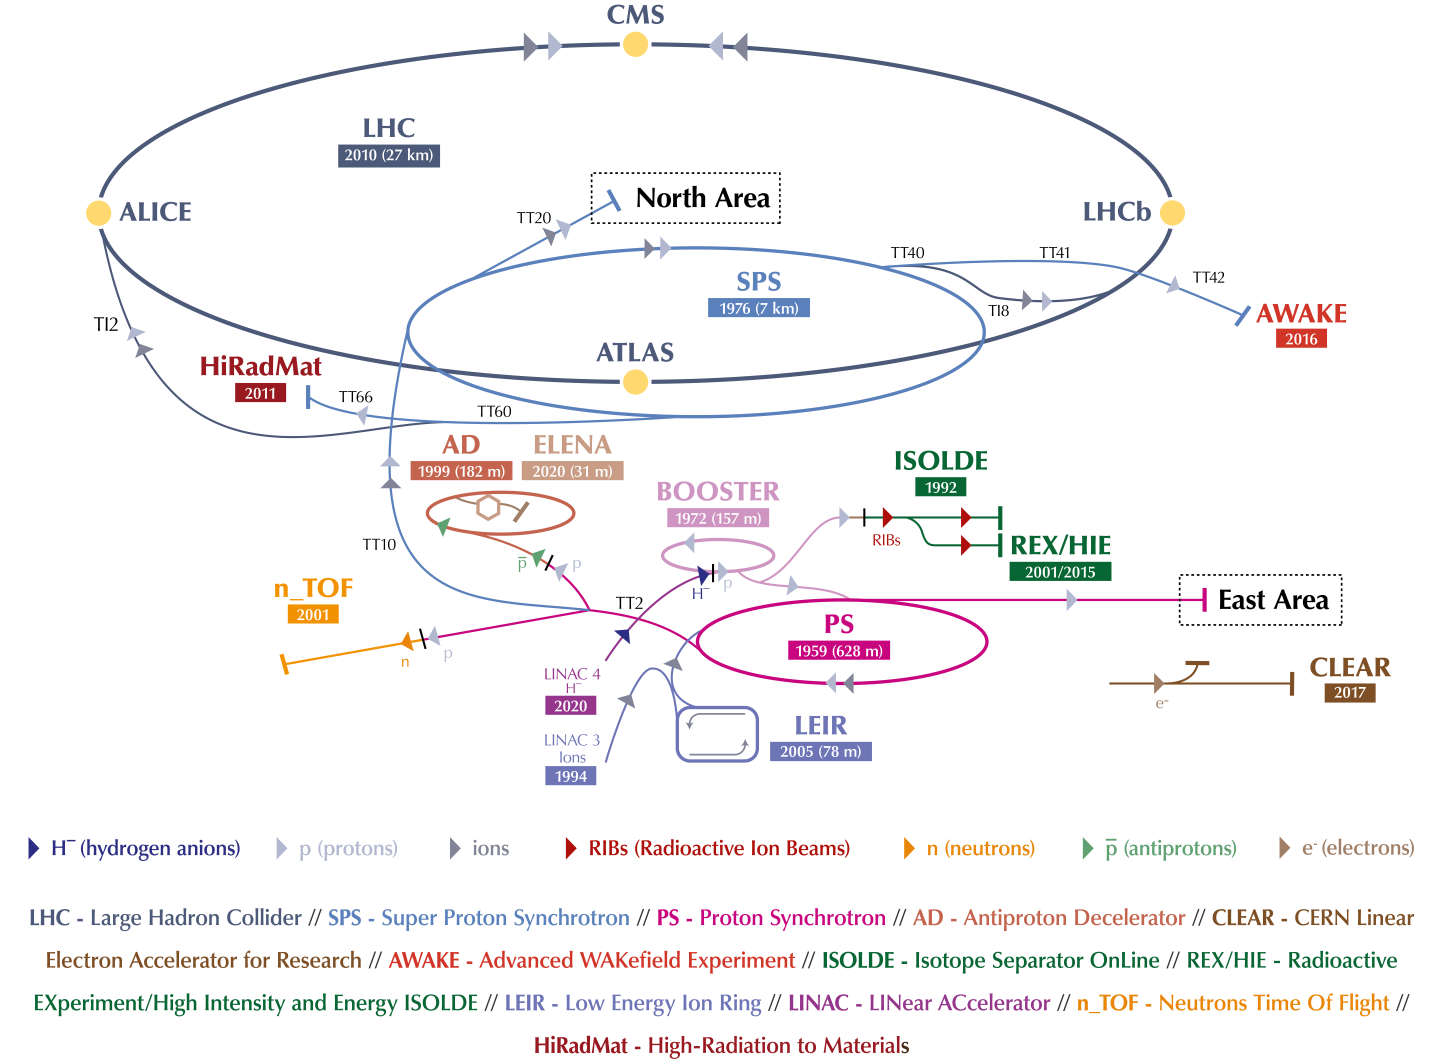
\includegraphics[width=0.9\columnwidth]{Figure_AcceleratorChain/cernComplex.png}
    \caption{CERN Accelerator Complex \parencite*[][]{ref:cerncomplex} . }
    \label{fig:AccComplex}
\end{figure}

CERN has not only provided advancements in fundamental sciences but has also pushed the frontiers of technology, with inventions such as the world wide web (www), Positron Emission Tomography (PET), etc. which have a positive impact on society globally.

CERN's accelerator complex (See \ref{fig:AccComplex} ) consists of many different types of linear and circular accelerators and interconnecting transfer lines to gradually accelerate the particles before injection into the Large Hadron Collider (LHC). 

Since 2020, Linear accelerator 4 (Linac4) became the source of proton beams for the LHC. Linac4 is an 86 \si{\meter} long machine. It accelerates negative hydrogen ions up to 160 \si{\mega \electronvolt}. The ions are then stripped of their two electrons during injection from Linac4 into the Proton Synchrotron Booster (PS Booster or PSB) to leave only protons. The PS Booster is made up of four superimposed synchrotron rings, with a 157 \si{\meter} circumference, which accelerates the injected protons up to 2 GeV for injection into the Proton Synchrotron (PS). 

Currently, the PS is the oldest accelerator in the chain. With a circumference of 628 meters, the PS operates up to 26 \si{\giga \electronvolt}. The Super Proton Synchrotron (SPS) is the second largest machine in the complex, measuring nearly 7 \si{\kilo \meter} in circumference. It takes the particles from the Proton Synchrotron and accelerates them up to 450 \si{\giga \electronvolt}. The CERN accelerator complex culminates with the Large Hadron Collider. The LHC consists of a 27 \si{\kilo \meter} ring of superconducting magnets, which guide two high-energy particle beams traveling in the opposite directions in separate beam pipes. The beams collide at four locations around the accelerator ring, corresponding to the positions of four particle detectors ATLAS, CMS, ALICE and LHCb. The High Luminosity Large Hadron Collider ( HiLumi LHC) project aims to deliver proton-proton collisions at 14 \si{\tera \electronvolt}.

\begin{figure}[h]
    \centering
    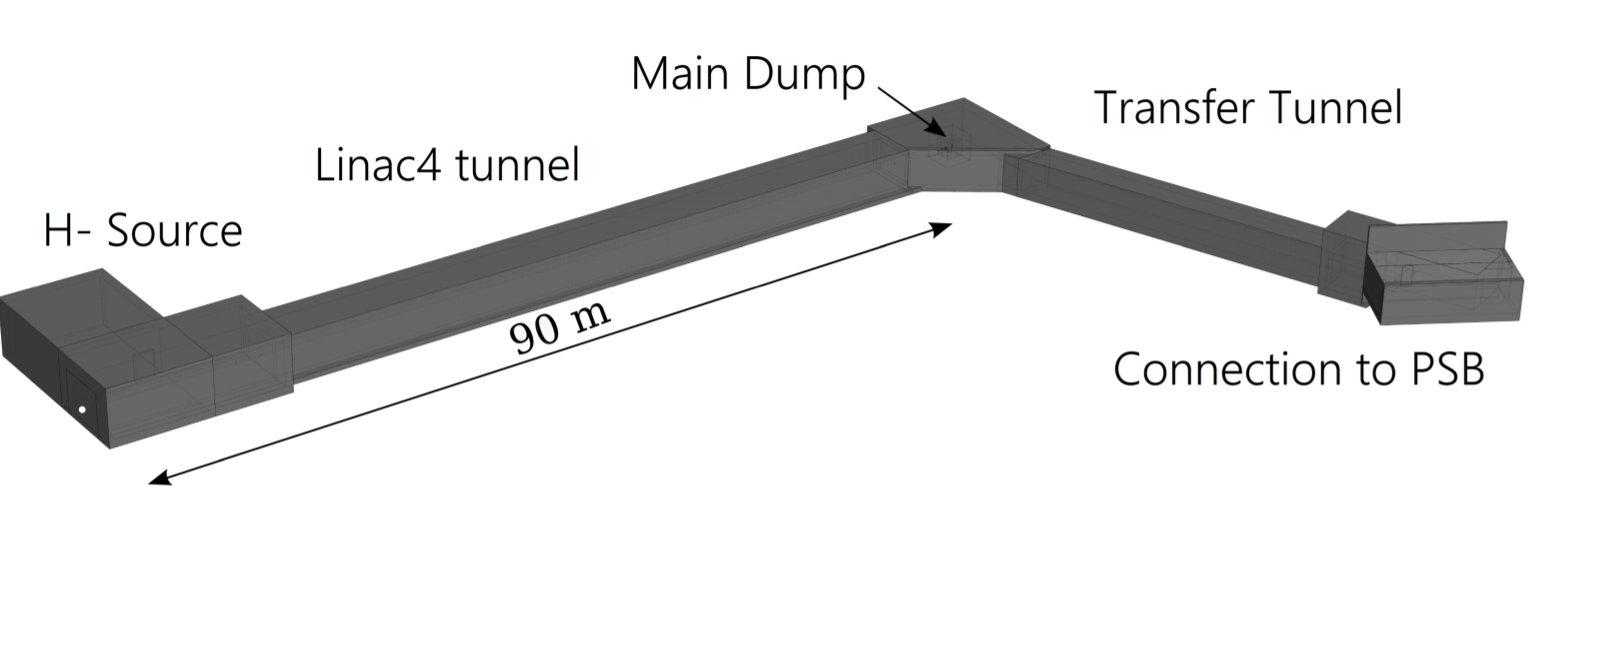
\includegraphics[width=0.70\columnwidth]{Linac4_Layout/linac4_Layout.png}
    \caption{General Layout of LINAC4 and its transfer-line to the PSB. }
    \label{fig:Linac4_layout}
\end{figure}

Not only protons can be accelerated at the CERN accelerator complex. Linear accelerator 3 (Linac 3) is the starting point for the ions. It provides mainly lead ions, but also argon and xenon were used in the past. Experiments with oxygen are planned for the future. The long pulses of lead ions from Linac 3 are transformed into short, dense bunches by the Low Energy Ion Ring (LEIR) before they are injected into the PS. 

The injector chain apart from feeding the LHC is also used to deliver particles to several other experiments carried out at CERN, including Antimatter research on the Antiproton Decelerator (AD) and Extra Low ENergy Antiproton (ELENA), radioactive ion beam research on ISOLDE, research on neutron-nucleus interactions on the n-TOF facility, research on radiation-induced damage on materials in the HiRadMat facility and even studies on the use of proton-driven plasma wake-fields in AWAKE. 

\section{Linear Accelerator 4 (LINAC4)}
\label{sec:LINAC4}

As part of the LHC injection upgrade (LIU), CERN approved in 2007 the construction of LINAC4, to substitute the, by then existent, LINAC2 accelerator. The main goal for the construction of LINAC4 was to increase the beam brightness out of the PSB by a factor of 2, making possible an upgrade for the LHC injectors for higher intensity and eventually an increase of LHC luminosity \parencite*[]{ref:LIU}. 

The increase in beam brightness is achieved by combining two effects, the increase of the top energy to \SIlist[]{60}{\mega \electronvolt} (compared to the \SI[]{50}{\mega \electronvolt} given by LINAC2), which reduces significantly the space charge effect causing emittance blow up in the PSB. Secondly, the use of $H^{-}$ ions instead of protons makes it possible to inject into the PSB via the charge exchange scheme, which is explained in detail in Chapter \ref{ch:H0Hm}.

\begin{figure}[h]
    \centering
    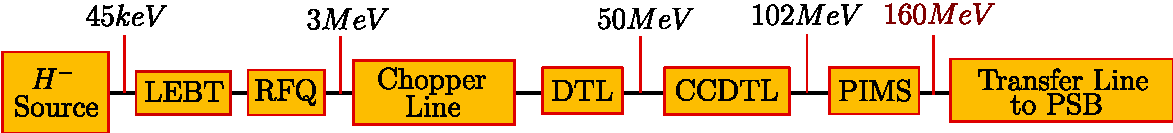
\includegraphics[width=1.0\columnwidth]{Linac4_AcceleratingPart/Linac4_acc.pdf}
    \caption{LINAC4 accelerating components layout. }
    \label{fig:Linac4_acc}
\end{figure}

LINAC4 is \SI[]{86}{\metre} long and is located 12 m below ground. Figure \ref{fig:Linac4_layout} shows the source, tunnel, dump and transfer line to the PSB. Beams began to be produced in 2013 and the milestone energy of \SIlist[]{160}{\mega \electronvolt} was reached in 2016, after the commissioning of all the accelerating structures. During the long shut-down (2019-2020), LINAC4 finally replaced LINAC2 as the source of protons for the LHC. 

A more detailed description of the architecture of the accelerating section of LINAC4 is shown in figure \ref{fig:Linac4_acc}. The accelerating sequence is quite standard for a pulsed LINAC design. The LINAC4 source is a cesiated molybdenum-surface radio-frequency plasma ion source \parencite*[][]{ref:SourceCite}. This source can produce $H^{-}$ ion beams of up to 400\si[]{\micro \second} pulse length, 40\si[]{\milli \ampere} at a maximum revolution frequency of \SI[]{0.8}{\hertz}

The Low Energy Beam Transport (LEBT) line provides the beam matching from the source to the RFQ (Radio Frequency Quadrupoles) and contains the diagnostics to monitor the source. The three meter RFQ performs the beam capture and bunching and accelerates the particles to an energy of 3\si[]{\mega \electronvolt}. It is followed by a Medium Energy Beam Transport (MEBT) or "Chopper Line". This system consists of an electrostatic beam deflector followed by a beam dump. The purpose of this line is to avoid losses at higher energies when the induced radiation is higher.

\begin{figure}[h]
    \centering
    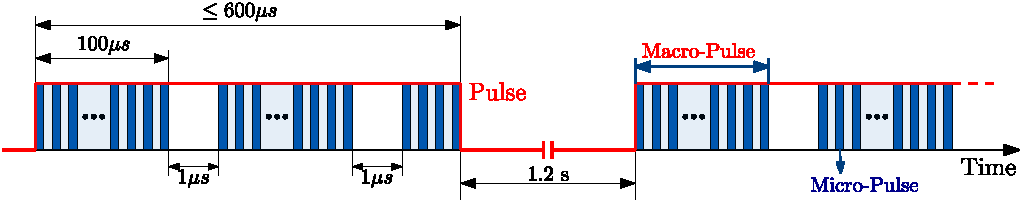
\includegraphics[width=1.0\columnwidth]{Figure_Linac4PulseStructure/Linac4_PulseStruct.pdf}
    \caption{LINAC4 Pulse Structure }
    \label{fig:Linac4PulseStruct}
\end{figure}


Three types of losses are treated with this system. Firstly, losses due to instable LINAC4 pulses. Secondly, it can be used to clean the first few tens of \si[]{\micro \second} of the beam pulse which are generally not stable. Finally, its purpose is to create "holes" in the beam pulse, timed with the rise-time of the PSB distributor, which switches the incoming LINAC4 beam between the four Booster Rings.  

The chopping line is followed by a series of three accelerating structures. The Drift Tube Linac (DTL) is divided in three tanks and accelerates the beam up to 50\si[]{\mega \electronvolt}. The Cell-Coupled Drift Tube Linac (CCDTL) is made of 7 accelerating modules for a top energy of 102 \si[]{\mega \electronvolt}. Finally, the Pi-Mode Structure (PIMS) brings the energy of the beam to the desired 160 \si[]{\mega\electronvolt}. More information about LINAC4 and its conforming parts can be found in \parencite*[]{ref:Linac4Technical}.  

In the current operational conditions, the LINAC4 pulse structure consists of four individual macro pulses, typically 20 - 100  \si[]{\micro \second}long (depending on the required number of injected turns per ring) and separated by a 1 \si[]{\micro \second} particle-free gap (See figure \ref{fig:Linac4PulseStruct}). Each macro-pulse consists of a train of 500 \si[]{\pico \second} long micro-bunches that are spaced by intervals of 2.8 \si[]{\nano \second} \parencite*[]{ref:Linac4PulseStruct}. In this document, we will focus on the beam pulse, that is, the convination of this four macro pulses.


\section{Proton Synchrotron Booster (PS Booster)}

The PS Booster or PSB has a circumference of 157 m and the unique characteristic of having 4 superimposed rings. Each of the rings hosts one bunch per cycle, and this allows to have 4 times the intensity delivered to the PS for each pulse of the Linac. Every ring has 16 equal periods (i.e. sequence of components) of 9.8 m each (See figure \ref{fig:PSB}).  The cycle length is 1.2 s. 

After the LIU upgrade the injection energy was upgraded from 50 MeV (from Linac2) to 160 MeV (from Linac4). The booster injection (BI) line and the injection region were fully upgraded during LIU. The changes in the injection will be explained in detail in chapter \ref{ch:H0Hm}. The beam is extracted from the booster at 1.4 GeV, however an energy upgrade up to 2 GeV is already planned. 

\begin{figure}[h]
    \centering
    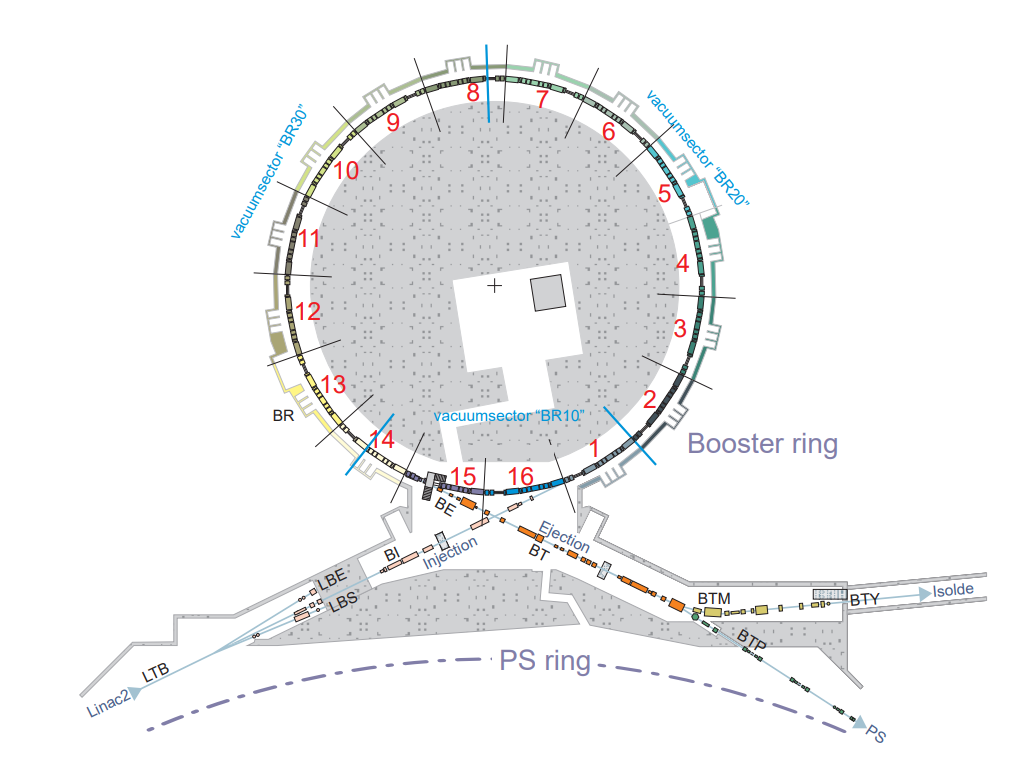
\includegraphics[width=0.8\columnwidth]{Figure_BoosterRing/BoosterRing.png}
    \caption{PSB Ring Schematic Layout.}
    \label{fig:PSB}
\end{figure}



\section{Accelerator Physics Principles}
\label{sec:AccPhysPrinc}

The topic of Accelerator physics is very broad, in this section only an overview of the topics of interest for this document will be introduced. These topics include a quick overview of the basic concepts of beam dynamics, transverse plane, beam size and emittance. For a much more complete introduction to the world of accelerator check \parencite*[][]{ref:BookAccPhysics}.

\subsection{Principles of beam dynamics}
\label{subsec:PrincBeamDyn}

For describing the movement of the particles in an accelerator, the Frenet-Serret coordinate system, shown in figure \ref{fig:CoordinateSystem}, is commonly used. S defines the longitudinal coordinate and it is always tangent to the reference path. X and Y define the transverse plane (orthogonal to the particle trajectory). x(s) and y(s) describe the particle's deviation from the reference path at each point. $\rho(s)$ commonly defines the curvature of the reference orbit at each point. 


\begin{figure}[h]
    \centering
    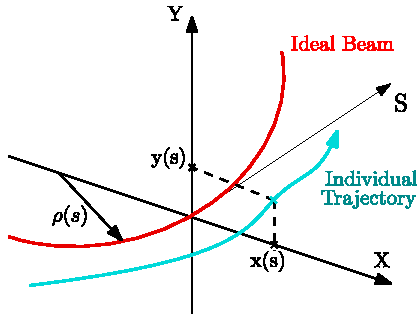
\includegraphics[width=0.5\columnwidth]{Figure_CoordinateSystem/CoordinateSystem.pdf}
    \caption{Frenet-Serret coordinate system.}
    \label{fig:CoordinateSystem}
\end{figure}

The theoretical conception of an accelerator starts by assuming constant energy and a stable beam trajectory. The scope of a particle accelerator design is to guide the beam of particles along the reference path and accelerate them to the desired energy. This is achieved by applying electromagnetic forces to the charged particles. Lorentz's law describes the force acting on a particle of charge "q" traveling in an electromagnetic field:

\begin{equation}
    \vec{F} = q \left( \vec{E} + \vec{v} \times  \vec{B}\right)
    \label{eq:LorentzLaw}
\end{equation}

Where $\vec{E}$ and $\vec{B}$ are the electric and magnetic fields and $\vec{v}$ is the particle velocity. Longitudinal electric fields accelerate the particles, while the transverse bending and focusing are provided by transverse magnetic fields. 

Particles which at the time $t_0$ have a non zero transverse coordinate $\left(x_0 , y_0 \right)$ and momentum $\left(x_{0}^{'} , y_{0}^{'} \right)$ start to perform oscillations in the horizontal and vertical planes,  called Betatron oscillations \parencite*[][]{ref:BookAccPhysics2}. These oscillations depend on the magnetic fields in the ring. The equation of motion on the transverse space can be derived from Lorentz's equation, and after some approximations it reads \parencite*[][]{ref:ApproxEqMotion}:

\begin{equation}
    \begin{aligned}
        x^{''} + \left(\frac{1}{\rho^{2}(s)}+\frac{1}{B\rho}\frac{\partial B_y(s)}{\partial x} \right)  x = 0 \\
        y^{''} - \frac{1}{B \rho}\frac{\partial B_y (s)}{\partial x}  y = 0
    \end{aligned}
    \label{eq:EqMotion}
\end{equation}


The product $B \rho$ is the magnetic rigidity and is equal to the ratio of the momentum to charge $p/q$. The only difference between the vertical and horizontal coordinates is the term $1/\rho^2(s)$ which is related to the centripetal force in the radial direction. These types of differential equations are often referred to as Hills equation \parencite*[][]{ref:HillEquation}, and describe a pseudo harmonic oscillator in which the spring constant depends on the position (s). For each element on the beamline, one can calculate the solution of the equation of motion. The solution of the equation can be expressed in a matrix formulation \parencite*[][]{ref:MatrixForm}:

\begin{equation}
    \begin{bmatrix}
        u(s) \\ u^{'}(s) 
   \end{bmatrix}
   = 
   \begin{bmatrix}
        C(s) & S(s) \\ C^{'}(s)  & S^{'}(s)
   \end{bmatrix}
   \begin{bmatrix}
        u_0 \\ u^{'}_0
   \end{bmatrix}
   =
   M(s) 
   \begin{bmatrix}
        u_0 \\ u^{'}_0
   \end{bmatrix}
\end{equation}

Where $M(s)$ is called the transformation matrix, which can be calculated individually for each type of beamline element. This matrix formalism is very useful as one can follow a particle trajectory along a complicated beam line by repeated matrix multiplication from element to element \parencite*[][]{ref:MatrixTransport}. Three commonly used transport matrices would be the following: 

\begin{itemize}
    \item Drift (no magnetic elements) of length L:
    
    \begin{equation}
        M_D
        =
        \begin{pmatrix}
             1 & L \\ 0 & 1
        \end{pmatrix}
    \end{equation}

    \item Focusing Quadrupole: 
    
    \begin{equation}
        M_{QF} =
        \begin{bmatrix}
             cos\left(\sqrt{k}L_Q\right) & \frac{1}{\sqrt{k}}sin\left(\sqrt{k}L_Q\right) \\
             -\sqrt{k}sin\left(\sqrt{k}L_Q\right) & cos\left(\sqrt{k}L_Q\right)
        \end{bmatrix}
    \end{equation}

    \item Defocusing Quadrupole:
    
    \begin{equation}
        M_{QD} =
        \begin{bmatrix}
             cosh\left(\sqrt{\left|k\right|}L_Q\right) & \frac{1}{\sqrt{\left|k\right|}}sinh\left(\sqrt{\left|k\right|}L_Q\right) \\
             -\sqrt{\left|k\right|}sinh\left(\sqrt{k}L_Q\right) & cosh\left(\sqrt{\left|k\right|}L_Q\right)
        \end{bmatrix}
    \end{equation}

\end{itemize}

In these equations, $L_Q$ refers to the length of the magnets and k is the effective focusing strength of the quadrupoles. 


\subsection{Particle beams and beam profile}
\label{subsec:TransBeamProf}

A beam or a bunch of particles is a collection of a very large number of particles whose center of gravity moves in a well-defined direction. If we consider the transverse plane X-Y (orthogonal to the beam direction of motion), one can obtain the particle distribution by noting the position of each particle that crosses this plane. If there is no coupling between the motion of the particles in the x and y directions, the distribution of the particles will be somehow elliptical, with the axis of the ellipse parallel to the x and y axes. See Figure \ref{fig:TransversePlane} for an example of transverse space particle distribution. 

\begin{figure}[h]
    \centering
    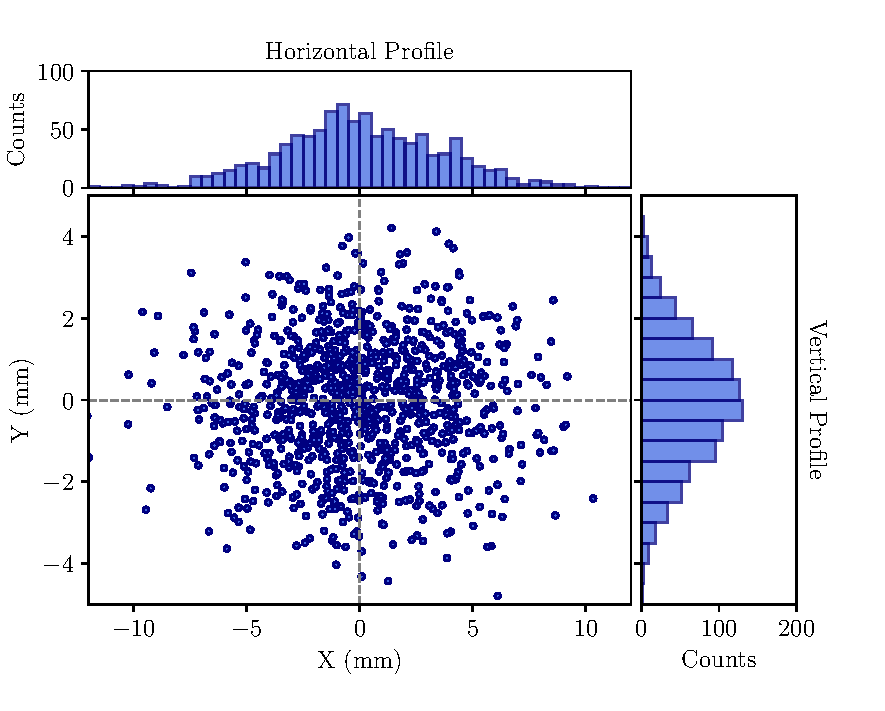
\includegraphics[width=0.9\columnwidth]{Figure_ParticlePositionExample/ParticlePosition.pdf}
    \caption{Example of Particle distribution in the X-Y space, with their corresponding projections.}
    \label{fig:TransversePlane}
\end{figure}

A histogram expressing the number of particles in a beam as a function of the transverse position is known as a beam profile. A Horizontal beam profile gives information about the number of particles at different x positions. A Vertical beam profile gives information about the number of particles at different y positions. 

A typical way of expressing the number of particles at a certain point in space is using a gaussian function:

\begin{equation}
    N(x,y) = \frac{N_{Tot}}{2\pi\sigma_x \sigma_y}\cdot exp\left(-\frac{1}{2}\left(\left(\frac{x-x_0}{\sigma_x}\right)^2 -\left(\frac{y-y_0}{\sigma_y}\right)^2\right)\right)
    \label{eq:GaussianDist}
\end{equation}

Here $x_0 , y_0$ are the coordinates of the center of the beam. $\sigma_x , \sigma_y$ are the standard deviation of the normally distributed beam of particles. $N_{Tot}$ refers to the total number of particles in the beam pulse. However, this expression is no more than an approximation, and one should be careful to understand its limitations. Usually, at the particle source, the beam of particles is far from Gaussian, but after some acceleration, this becomes a good approximation \parencite*[][]{ref:BookAccPhysics}.

\subsection{Transverse phase space}
\label{subsec:TransPhSp}

Each one of the particles in the beam will not only have a different position, but also a different direction of movement. The velocity vector of each particle can be decomposed into two components, one parallel to the beam direction (s) and one orthogonal to it (transverse velocity). The transverse velocity can then be discomposed into its components along the x-axis and y-axis. The phase space has information on both the position and the transverse velocity of each of the particles in the beam. Because the velocity and the momentum of the particles are related, one can express the information of the phase space in terms of the transverse momenta of the particles $\left(p_x , p_y \right)$. 

For convenience, the phase space is described by the transverse momentum $(p_x , p_y)$ normalized by the longitudinal momentum $(p_s)$. This quantities are expressed by: $x^{'} = p_x / p_s$ and $y^{'} = p_y / p_s$. For reprsenting the phase space, two charts are needed, one for the vertical plane and one for the horizontal plane. Figure \ref{fig:PhaseSpace} shows an example of particle distribution in the phase space. 

\begin{figure}[h]
    \centering
    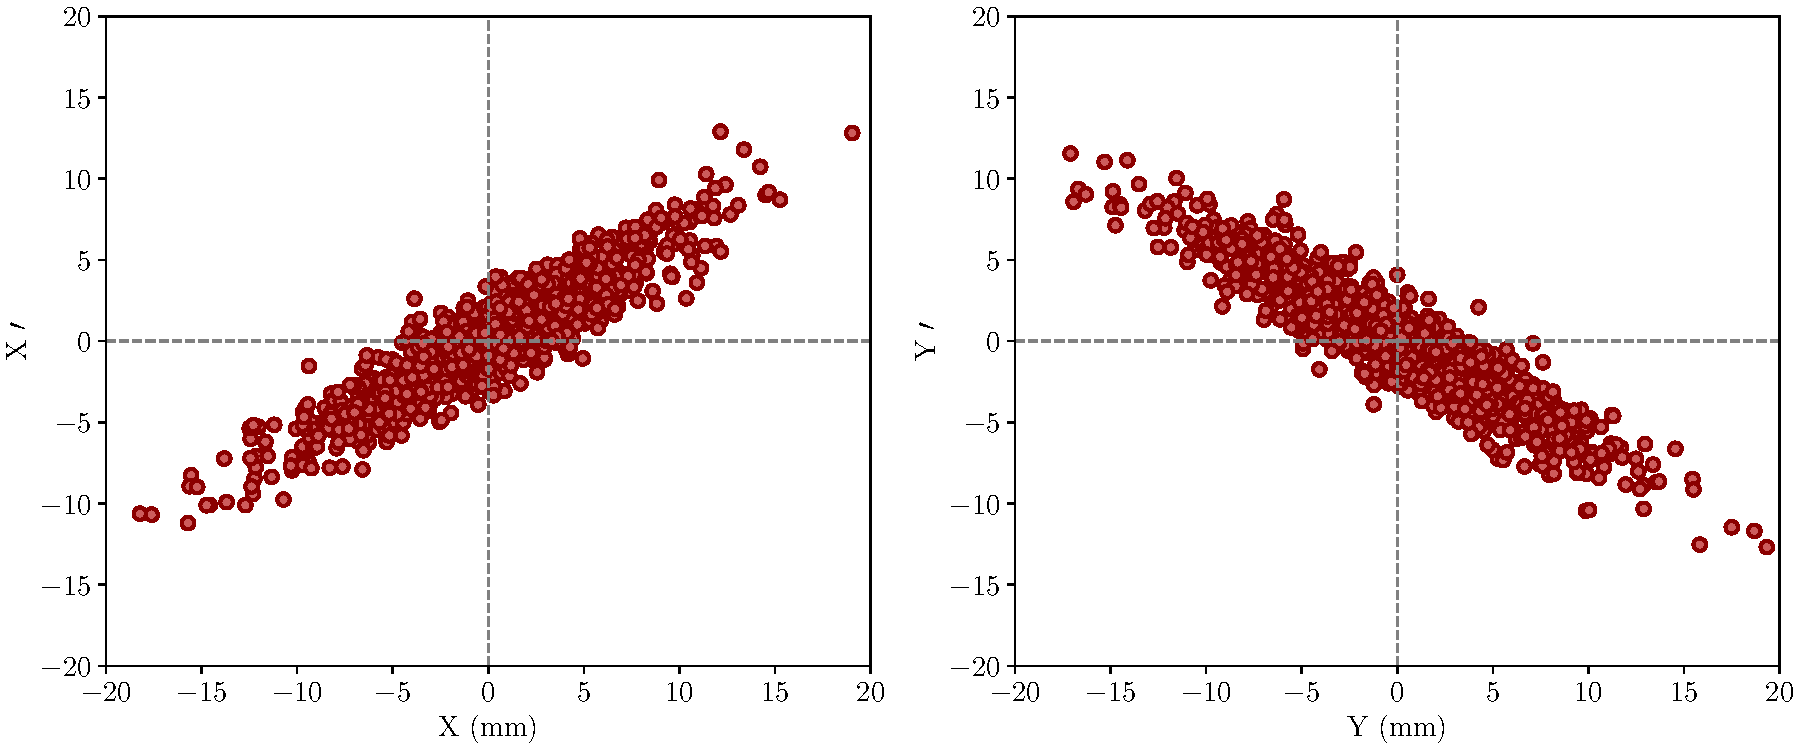
\includegraphics[width=1.0\columnwidth]{Figure_PhaseSpaceDist/PhaseSpaceDist.pdf}
    \caption{Particle distribution in the transverse phase space. }
    \label{fig:PhaseSpace}
\end{figure}

The particle distributions in the phase space are again ellipses, but in this case, they are tilted with respect to the axes. The phase space contains the whole description of the states of all the particles for a particular plane. This information is needed if one wants to calculate the subsequent motion of the particles in the electromagnetic fields of the accelerator. 

\subsection{Transverse beam emittance}
\label{subsec:TransBeamEm}

A formal description of the phase space can be developed by exploiting the elliptical shape of the phase space. The equation of the phase-space ellipse can be described as follows: 

\begin{equation}
    \epsilon = \gamma x^2 + 2\alpha x x^{'} + \beta x^{'2}
    \label{eq:ellipse}
\end{equation}

The parameters $\alpha, \beta, \gamma$ are referred to as the Courant-Synder parameters \parencite*[][]{ref:BookAccPhysics}. The area of the ellipse is simply $A = \pi \epsilon$. In the accelerator and beam physics language, the area in the phase space ($\epsilon$) containing the particles is called the emittance, statistical emittance, or more precisely it is called the rms-emittance. In the case of Gaussian beams, the concept of rms-emittance can be directly interpreted as the area containing a fraction (f) of ions. For example, it can be proven \parencite*[][]{ref:BookAccPhysics2},  that the curve of area $\epsilon$ should contain a $39\%$ of particles. Table \ref{tab:ParticleProportion} resumes the fraction of particles in a gaussian beam associated with various emittances. 


\begin{table}[h]
    \centering
    \begin{tabular}{cc}
    \hline
    Emittance $\epsilon(f)$ & Particle Fraction ($\%$) \\ \hline
    $\epsilon_{rms}$       & 15                     \\
    $\pi \cdot \epsilon_{rms}$     & 39                     \\
    $2\pi \cdot \epsilon_{rms}$  & 63                     \\
    $4\pi \cdot \epsilon_{rms}$  & 86                     \\
    $8\pi \cdot \epsilon_{rms}$   & 98                     \\ \hline
    \end{tabular}
    \caption{Fraction (f) of particles in a Gaussian beam associated with different definitions of emittance.}
    \label{tab:ParticleProportion}
\end{table}

\begin{figure}[h]
    \centering
    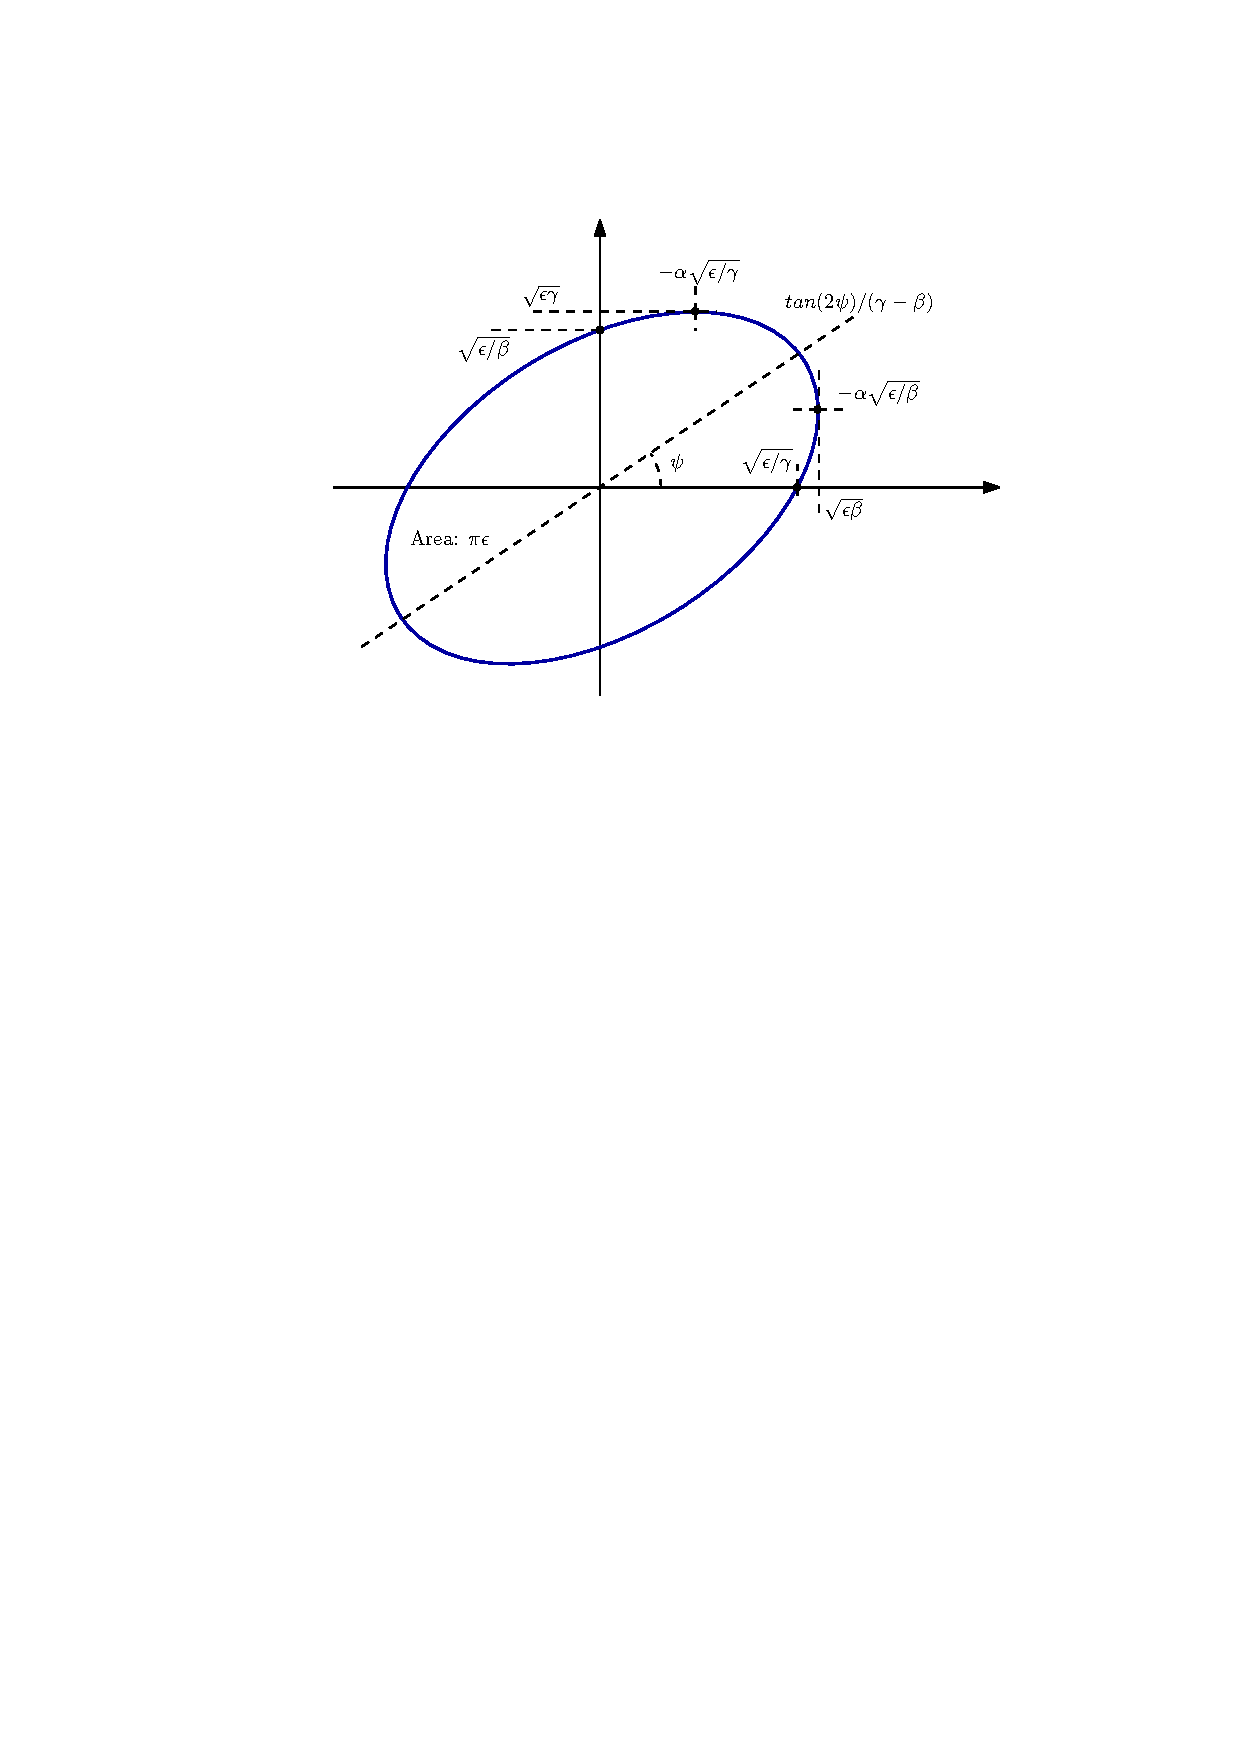
\includegraphics[width=0.7\columnwidth]{Figure_GeometricEmittance/GeometricEmittancve.pdf}
    \caption{Phase Space, geometrical ellipse. }
    \label{fig:CouranSnyder}
\end{figure}

    
Figure \ref{fig:CouranSnyder} shows a geometrical description of the Courant-Snyder parameters. These parameters $\left(\alpha , \beta , \gamma \right)$ are not independent, the third parameter is typically defined in therms of the other two: 

\begin{equation}
    \gamma = \frac{1 + \alpha^{2}}{\beta}
\end{equation}

Some other quantites, also very important for the understanding of the mathematical formulation of the transverse emittance are the following: 

\begin{equation}
    x_{rms}^2 = \left<x^2\right> =\frac{1}{N}\sum_{i=1}^N x_i^2
\end{equation}
\begin{equation}
    x_{rms}^{'2} = \left<x^{'2}\right> = \frac{1}{N}\sum_{i=1}^N x_i^{'2}
\end{equation}
\begin{equation}
    x x^{'}_{rms} =  \left< x x^{'}\right> = \frac{1}{N}\sum_{i = 1}^{N} x_{i} x^{'}_{i}
\end{equation}

With $x_{i} = X_{i} - \left< X \right>$ and $x^{'}_{i} = X_{i} - \left< X^{'}\right>$. $X_{i}$ and $X_{i}^{'}$ being the horizontal position and momentum of the individual particles conforming the beam. For convenience this parameters can be expressed in a matrixs form as follows: 

\begin{equation}
    \Sigma = 
    \begin{pmatrix}
        \left< x^{2} \right> & \left< x x^{'} \right> \\
        \left< x x^{'} \right> & \left< x^{' 2} \right>
    \end{pmatrix}
    = \epsilon 
    \begin{pmatrix}
        \beta & - \alpha \\ -\alpha  & \gamma
    \end{pmatrix}
\end{equation}

The rms-emittance ($\epsilon$) can also be obtained from this parameters as follows: 

\begin{equation}
    \epsilon = \pi \sqrt{\left<x^{2}\right>\left< x^{'2}\right> - '\left<x x^{'}\right>^{2}}
\end{equation}

\subsection{Phase Space Evolution}
\label{subsec:PhaseSpaceEvol}

In a transfer line or a storage ring (i.e. no acceleration), and assuming no energy losses due to radiation, Liouville's theorem establishes that emittance ( considering both transverse and longitudinal coordinates) is conserved \parencite*[][]{ref:EmittanceConserv}. However, the shape of the ellipse changes along the beam line. Figure \ref{fig:PhasSpaceEvol} illustrates a typical example of phase space evolution. 

\begin{figure}[h]
    \centering
    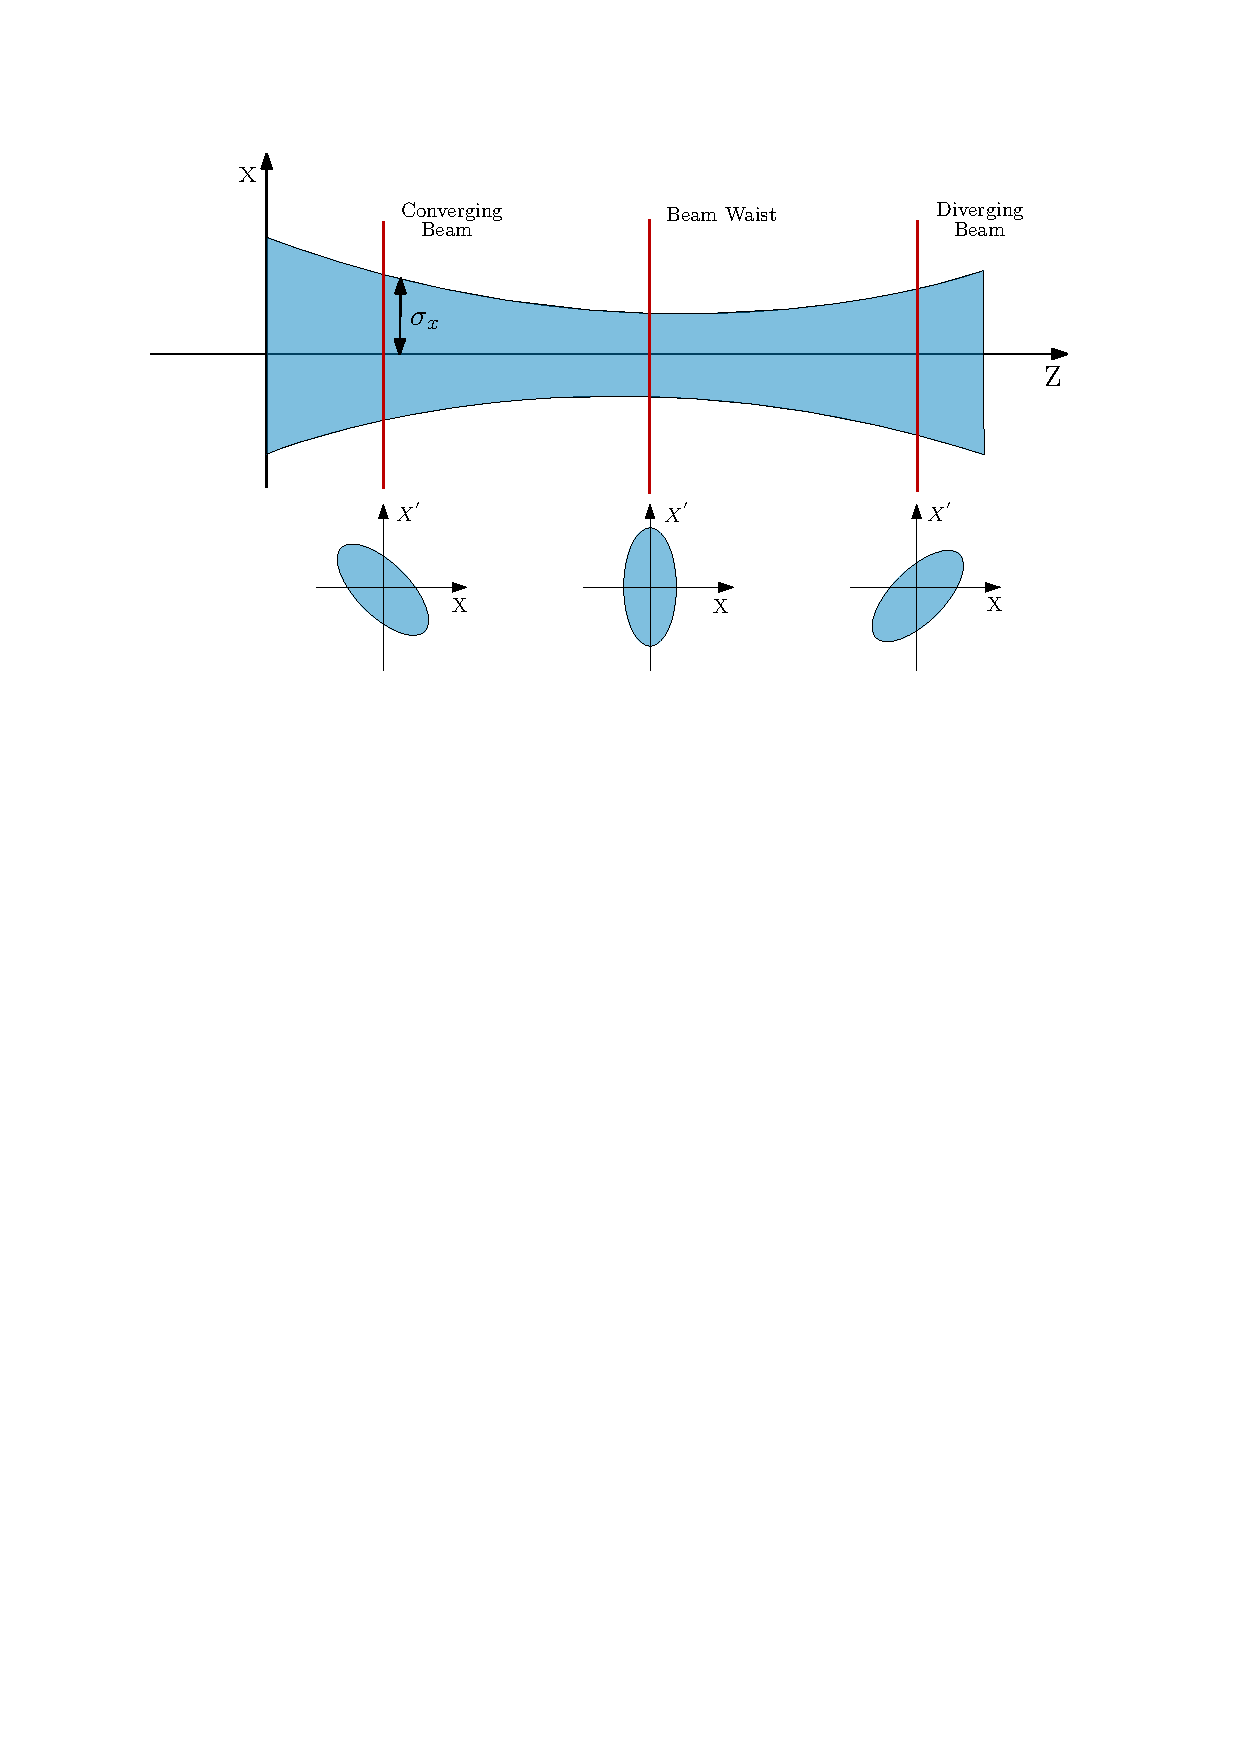
\includegraphics[width=0.9\columnwidth]{Figure_BeamEvolution/BeamEvolution.pdf}
    \caption{Example of phase space evolution. }
    \label{fig:PhasSpaceEvol}
\end{figure}

In the previous sections (Sec. \ref{subsec:PrincBeamDyn}) we saw how, in linear systems, points on the phase-space could be mapped from one location to the other through matrix multiplications. Similarly, assuming the following single-particle transport matrix:

\begin{equation}
    \begin{bmatrix}
         x_1 \\ x_1^{'} 
    \end{bmatrix}
    = 
    \begin{bmatrix}
       c & s \\ c^{'} & s^{'}
     \end{bmatrix}
     \begin{bmatrix}
        x_0 \\ x_0^{'}
     \end{bmatrix}
\end{equation}

After some algebraic calculations, one can obtain the following transport matrix for the Twiss parameters \parencite*[][]{ref:MatrixToTwiss}:

\begin{equation}
    \begin{bmatrix}
       \beta_1 \\ \alpha_1 \\ \gamma_1
    \end{bmatrix}
    =
\begin{bmatrix}
   c^2 & - c s & s^2 \\ -c c^{'} & cs^{'} + c^{'}s & -s s^{'} \\ c^{'2} & -2c^{'}s^{'} & s^{'2}
\end{bmatrix}
=
\begin{bmatrix}
   \beta_0 \\ \alpha_0 \\ \gamma_0
\end{bmatrix}
\label{eq:MatrixEq}
\end{equation}

\section{Beam Diagnostics}

Beam diagnostics and instrumentation are essential constituents of any particle accelerator. They allow us to monitor the behavior and properties of the particle beam. Without adequate diagnostics, one would be blindly operating an accelerator and it would be impossible to assess problems and improve performances. Different accelerator types require different diagnostics. Similarly, different beam properties require very different instrumentation systems and techniques.  \parencite*[][]{ref:BeamInstrumentationBook}, \parencite*[][]{ref:NotesBeamInst} and \parencite*[][]{ref:CASbeamInst}, are very recommendable references, where the topic of beam instrumentation is covered extensively but yet with a very accessible approach. 

This chapter will focus on describing the principles of some commonly used devices that will be of great relevance for understanding the concepts of this work. We shall focus on the measurements of two beam properties: 

\begin{itemize}
    \item Transverse Beam Profile Measurements: They allow the measurement of the transverse distribution of the particles throughout the accelerator. This measurement is important to control the beam width and position, as well as the transverse matching between different parts of the accelerator facility. In particular, we will focus on Secondary Emission Grids (SEM Grids) and Wire Scanners. 
    \item Beam Intensity Measurements: They allow to measure the total electrical current of the beam, which is one of the most important parameters for the operation of a particle accelerator. Current measurements allow, for example, to determine the transfer efficiencies in linacs and transfer lines. In this case, we will talk about Beam Current Transformers (BCT) and Faraday Cups (FC).
\end{itemize}


\section{Seconday Emission Grids (SEM Grids)}
\label{sec:SEMgrids}

Wire Grids or Secondary Electron EMission grids (SEM Grid) are devices composed of a large number of parallel fixed wires or strips. Figure \ref{fig:SEMgrid} shows an example of a SEM grid detector. They are interceptive devices, during the measurements, each one of the wires interacts directly with the beam of particles. During this process a current, proportional to the number of particles, is generated in each wire.  By measuring the current in all the wires a beam profile can be reconstructed. More detailed explanations about the current generation process and the profile reconstruction will be given in Chapters \ref{ch:BeamMatterInter} and \ref{ch:CurrentModeling}.

\begin{figure}[h]
    \centering
    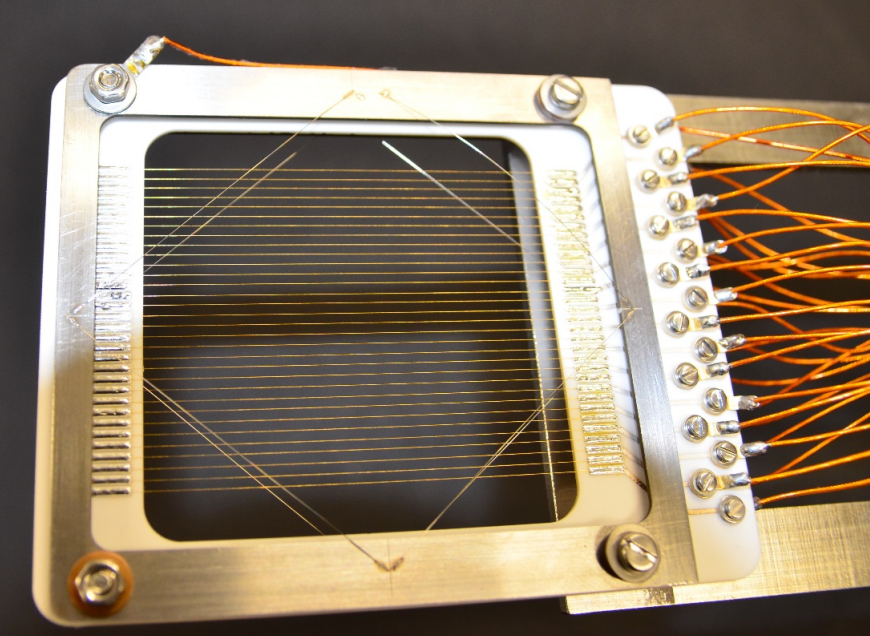
\includegraphics[width=0.6\columnwidth]{SEMGrid/semgrid.png}
    \caption{Example of a SEM grid installed at CERN accelerator Complex. }
    \label{fig:SEMgrid}
\end{figure}

SEM grids allow for a single-shot acquisition, and in some cases, it is possible to observe the evolution of the beam profile in the same pulse. The number of wires and the spacing between them varies from system to system. It is important for the detector to cover the whole range of the beam size and to have enough resolution to properly reconstruct the beam profile. Theoretically, a bigger detector with a larger number of wires would be more convenient. However, a system with too many wires implies an overly complicated acquisition system, it increases the probability of wire cross-talk and augments the construction costs. 

A typical number of wires ranges from 16 to 48. In some devices, the wires are spaced unevenly, with a denser distribution in the center. The diameter-to-spacing of the wires determines the attenuation of the beam current, which becomes an important parameter to consider for particles at low energies as they are fully stopped in the detector's material. It is common to consider that a $10 \%$ of the beam area is covered with the wires. 

The wire materials are selected to optimize signal generation and ensure proper thermal performance. Typical materials used for wire grid designs are Tungsten, Carbon (Graphite, CNT) or Titanium. The motion control of SEM grids is relatively simple, they are either fully inserted or fully retracted, and sometimes they might even be permanently positioned in the beam pipe with no motion control at all. 


\begin{figure}[h]
    \centering
    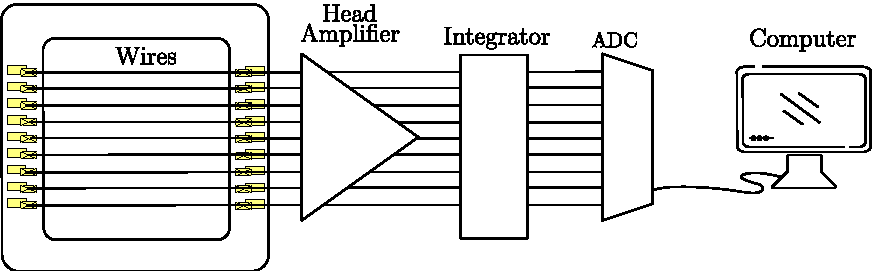
\includegraphics[width=1.0\columnwidth]{SEMgridDataADq/SEMdataAdc.pdf}
    \caption{Schematic representation of SEM Grid Adquisition system. }
    \label{fig:SEMGridReadOutSystem}
\end{figure}

Typically, the data acquisition chain is composed of a head amplifier that sits as near as possible to the grid, often in an area with radiation. It is followed by an integrator or signal conditioning circuit that sits away in a safe room. From the integrator, the signal is fed to a computer controller ADC. This scheme requires one signal cable per wire over the distance from the device to the ADC. 

The main drawbacks of this diagnostics device are the limit on the spatial resolution (which can be hardly reduced to less than a few hundred micrometers), the small wire signals and the complicated data adquisition system. 

\section{Wire Scanners}
\label{sec:WireScan}

Instead of using several wires with individual, expensive electronics, the Wire Scanners consist of a single wire that can be swept through the beam pipe (See figure \ref{fig:WireScan}). The main advantage of this technique is the high resolution that can be accomplished (sub-mm range). It is often used in accelerators with small beam sizes. These devices also intercept the beam of particles, however, its effect is practically negligible.

\begin{figure}[h]
    \centering
    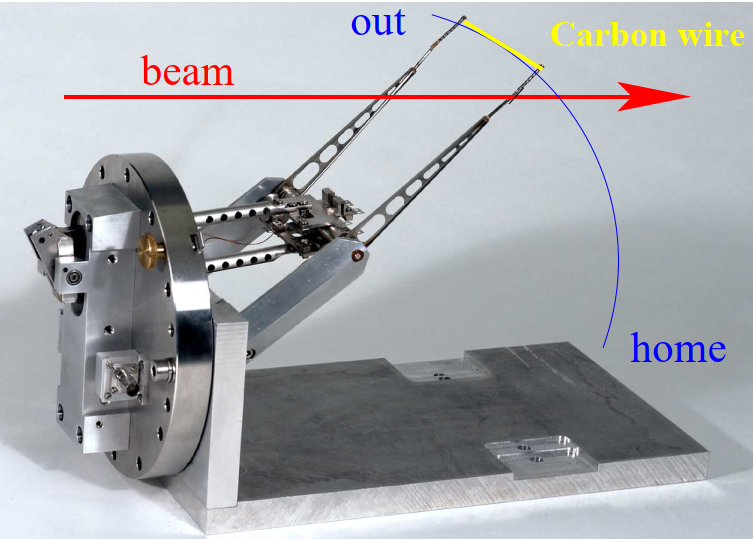
\includegraphics[width=0.6\columnwidth]{WireScanner/WireScanner.png}
    \caption{Rotational Fast Wire Scanner, used at CERN SPS. }
    \label{fig:WireScan}
\end{figure}

In the context of this thesis, we differentiate between two types of wire scanners:

\begin{enumerate}
    \item Slow Wire Scanners: They are commonly used on LINACs or transfer lines. Where the beam energy of the particle beam is small and the pulse structure consists of short pulses and low repetition rates. In this case, the profile is reconstructed by using the current generated in the detector by its interaction with the beam of particles. This signal is typically small and requires careful care in the acquisition. Usually, due to the low repetition rate of the beam in those areas, one sample is taken on each beam pulse, leaving plenty of time to move the wire from one pulse to the rest. 
    \item Fast Wire Scanners: For high energy and high repetition range beams, the profile is reconstructed by measuring a shower of secondary particles generated during the beam/wire interaction. These secondary particles might be hadrons (for proton/heavy ion accelerators) or photons (for electrons accelerators).  The secondary shower is detected outside the beam pipe, with a photo-multiplier tube. The speed of the wire movement varies over a very large range that can go from 1 \si[]{\metre /\second} up to 20 \si[]{\meter /\second}. In this case, the signal measured is typically quite large, due to the high photomultiplier range.  
\end{enumerate}

In both cases, the measurement of the wire position is a crucial aspect of the measurement, as the beam profile is reconstructed by correlating the wire position with the generated signal. The precision of the measurements of the wire scanner positions will therefore be a crucial factor in the measurement precision and resolution. In the case of fast wire scanners, the deformations or vibrations in the wire can also restrict the spatial resolution. Beam position and beam size variations during the measurement period can induce additional errors. 

For both, slow and fast wire scanners, the dimensions of the wire have a direct impact on the signal strengths and the measurement accuracy. In general beam sizes between 10 \si[]{\micro \metre} to 50 \si[]{\micro \metre}  are used.

\section{Beam Current Transformer (BCT)}
\label{sec:BCT}

An electric current flowing through a conductor gives rise to a magnetic field around the conductor, and passing a conducting loop through a magnetic field induces a current through the loop. These well-known principles of induction are used in the Beam Current Transformer (BCT). In this case, the particle beam is the primary current and can be described as: 

\begin{equation}
    I_{beam} = \frac{q e N_{part}}{t}
\end{equation}

Where $N_{part}$ is the number of particles of charge $q$ per unit time $t$. $e$ is the electron charge. This beam current generates a magnetic field as it travels through the accelerator. This magnetic field can be measured by placing a torus with high permeability around the beam. Some windings are placed around the tourus and then connected to an electrical circuit for read-out. Figure \ref{fig:BCTschema} shows a schematic representation of a BCT design. Measuring small beam currents becomes very challenging with these devices.

\begin{figure}[h]
    \centering
    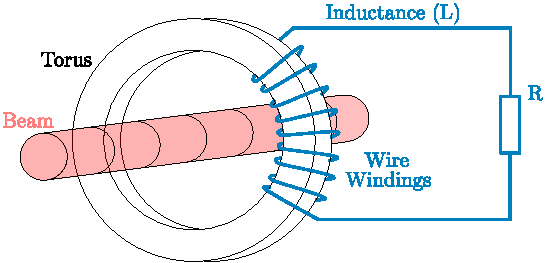
\includegraphics[width=0.6\columnwidth]{BCTschema/BCTschema.pdf}
    \caption{Schema of a current transformer built as a ring-core (torus). }
    \label{fig:BCTschema}
\end{figure}

\section{Faraday Cup (FC)}
\label{sec:FC}

A faraday cup (FC) is a beam stopper that measures the electrical current of the beam. A basic cup design is shown in figure \ref{fig:FaradayCup}. With a Faraday cup, a much lower current can be measured compared to a BCT, of the order of the \si[]{\pico \ampere} for low noise systems. These devices consist of an isolated metal cup connected to a current-sensitive pre amplifier. The current in these detectors is generated by measuring the total charge from the beam of particles that is deposited in them. High energetic particles not depositing all their energy in the detector material can affect negatively the measurement results. Similarly, a Secondary Electron (SE) suppression system has to be included in these devices to avoid errors in the current measurements. This is done by creating very long cups, high voltage suppression close to the entrance or by using a magnetic field. 

\begin{figure}[h]
    \centering
    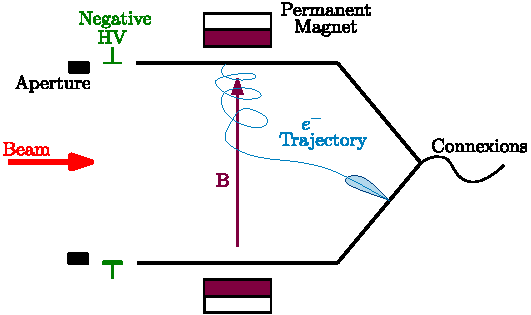
\includegraphics[width=0.6\columnwidth]{FCschema/FCschema.pdf}
    \caption{Schematic Representation of Faraday Cup. }
    \label{fig:FaradayCup}
\end{figure}

Sometimes, Faraday cups are also used for higher beam currents, where measurements with BCTs are also possible as they are easier to implement. In addition, cups serve as beam dumps. For high beam energies, one has to be concerned about the high thermal and structural shocks that these devices might suffer.



\chapter{Beam Matter Interaction} 
\label{ch:BeamMatterInter}
\pagestyle{fancy}

\graphicspath{ {Figures/Chapter2_BeamMatterInteraction/} }

While in-depth dissertations about the broad topic of particles interaction with matter can be found in literature~\parencite*[]{ref:Knoll,ref:Evans,ref:avernier}, 
this chapter will introduce the basics  necessary to introduce the subject and understand later chapters.

The interactions that we will focus on are primarily those related to Coulomb forces between the incident charged particle and the electrons and nuclei of the detector material. During these interactions, the incident charged particle loses its energy and can be deflected from its original path. In the case of heavy charged particles whose rest mass is large compared with that of the atomic electron, inelastic collisions with atomic electrons are usually the predominant interaction mechanism. In such encounters, the electrons in the medium might experience a transition to an excited state (excitation) or to an unbound state (ionization). 

\subsection{The Bethe Bloch Formula}
\label{sec:Bethe}

Stopping power is the parameter used to describe the gradual loss of energy of a charged particle as it penetrates into a medium. For a given incident heavy particle and target, this energy loss is highly dependent on the particle velocity. At moderately relativistic energy ranges ($10$ - $10^6$ \si[]{\mega \electronvolt}/amu), the electrostatic stopping power is well defined by the Bethe Bloch theory \parencite[]{ref:Bethe}. 

\begin{equation}
    - \left< \frac{dE}{dx} \right> = Kz^2_e\frac{Z}{A}\frac{1}{\beta^2}\left[ \frac{1}{2} ln \left( \frac{2m_e c^2 \beta^2 \gamma^2 T_{max}}{I^2}\right) -\beta^2 - \frac{\delta\left(\beta \gamma\right)}{2} \right]
    \label{eq:bethe}
\end{equation}

With the symbol and parameter definitions given in table \ref{tab:ParBethe}. The mean ionization energy is highly dependent on the material, and it can vary from a few \si[]{\electronvolt} for materials with low Z to a hundred of \si[]{\electronvolt} for materials with high Z. A good approximation can be formulated as follows \parencite*[][]{ref:IonizationEne}:

\begin{equation}
    I \left[ eV \right] = 10 \cdot Z 
    \label{eq:ionizationEnergy}
\end{equation}

The maximum energy that can be transferred to a target electron in a single head-on collision is described by $T_{max}$, and can be approximated by the following formula \parencite*[][]{ref:TmaxFormula}: 
\begin{equation}
    T_{max} = \frac{2m_e c^2 \beta^2 \gamma^2}{1+\frac{\gamma m_e c^2}{M c^2}+\left( \frac{m_e c^2}{M c^2} \right)^2}
    \label{eq:tmax}
\end{equation}

Finally, $\delta (\beta \gamma)$ is a parametrized density correction factor necessary for highly relativistic particles \parencite*[][]{ref:Bethe}, its units are $MeV cm^2 g^{-1}$. It is important to notice that the energy deposited will very much depend on the characteristics of the incident particle as well as the absorber $\left( -\left< \frac{dE}{dx} \right> \propto \frac{Z}{A}  \right)$. 

\begin{table}[h!]
    \centering
    \begin{tabular}{ccc}
    \hline
    \textbf{Symbol}                  & \textbf{Definition}                  & \textbf{Units or Value}                                               \\ \hline
    $N_A$                      & Avogadro's Number           & $6.0221415(10)\cdot10^23$ $mol^{-1}$ \\
    $z_e$                      & Charge of incident particle &                                                              \\
    Z                       & Atomic number of absorber   &                                                              \\
    A                       & Mass Number of absorber     &                                                              \\
    I                       & Mean excitation energy      & eV                                                           \\
    $\beta \gamma$              & Relativistic parameters     &                                                              \\
    $m_e c^2$ & Electron Mass $\cdot$ $c^2$          & 0.510998918(44) MeV                                          \\
    $r_e$                      & Clasical Electron Radius    & 2.8179403250(28) fm                                          \\
    M                       & Incident Particle Mass      & $MeV/c^2$\\
    
    K/A                     & $4 \pi N_A r_e^2 m_e c^2/A$ & 0.307075 $MeV g^{-1} cm^2$  \\
     $\alpha$ & fine-structure constant & 1/137 \\ 
     \hline
    \end{tabular}
    \caption{Summary of variables used in this section.}
    \label{tab:ParBethe}
\end{table}

 Figure \ref{fig:EneDep} shows as an example, a comparison between the energy deposition of protons for different materials, as a function of the incident particle energy.  In this particular case, when the material is assumed to be thin, the energy deposition increases until reaching a maximum, after which it starts decreasing. From the image, we can observe that the energy deposited in graphite and copper is larger, due to their smaller mass number. Tungsten, gold and lead present smaller energy deposition values, and are similar to one another, due to their close atomic mass number. 

 \begin{figure}[h]
    \centering
    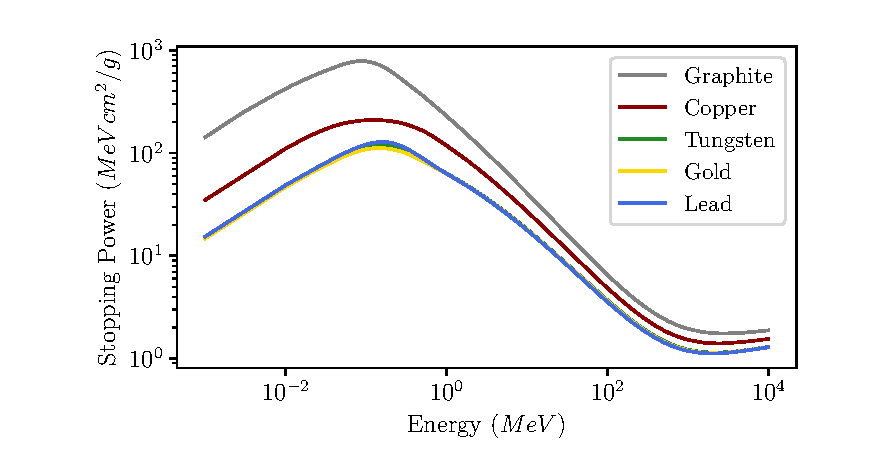
\includegraphics[width=1.0\columnwidth]{EdepMetal/EneDepMetal.pdf}
    \caption{Stopping power of protons in thin foils of different materials, as a function of incident particle energy. From \parencite*[][]{ref:NIST}.}
    \label{fig:EneDep}
\end{figure}

\subsection{Energy Loss in Mixtures and Compounds.}

One can consider a compound to be made up of very thin layers of pure elements in the right proportion. That is: 

 \begin{equation}
    \frac{dE}{dx} =  \sum w_j \left.\frac{dE}{dx} \right\vert_j
 \end{equation}

Where $\left. \frac{dE}{dx}\right\vert_j$  is the energy loss in the j-th component. However, it is important to remember that this is an approximation. The values of I and $\delta (\beta\gamma)$ are not perfectly represented by this addition method. More accurate values can be found in \parencite*[][]{ref:compound1} and \parencite*[][]{ref:compound2}, which include measured coefficients for nearly 200 mixtures and compounds. 

\subsection{Electrons Energy Loss}

For light particles such as electrons, bremsstrahlung losses are not negligible and can become dominant for energies above a few tens of \si[]{\mega\electronvolt}. One can define the critical energy $(E_c)$ as the point where the loss rates by Ionization and bremsstrahlung are the same \parencite*[][]{ref:EleCricEne}. 
\begin{equation}
    E_c = \frac{800}{Z + 1.2}
    \label{eq:ec}
\end{equation}

Figure \ref{fig:BremssVSion} shows the stopping power of electrons in a thin tungsten target, where we can observe the contribution of the radiative and collision interactions to the energy loss. In this case, radiative losses become relevant for incident electron energies $> 10 $\si[]{\mega\electronvolt}. This quantity is in agreement with equation \ref{eq:ec}.  

Some more information about how to model the energy losses due to this process can be found in \parencite*[][]{ref:BremstutorialG4}. However, in this thesis bremsstrahlung losses will be neglected, as we will always remain under the critical energy. 

\begin{figure}[h]
    \centering
    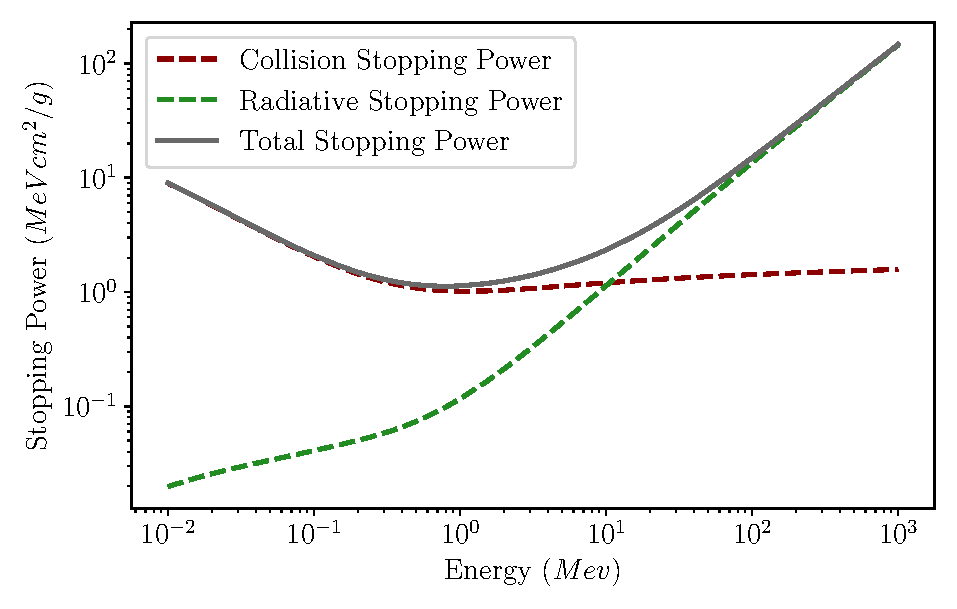
\includegraphics[width=1.0\columnwidth]{Electron_Edep/ElectronEdep.pdf}
    \caption{Stopping power of electrons in a thing tungsten foil, as a function of incident particle energy. From \parencite*[][]{ref:NIST}}
    \label{fig:BremssVSion}
\end{figure}

\subsection{Multiple scattering and Backscattering}
\label{sus:Scatt}

While traversing the material, the particle can be deflected from its original path. Most of these deflections occur due to Coulomb scattering with the atomic nucleus (Rutherford-type collisions). These collisions result in small angular deflections ( if $m_{nucleus} >> m_{particle}$ ). Figure \ref{fig:PartScattering} (left) shows a schematic representation of this process. 

The thicker the absorber and the larger its atomic number Z, the greater the likelihood that the incident particle will suffer multiple scatting events. Generally, 20 collisions are deemed sufficient to consider multiple scattering. Multiple scattering can be treated statistically if the number of successive encounters is high enough. This is well represented by the theory of Moliere \parencite*[][]{ref:Moliere}, which assumes that after a distance L traveled through the material, the angular distribution of the particles with respect to their initial direction is Gaussian in shape and centered around the direction of the incident particles. This assumes that the deflection angle is very small ($\theta \leq 10 \deg $). In these conditions, the mean square angle of such a Gaussian distribution can be calculated as follows: 

\begin{equation}
    \theta_0 = \frac{13.6 MeV}{\beta p c} z \sqrt{\frac{l}{X_0}}\left[ 1+0.038ln\left(\frac{l}{X_0}\right)\right] 
    \label{eq:multscat}
\end{equation}

$l/X_0$ is the thickness of the medium, described in terms of the radiation length ($X_0$), discussed in the next section. p, $\beta$ and z are the momentum, velocity and charge number of the incident particle. Experimental measurements show excellent agreement with the Gaussian distribution at small angles, and as expected, start differing at larger angles. This divergence can be explained due to the higher probability of close encounters, which result in larger scattering angles. 

\begin{figure}[h]
    \centering
    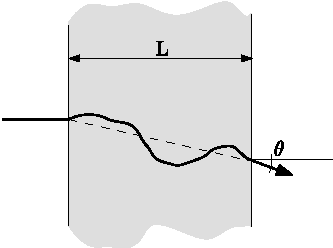
\includegraphics[width=0.78\columnwidth]{MultipleCoulombScat/MultipleScat.pdf}
    \caption{Left: Schematic representation of multiple coulomb scattering. Right: Schematic representation of electron backscattering.}
    \label{fig:PartScattering}
\end{figure}

It is very difficult to study any theory of multiple scattering for incident light particles such as electrons, due to the large number of scattering processes, not only by the atomic nuclei but also by the other electrons in the medium \parencite*[][]{ref:MultipleElec1}. Equation \ref{eq:multscat} is no longer valid in the case of a light particle \parencite*[][]{ref:MultipleElec2}, where large scattering angles are not rare. If an incident particle is scattered back of the material, it is called a backscattered particle. See figure \ref{fig:PartScattering} (right) for a schematic representation of the phenomenon.  Experimental information about this phenomenon has been intensively collected and from an empirical point of view, this phenomenon is well understood. However, attempts at a theoretical interpretation of the data have only limited success \parencite[][]{ref:BackScatTheo}.

For this document, we will only concern ourselves with the back-scattering electron yield ($BS_{el}$), which can be defined as the ratio between the number of outgoing primary electrons and the incident electron flux. Back-scattering of heavier particles, such as protons, is also possible. However, for our range of energies and materials, we consider this to be negligible.

\subsection{Path Length and Range}
\label{sec:Range}
The distance traveled by a particle inside a target until it loses all its energy can be quantified using the range. The range is an experimental concept, for which there are several definitions, all roughly relating to the same quantity \parencite*[][]{ref:Knoll}. In this document, the range (R) is defined as the penetration depth in a medium that reduces the number of incident particles to one-half. The maximum penetration depth ($R_{max}$) is defined as the depth in the absorbing medium beyond which no particles are observed to penetrate. Finally, the total path length describes the distance traveled by the particle measured along the actual path of the particle. Figure \ref{fig:RangeVsPathLength} illustrates the differences between these definitions. 

\begin{figure}[h]
    \centering
    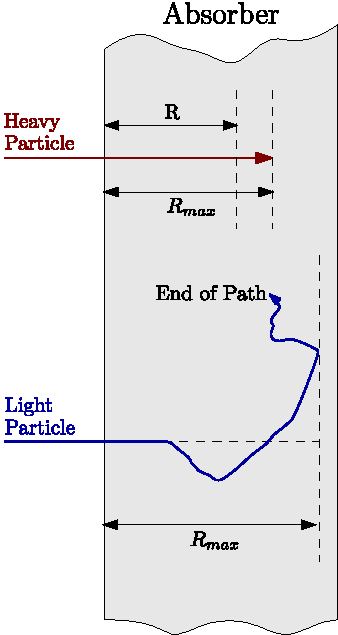
\includegraphics[width=0.9\columnwidth]{RangeVsPath/RangeVsPath.pdf}
    \caption{Schematic diagram of charged particle penetration into absorbing medium. Left: Heavy charged particle. Right: Light Charged particle.}
    \label{fig:RangeVsPathLength}
\end{figure}

The range highly depends on the type of particle, its energy and on the material through which it passes through. For a heavy particle that losses energy through ionization and atomic excitation, the range (R) can be calculated through the Continuous Slowing Down Approximation (CSDA): 

\begin{equation}
    R_{CSDA} = \int_{0}^{E_0} \left( \frac{dE}{dx} \right)^{-1} dE
    \label{eq:rangeCSDA}
\end{equation}

Where $E_0$ is the initial particle energy. This approximation assumes a smooth path, without hard collisions and large scattering angles. Some examples of analytical derivations of this equation can be found in \parencite*[][]{ref:CSDA}. The CSDA range for heavy non-relativistic charged particles, of mass $M_0$ and energy $E_k$, in a given absorber can be written in terms of the proton CSDA range ($R^{p}_{CSDA}$)as follows: 

\begin{equation}
    R_{CSDA}^{M_0} \left( E_K \right)= \frac{1}{Z^2} \left(\frac{M_0}{m_p}\right) R_{CSDA}^{p}\left[ E_K \frac{m_p}{M_0}\right]
\end{equation}

Where $M_p$ is the proton mass and Z is the atomic number of the incident ion. This can be very useful, as the range of protons in a variety of absorbers has been extensively measured. For heavy charged particles, $R_{max} \sim R_{CSDA}$ in all types of absorbing media. 

In the case of light particles, this CSDA approximation is not valid due to the very tortuous path that they experience in the absorbing medium. In this case, the CSDA range can be up to twice the average path for high Z absorbers ($R_{max} = 1/2 R_{CSDA}$). A useful quantity in the case of light particles is called the radiation length ($X_0$), usually measured in $g cm^2$. This gives us a mean distance over which high-energy particle losses all but $1/e$ of its energy by Bremsstrahlung. Different values for this quantity are available in literature, estimated with varying degrees of approximations. Some of these expressions can be found in \parencite*[][]{ref:radiationLength} and an example of an expression for high energetic electrons in high Z materials: 
\begin{equation}
    X_0 = \frac{716.405 A}{Z\left(Z+1\right)ln\left(183 Z^{-1/3}\right)}
    \label{eq:radiationlength.}
\end{equation}

\subsection{Types of Absorbers}

We will distinguish between thin and thick absorbers. In thin absorbers, only a few collisions of the projectile with the target atoms are likely to happen. Contrarily, in thick absorbers, a projectile experiences many collisions and the projectile energy lost by the incident particle is considerable. One can consider a target to be thin when the range of the incident particles is much larger than the thickness of the material ($R(E_k) >> L$). For thin absorbers, the energy loss is small and the stopping power doesn't change much along the length of the material. The total energy loss in the absorber can be calculated as: 

\begin{equation}
    \Delta E = - \left(\frac{dE}{dx}\right)_{avg} \cdot L
    \label{eq:thinabs}
\end{equation}

Here, the trajectory of the particle is also assumed to be perfectly linear in the absorber. If the range of the particles in the material is comparable to the thickness or smaller, this approximation is no longer valid, as one would underestimate the real energy deposition in the material. The energy is lost, the probability of interactions with the absorber material increases, since the ionization interaction cross-sections are bigger for smaller energies. A plot representing the specific energy loss along the incident particle track is called the Bragg curve. Figure \ref{fig:Bragg} shows an example of Bragg curve in the case of 3 \si[]{\mega\electronvolt} protons in graphite. 

\begin{figure}[h]
    \centering
    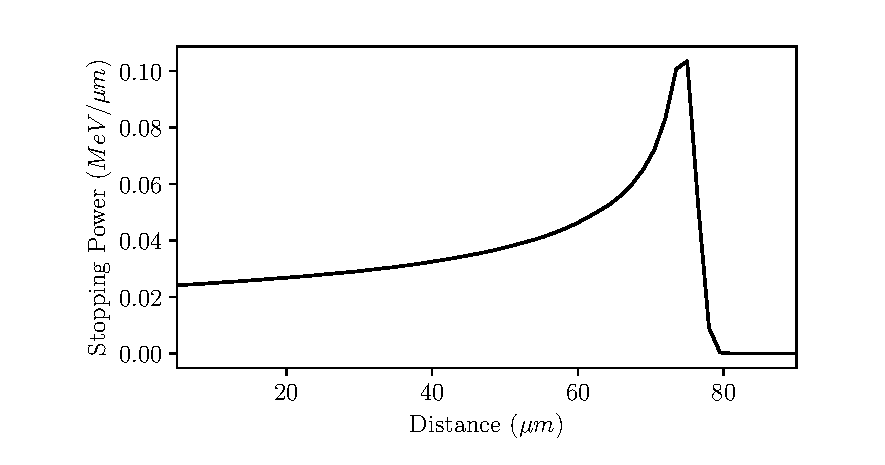
\includegraphics[width=1.0\columnwidth]{Bragg_Graphite/Bragg.pdf}
    \caption{Bragg peak of 3 \si[]{\mega \electronvolt} protons in Graphite. }
    \label{fig:Bragg}
\end{figure}

\section{Secondary Electron Theory}
\label{sec:SEY}
When a particle passes through the interface of a material, it will transfer energy to the electrons in the medium. Depending on the energy these electrons get, they can be excited to a higher energy level, or gain enough energy to be emitted from the material, this emission
process is known as Secondary Electron Emission (SEE) \parencite*[][]{ref:see1}. The SEE process can be generally divided into three consecutive steps:

\begin{enumerate}
    \item Generation Process: The energy required to ionize the atoms in the material is the minimum energy needed to create a secondary electron (SE). If the incident projectile is an ion containing electrons, these electrons can also be stripped off and produce further ionization. However, if the electrons from the incident ions are scattered off the material, they cannot be counted as secondary electrons. 
    \item Diffusion Process: While the SE travel through the material, they lose energy. This energy loss permits only a very shallow penetration depth of the low-energy electrons. For that reason, SE tends to be a surface phenomenon. 
    \item Emission Process: To be emitted from the surface, the SEs have to overcome the surface barrier potential \parencite*[][]{ref:see2}. The escape process is of particular importance because it determines the final shape of the secondary electron distribution. Moreover, the velocity vector, when reaching the surface, must allow the SE to escape. In the case of metals and semiconductors, a cosine-type angular distribution of SE is observed \parencite[][]{ref:angleSemi}
\end{enumerate}

\begin{figure}[h]
    \centering
    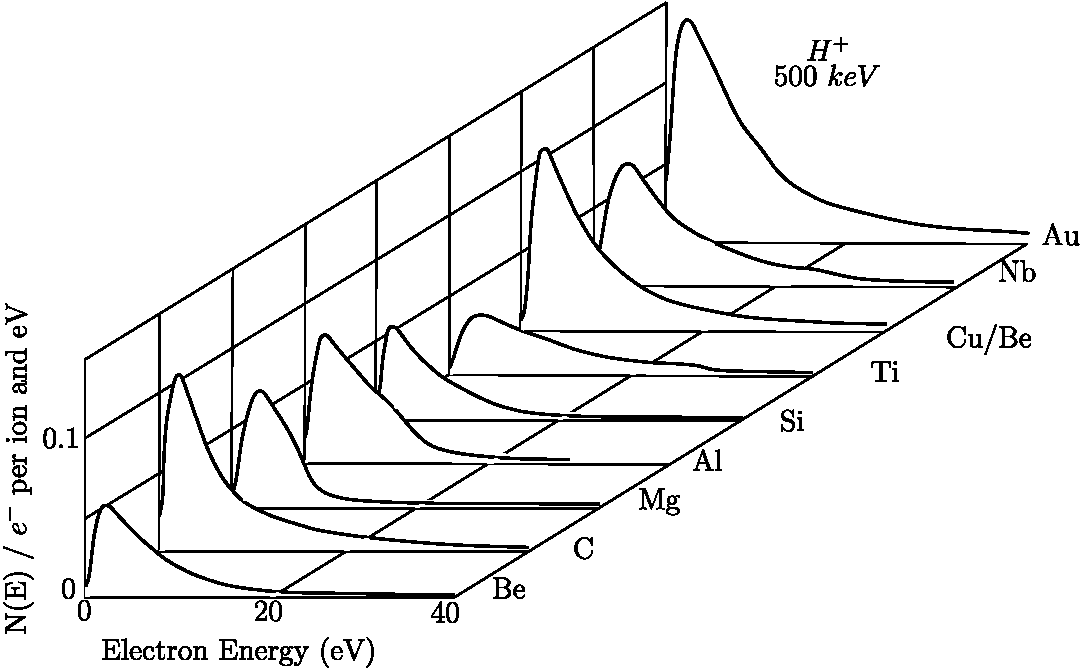
\includegraphics[width=0.9\columnwidth]{SEE_Spectra/SeeSpectra.pdf}
    \caption{Ion induced secondary electron spectra for a variety of metals. Incident ion: Proton 500 \si[]{\kilo \electronvolt}. From \parencite*[][]{ref:SEEspectra} }
    \label{fig:MetalsSE}
\end{figure}

Many experimental measurements of secondary electrons have been done since the discovery of this phenomenon in 1902, revealing some commonalities: In the case of SEE from metal surfaces \parencite*[][]{ref:see3},  The energy spectra of SE peak at about 1-5 eV; The full width of the peak is around 3-15 \si[]{\electronvolt}; It is commonly said that SE, in general, have an energy $< 50$ \si[]{\electronvolt}. Figure \ref{fig:MetalsSE} shows the spectra of SE emitted from different metals for an incident 500 \si[]{\kilo\electronvolt} proton. 

The main parameter describing the SEE is the Secondary Emission Yield (SEY). It describes the average number of electrons emitted per incident projectile. A semi-empirical treatment of SEY was formulated by E.J. Sternglass in 1957 \parencite*[][]{ref:SEY}. In this formulation, two sources of SE are considered. Firstly, the SE generated by small energy transfers from the incident particles to the target electrons. This first mechanism is the main contributor to the SEY. Secondly, a smaller contribution comes from the SE generated by delta electrons (defined in the following section). This formulation allows for the following numerical relation: 

\begin{equation}
    SEY = 0.01 L_S \left. \frac{dE}{dx}\right|_{el} \left[ 1+\frac{1}{1+5.4\cdot 10^{-6} E/A_p}\right]
    \label{eq:sey}
\end{equation}
\begin{equation}
    L_S = \left( 3.68\cdot 10^{-17} N_v Z^{1/3} \right)^{-1}
    \label{eq:LS}
\end{equation}

Here, E and $A_p$ are the kinetic energy and the mass of the projectile. $L_{s}$ is the characteristic length, which is of the order of the distance between inelastic collisions, and it is expressed in (\si[]{\centi\metre}). $N_v$ is the number of atoms per unit volume. $dE/dx$ is the energy deposition in the material due to interactions with the electrons. It should be expressed in eV/cm. As we saw previously (subsection\ref{sec:Bethe}), this term is greatly affected by the speed of the incident particle and its nature. 

The Secondary Emission Yield also depends on the angle of incidence of the incident particle. In the theory of Sternglass, the angular dependence is treated as a change in the effective penetration distance $L_{s}$. If the particle impacts at an angle different to the normal, the effective track length of the projectile extends by a factor $1/cos(\theta)$. In that case the corresponding SEY would be: 

\begin{equation}
    \frac{SEY(\theta)}{SEY(0)} = \frac{1}{cos(\theta)}
\end{equation}

Experimental values confirm this approximation for incident angles up to $70\deg$. However, if the incident particles are electrons, recent measurements show a different angular dependence \parencite*[][]{ref:seyAngleEl}: 
\begin{equation}
    \frac{SEY(\theta)}{SEY(0)} = e^{0.5 \left(1-cos(\theta)\right)}
\end{equation}

Early investigations of SEE already show a dependence of SEE on temperature \parencite*[][]{ref:SeyVsTemp}. Temperature seems to affect the escape probability. An increase in temperature results in increased vibrations of the atoms about their equilibrium position, which should reduce $L_{s}$, therefore increasing the Yield. Sternglass gives a rough quantitative hypothesis that goes as follows: 
\begin{equation}
    \frac{L_S (T_1)}{L_S(T_2)} = \frac{1+2.5\cdot 10^{-3}T_1}{1+2.5\cdot 10^{-3}T_2}
\end{equation}

Where $L_{S}(T_{1})$ is the characteristic length at $T_{1}$ and $L_{1}(T_{2})$ is the length at $T_{2}$. It is important to note that the semiempirical theory of secondary emission is only considered to be accurate for backward emission (projectile entering the target). As a first approximation, here we will consider that this formulation is also valid for rear-face emission. 

\subsection{Delta Rays}

Most frequently, the electrons generated by SE have low energy. However, if the energy transferred to the electron is above a few hundred \si[]{\electronvolt} (up to $T_{max}$), they might be able to generate further ionization on their own. An analytical formulation for the total number of $\delta$-rays produced from charged particle interactions was presented by Rossi in 1952 \parencite*[][]{ref:delta1}, and gives the distribution of $\delta$ rays for incident particles with energy $I \ll T \ll T_{max}$ as follows: 
\begin{equation}
    \frac{d^2N_{\delta}}{dTdx} = \frac{1}{2}Kz^2\frac{Z}{A}\frac{1}{\beta^2}\frac{F(T)}{T^2}
    \label{eq:deltaN}
\end{equation}

Where $T_{max}$ is given by equation \ref{eq:tmax}. The factor F is spin-dependent, but it is about unity for $ T \ll  T_{max}$. To calculate the total number of generated delta rays per unit of distance, one can integrate the previous equation from an arbitrary lower limit to the maximum energy for delta rays can get ($T_{max}$), described by Eq. \ref{eq:tmax}. 



\chapter{Signal Generation Simulations} 
\label{ch:CurrentModeling}
\pagestyle{fancy}

\graphicspath{ {Figures/Chapter3_IntensitySimulation/} }

In this chapter, the signal generation in secondary emission monitors (SEM) when traversed by a particle beam will be covered. The formulations are going to be rather broad, for a generic particle beam and energy range. However, all the numerical examples will refer to SEM grids and Wire Scanner detectors in LINAC4. 

\section{Signal Generation in SEM}

At first, one can define the net charge generated on a wire or a foil transversed by a particle projectile (Proj) as: 

\begin{equation}
    \label{eq:Qsum}
    Q\left(\frac{e}{Proj}\right) = Q_{dep} + Q_{SE} + Q_{th}
\end{equation}

Where $Q_{dep}$ represents the charge generation due to Charge deposition. $Q_{SE}$ is the charge due to secondary emission and $Q_{th}$ is the charge due to thermionic emission. Figure \ref{fig:SignalGeneration} shows a schematic representation of the different processes that contribute to the charge generation in the material. They will be detaidely covered in the next sections. 

\begin{figure}[h]
    \centering
    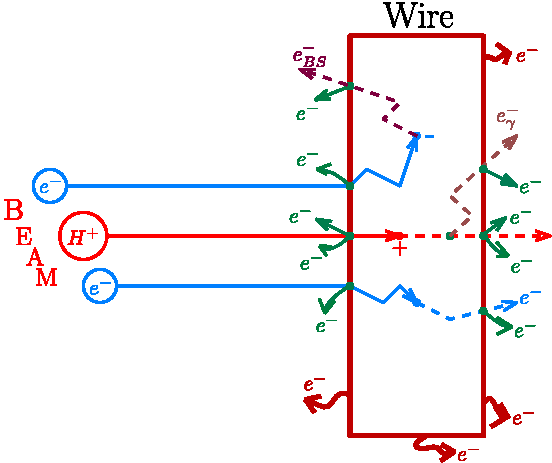
\includegraphics[width=0.50\columnwidth]{Figure_ChargeGeneration/ChargeGen.pdf}
    \caption{Schematic Representation of processes inducing current in the detector material.}
    \label{fig:SignalGeneration}
\end{figure}

\subsection{Charge Deposition ($Q_{dep}$)}

When an ion with $N_p$ number of protons in the nucleus and $N_e$ non-stripped electrons hits a target, the electrical charge directly deposited in the target depends on the probability of the protons and the electrons remaining on it. This can be written as: 

\begin{equation}
    Q_{dep} = N_p \cdot \eta - N_{e}\cdot \mu
\end{equation}

Where $\eta$ is the proportion of protons that are stopped in the material and $\mu$ is the proportion of electrons. These parameters depend on the range of the particles in the detector material, which was described in \ref{sec:Range}, and on the back-scattering probability, explained in \ref{sec:BS}. 

\subsection{Secondary Emission Charge ($Q_{SE}$)} 

The charge generated in the material by a particle, with $N_p$ number of protons and $N_e$ number of electrons, can be modeled as: 

\begin{equation}
    \begin{split}
        Q_{SE} = N_p \cdot SEY_{p1} + N_p \left(1-\eta\right)SEY_{p2} + 
                N_e \cdot SEY_{e1} + N_e \left( 1 - \mu \right) SEY_{e2} + \\
                N_p \cdot BS_p \cdot SEY_{BSp} + N_e \cdot BS_e \cdot SEY_{BSe}
    \end{split}
    \label{eq:Qse}
\end{equation}

Secondary emission is a surface process. In the case of a thin target detector, SE can occur at the entrance surface ($SEY_1$) and at the exiting one ($SEY_2$). And it can be induced by both the incident protons ($SEY_p$) and the electrons ($SEY_e$). In some cases, the probability of electron and proton backcattering ($BS_e$ and $BS_p$) is not negligible. In those cases, one must also consider the contribution of the secondary electrons generated due to the backscattered particles crossing twice the incident surface ($SEY_{BEp}$ and $SEY_{BEe}$).

In all the cases, SEY represents the secondary emission yield that was introduced in \ref{sec:SEY}. As was mentioned in the previous chapter, the semi empirical formula for secondary emission is valid at the entering surface as it does not account for energy loss in the material. For this reason in equation \ref{eq:Qse}, we specified the entrance surface as 1 and the exit surface as 2. One could try to obtain a more accurate description of the SE at the exit surface by accounting for the energy loss in the material. 

Similarly occurs with the back-scattering case. Backscattered particles might have different incident and exiting energies. If so,  $SEY_{BS}$ can be calculated more accurately. However, properly calculating the energy deposition induces some complications that, in some cases, might not be rewarded with a tangible improvement. 

\subsection{Thermionic Emissioon Charge ($Q_{Th}$)}
\label{sec:ThermoCurrent}
Thermionic emission is the process by which free electrons are emitted from the surface of a metal when they gain enough thermal energy to overcome the work function. As thermionic electrons are negative charges exiting the material surface, they will contribute to signal generation. $J_{Th}$ is the current density of emitted electrons and it is described by Richardson-Duschman equation \parencite[][]{ref:Richardson}:

\begin{equation}
    J_{Th} = A_R \cdot T^2 \cdot exp\left(-\frac{\phi}{k_B T} \right) 
    \label{eq:ThermoCurrent}
\end{equation}

$A_R$ is the Richardson constant and $K_B$ is Boltzmann's constant. From this equation, one can observe how dependent thermionic emission is on temperature. It is not until high temperatures are reached that thermionic emission can be detected. More on this will be explained in the following chapters. 

\section{LINAC4 Signal Generation Studies.}

As was introduced in \ref{sec:LINAC4}, LINAC4 accelerates \hm particles up to 160 MeV. \hm ions consist of one proton ($N_p$ = 1) and two electrons ($N_e$ = 2). In this case formula \ref{eq:Qsum} can be written as: 

\begin{equation}
    Q\left(\frac{e}{H^{-}}\right) = \eta - 2\mu + \left( 2 - \eta + BS_p \right) \cdot SEY_p +2\left( 2 - \mu - BS_e \right) \cdot SEY_e
    \label{eq:Ql4}
\end{equation}

Note that in this case, we are considering the secondary emission yield for electrons and protons to be the same at the entrance and the exit of the detectors. As we will see in the following, this might not be the most accurate procedure for some of the detectors at LINAC4. Figure \ref{fig:RangeLinac4} shows how the values of the range of protons change as a function of the particle energy. 

\begin{figure}[h]
    \centering
    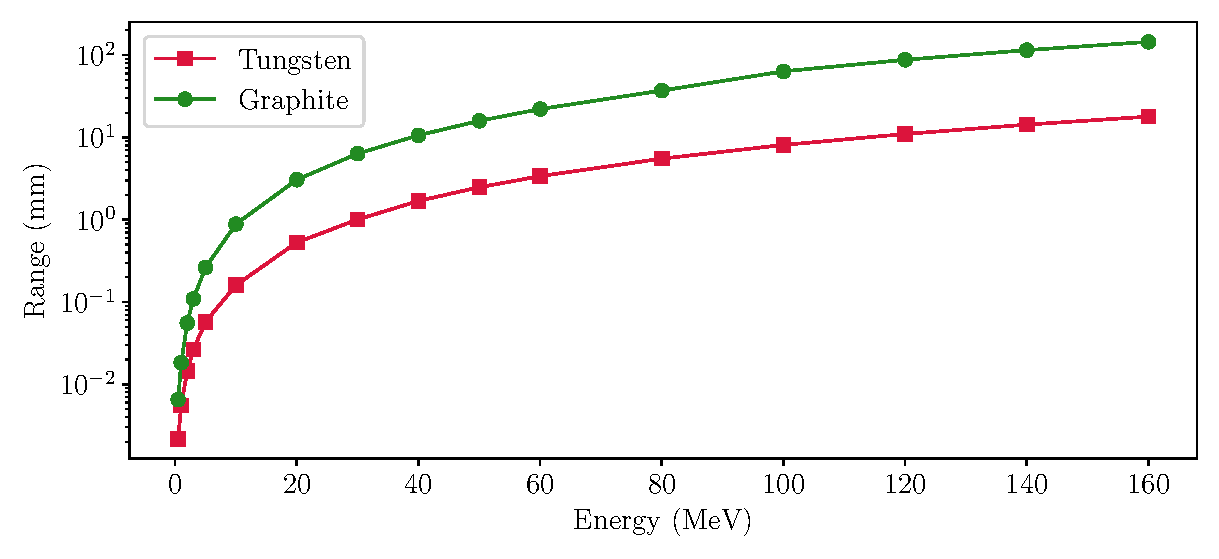
\includegraphics[width=0.9\columnwidth]{RangePlotLinac4/RangeL4.pdf}
    \caption{Range of particles as a function of incident ion energy.}
    \label{fig:RangeLinac4}
\end{figure}

From this figure, we can see how the range of the particles in the material increases as their energy increases. For the same energies, the particles have a much larger range in the case of graphite compared to tungsten. At LINAC4, the wires have a width of $40$ \si{\micro\metre} for the case of tungsten and 33 \si{\micro \metre} for the case of graphite wires. 

The range of protons is larger than the detector thickness in most of the energy range. Only tungsten detectors placed at energies smaller than 5  \si[]{\mega\electronvolt} are expected to get a positive charge deposition. The electrons in an \hm ion have energy much smaller than the proton. It is actually reduced a factor $m_p / m_e = 1836.15$ compared to the energy of the \hm ions.  Electrons are expected to deposit all their energy in all the SEM grids and Wire scanners at Linac4. So we expect to always have a double negative charge contribution. 

Table \ref{tab:ChargePar} summarizes the values for $\eta$ and $\mu$ parameters along the Linac4 accelerator range. This table also summarizes the values of the Backscattering probabilities for both electrons and protons. All these values have been calculated with Geant4 \parencite[][]{ref:Geant4}. The backscattering probability is negligible for the protons. Contrarily, electron backscattering probability is not negligible. In the case of tungsten, for ion energies of 160 MeV half of the electrons are backscattered.

% Please add the following required packages to your document preamble:
% \usepackage{multirow}
\begin{table}[h]
    \begin{tabular}{cccccccccc}
    \hline
    \multirow{2}{*}{\begin{tabular}[c]{@{}c@{}}$p^+$ energy \\ (MeV)\end{tabular}} & \multirow{2}{*}{\begin{tabular}[c]{@{}c@{}}$e^-$ energy\\ (keV)\end{tabular}} & \multicolumn{4}{c}{Graphite} & \multicolumn{4}{c}{Tungsten} \\ \cline{3-10}  &   & $\eta$   & $\mu$     & $BS_p$ & $BS_e$   & $\eta$ & $\mu$     & $BS_p$ & $BS_e$     \\ \hline
    3                                                                     & 1.63                                                                           & 0.001 & 0.918 & 0.0 & 0.081 & 1.0 & 0.632  & 0.0 & 0.367   \\
    50                                                                    & 27.23                                                                          & 0.0   & 0.931  & 0.0 & 0.068 & 0.0 & 0.506  & 0.0 & 0.493  \\
    102                                                                   & 55.55                                                                          & 0.0   & 0.887  & 0.0 & 0.112 & 0.0 & 0.487 & 0.0 & 0.512 \\
    160                                                                   & 87.14                                                                          & 0.0   & 0.857  & 0.0 & 0.142 & 0.0 & 0.464  & 0.0 & 0.536   \\ \hline
    \end{tabular}
    
    \caption{Summary of charge deposition and backscattering probabilities for Tungsten ($40 \mu m$) and Graphite ($33 \mu m$)} detectors.
    \label{tab:ChargePar}
\end{table}

Figure \ref{fig:SEYmat} shows the Secondary Emission yield calculated with the semiempirical Sternglass formula (Eq. \ref{eq:sey}) as a function of the incident proton energy.  In both materials, the SEY reaches a maximum ( $~ 0.1 $ MeV ) which is followed by a decrease in the SEY. Graphite presents a higher SEY at smaller proton energies whereas tungsten presents a higher SEY at higher incident particle eneriges. 

\begin{figure}[h]
    \centering
    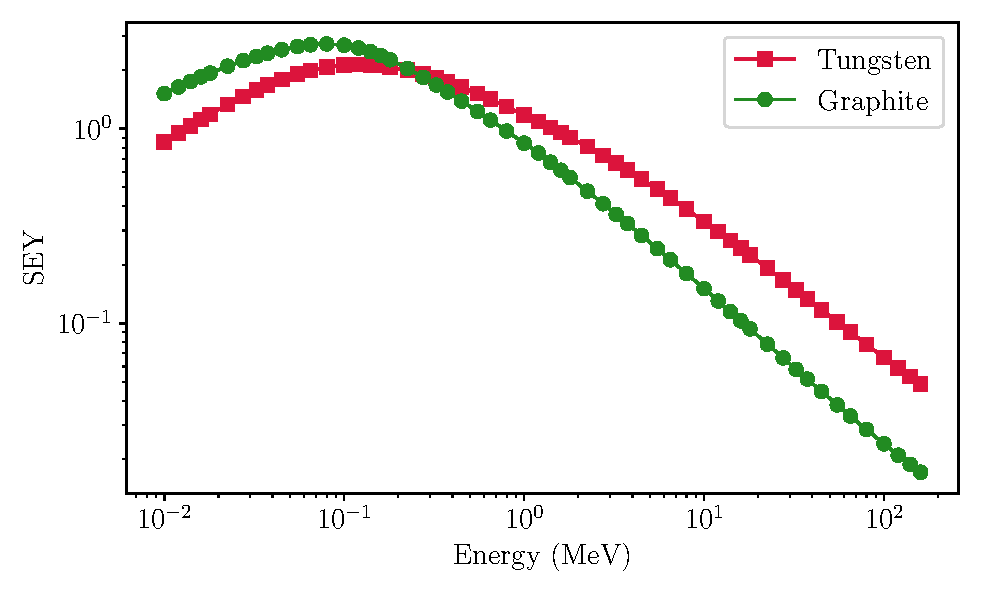
\includegraphics[width=0.85\columnwidth]{Figure_SEY/SEY_compa.pdf}
    \caption{Secondary Emission Yield as a function of incident proton energy. }
    \label{fig:SEYmat}
\end{figure}

As an example, figure \ref{fig:ProfComparison} shows a simulated beam profile at 3 MeV and 160 MeV. From these figures, we can observe how at 3 (MeV) the positive contribution to the charge is predominant for the case of tungsten wires while it remains negative in the case of graphite wires. Due to the smaller SEY of graphite at 160 (MeV), the absolute registered signal at this energy is higher than the one registered by the tungsten wires. 

\begin{figure}[h]
    \centering
    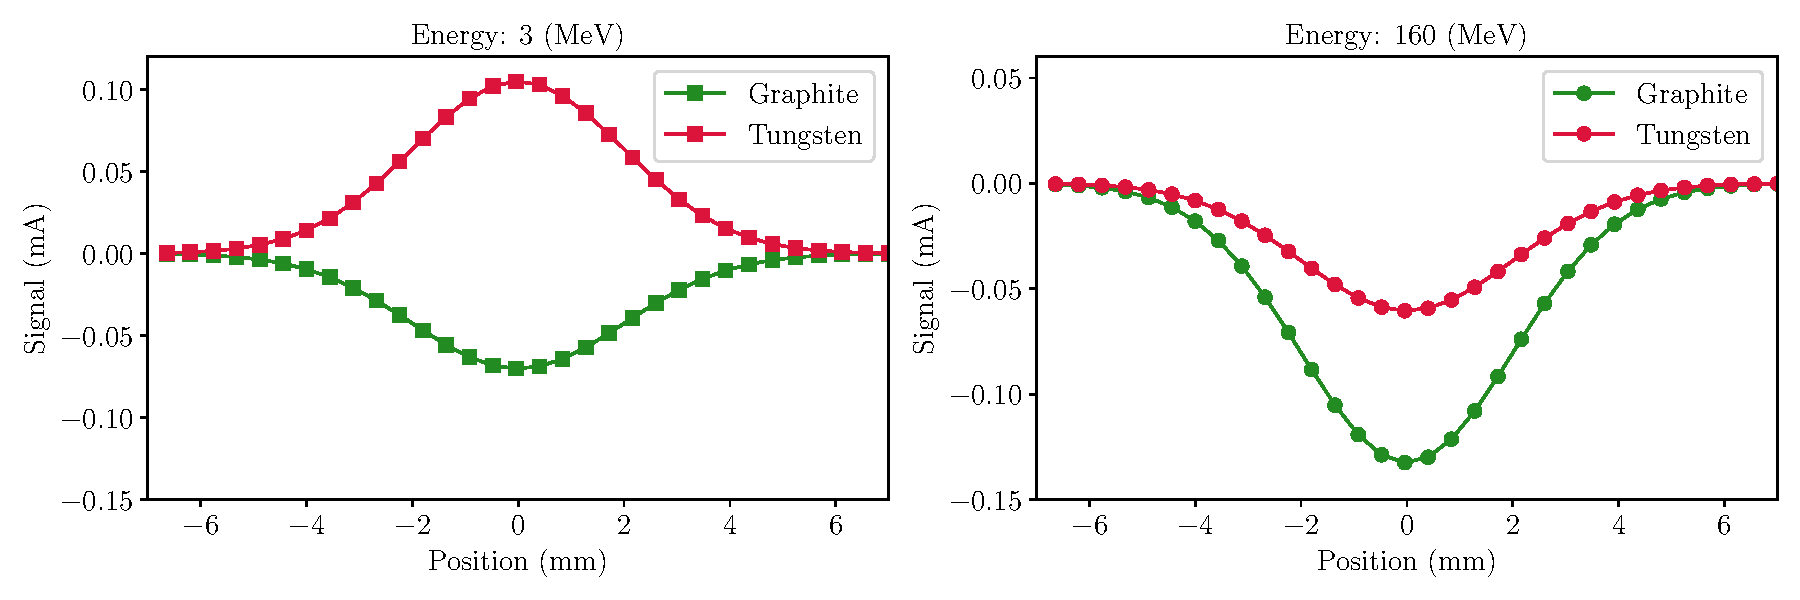
\includegraphics[width=0.85\columnwidth]{Figure_ProfCompa/ProfileComparison.pdf}
    \caption{Expected transverse beam profile for incident \hm particles. Left: 3 (MeV), Right: 160 (MeV). For these simulations, a 25 mA, 100 $\mu s$ particle beam was considered. }
    \label{fig:ProfComparison}
\end{figure}

At Linac4, even if these detectors are called Secondary Emission Monitors, the biggest contribution to the charge formation is the charge deposition term. To prevent misinterpretations, SE is typically suppressed by a bias current.  At LINAC4, the detectors at lower energies are usually conformed with graphite wires, to avoid the positive contribution of the proton charge deposition. 

\section{Beam Intensity and Profile Measurements at CERN LINAC4.}

In this section, we will briefly show how the instruments just presented are used at CERN, LINAC4. All the results presented in this section correspond to the first profile and current measurements for the LBE run, which took place in November 2019 \parencite*[][]{ref:PresentationLBERun}. The objective of these measurements was to study the transverse profile evolution of the particle beam along the LINAC4 accelerator. 

Figure \ref{fig:Linac4Layout} shows a schematic representation of LINAC4 with the different detectors and locations. In this figure, the yellow circles represent the BCTs. The blue and red rectangles indicate the positions of SEM grids and Wire scanners respectively. Green rectangles indicate positions where SEM grid and Wire scanners are installed at the same position. As we can see from this figure, both BCTs and Beam profile instruments are placed all along LINAC4 so the beam parameters can be measured in all the acceleration stages. 

\begin{figure}[h]
    \centering
    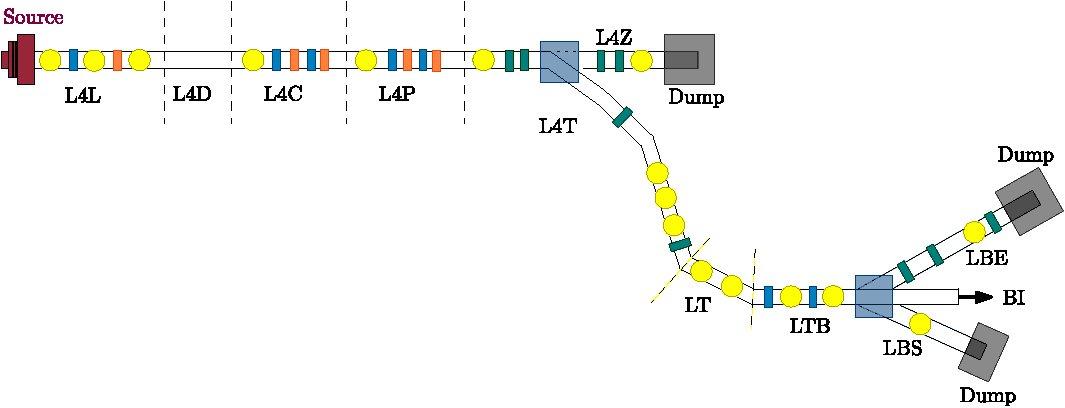
\includegraphics[width=1.0\columnwidth]{Linac4Instrumetnation/Linac4Instruments.pdf}
    \caption{Schematic representation of LINAC4 with the location of some diagnostics devices.}
    \label{fig:Linac4Layout}
\end{figure}

Figure \ref{fig:BCTwithTime} shows an example of intensity measurement taken by the first BCT in the L4T segment. From this figure, one can identify the beam pulse, we can observe that due to the accelerator of $H^{-}$ particles at LINAC4, the registered current is negative. In this case, the beam pulse length was 36 \si[]{\micro \second} with an average intensity of $\sim 17 $ \si[]{\milli \ampere}. One can observe the 1 \si[]{\micro \second} gaps generated by the chopper, which make the beam pulse ready to be injected into the different pulse rings. 

\begin{figure}
    \centering
    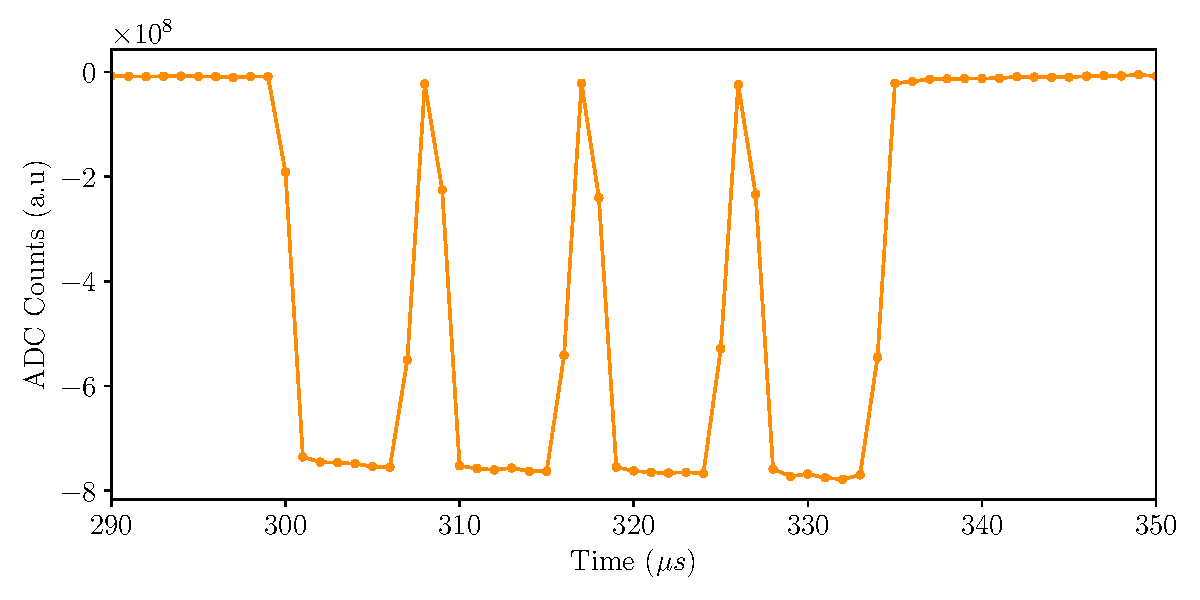
\includegraphics[width=0.7\columnwidth]{IntensityVStime/IntensityVStime.pdf}
    \caption[The LOF caption]{Beam current shape along beam pulse, from first BCT in L4T line.}
    \label{fig:BCTwithTime}
\end{figure}

By measuring the average current of the beam at all the available BCTs, one can assess the beam transmission along the accelerator. Figure \ref{fig:BeamTrans} shows an example of beam transmission measured along the accelerator. From this figure one can observe how in all parts of the accelerator, except for the first two BCTs in the L4L line, the current remains quite constant around $\sim 17$ \si[]{\milli \ampere}.  Similarly, the beam transmission remains very close to $100 \%$ along the whole accelerator. 

\begin{figure}
    \centering
    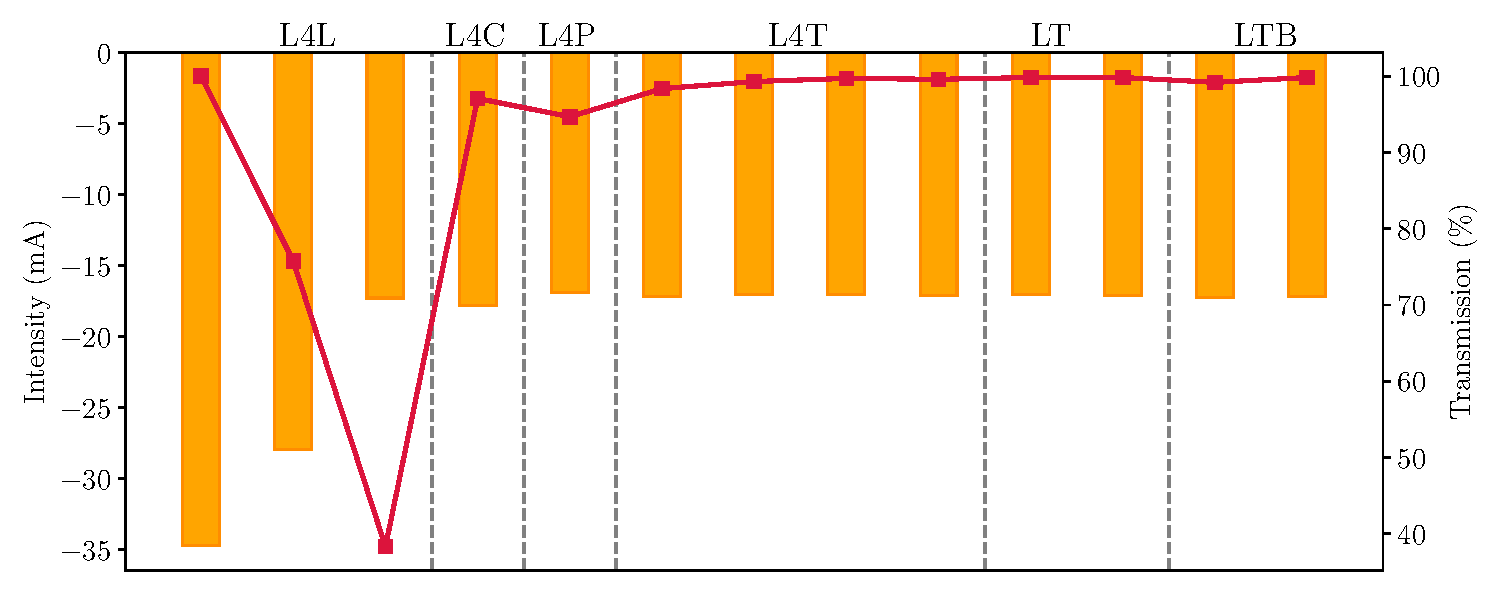
\includegraphics[width=0.9\columnwidth]{BCT_Transmission/TransmissionBCT.pdf}
    \caption{Average intensity measured by the different BCTs at LINAC4. Transmission along the LBE line.}
    \label{fig:BeamTrans}
\end{figure}


Similarly, the beam profile was measured along the accelerator, to cross-check the beam evolution as well as to assess the integrity and status of the devices installed along the accelerator.  Figure \ref{fig:HorizontalProf} shows the measurements of the horizontal profile of the beam along the LINAC4 accelerator. All these measurements were taken with the SEM grids. From this figure we can observe:

\begin{figure}
    \centering
    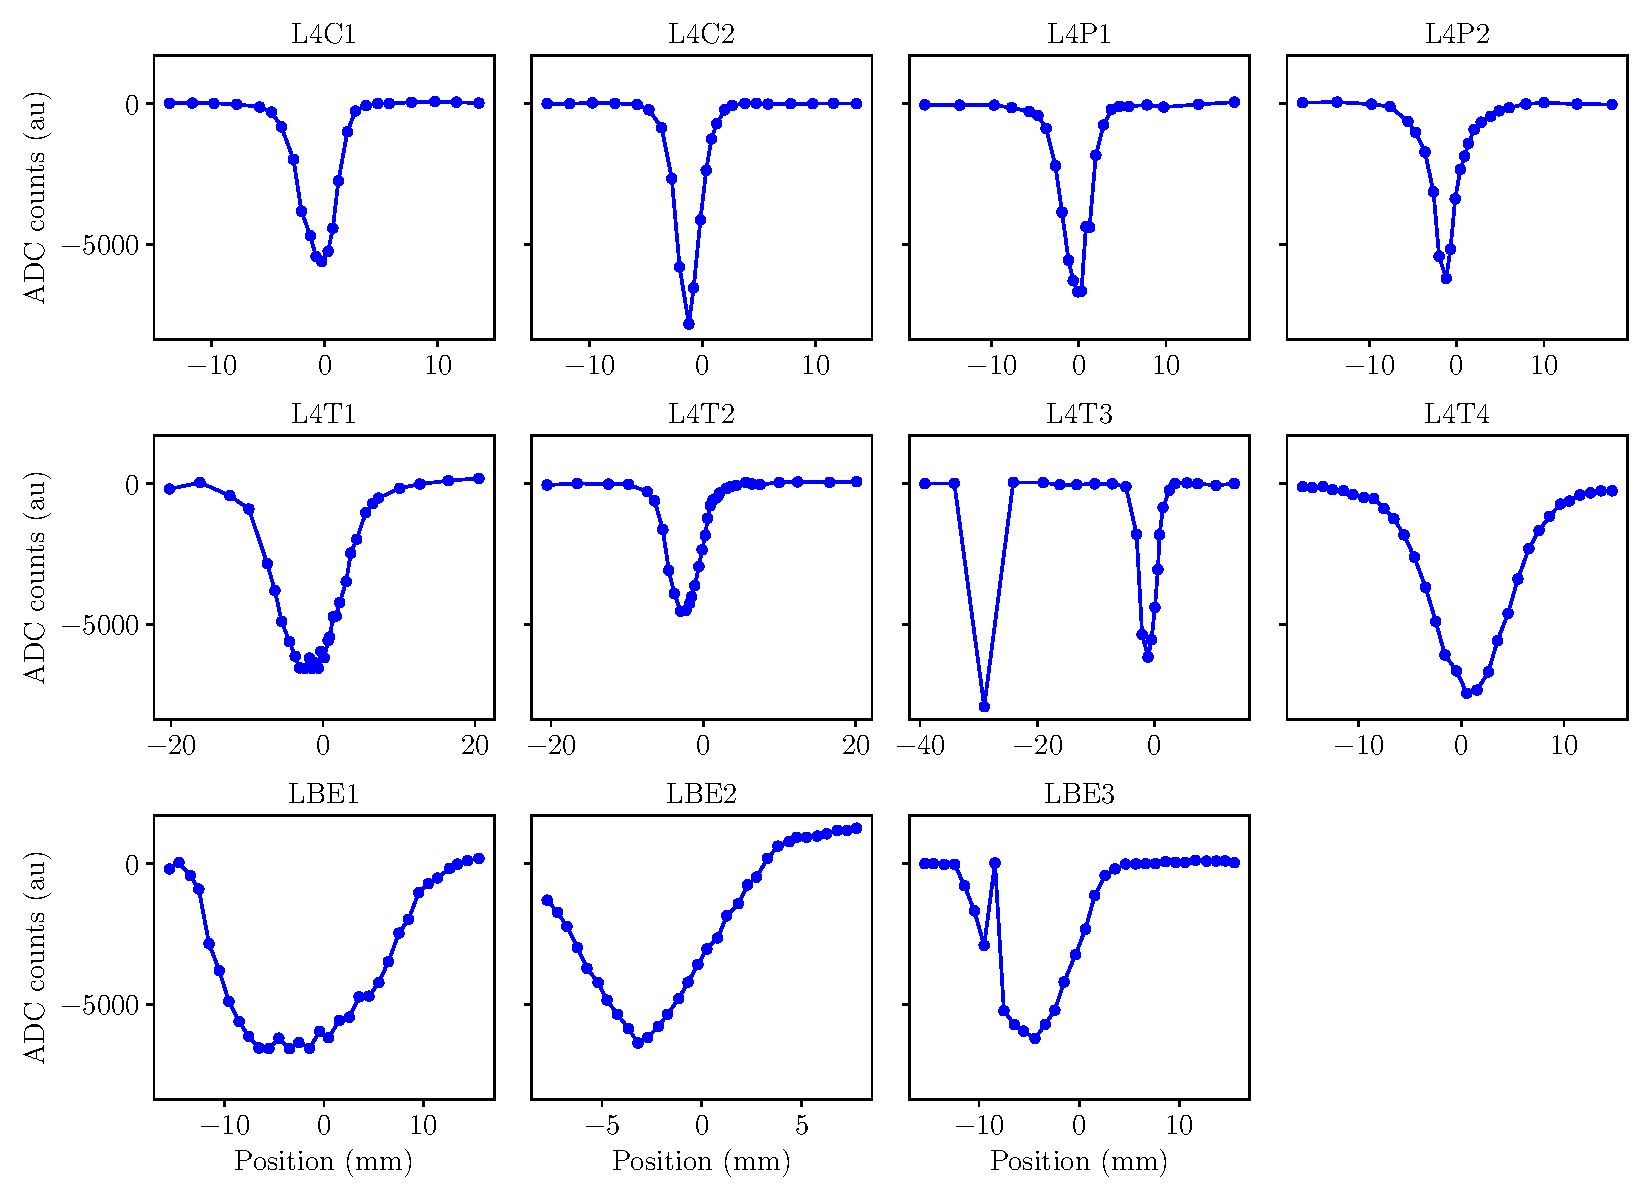
\includegraphics[width=1.0\columnwidth]{SigmaEvol/HorEvol.pdf}
    \caption{Horizontal transversal beam profile measured by the differt detectors at LINAC4}
    \label{fig:HorizontalProf}
\end{figure}

\begin{itemize}
    \item The beam profile seemed to be very much gaussian in all the measurement points except for LBE1 and LBE2 positions.
    \item Broken wires: SEM grids L4T2 and LBE3 present a broken wire that must be repaired. Wires 12-13 and 14-15 in L4P1 are glued together. 
    \item L4T1 and LBE1 present strange strange oscillations in the wires measuring the highest intensities. 
    \item Some of the grids have an even wire separation while others present a noneven wire distancing. Due to the beam not always being centered having smaller wire separation at the center of the grid des not seem to be that helpful.
    \item Not depicted, however, the data acquisition system for the detectors in the LBE sector had to be corrected to properly acquire the data.
\end{itemize}

Here we presented only the evolution of the horizontal profile, however, the evolution of the vertical profile was similarly studied. In the case of the vertical profile, a non-gaussian beam was observed in some of the locations. Figure \ref{fig:VertProf} shows an example of a vertical profile taken with both the second SEM grid and the second Wire Scanner from the L4T line. In this case, the particle beam clearly shows some shoulders or tails that push it away from the gaussian distribution. Another thing that one can observe from this figure, is the great agreement between the beam profile measurements by the sem grid and the wire scanner. 


These measurements were the first systematic set of measurements of the LBE run, they helped understand the beam evolution along the accelerator and thus helped correct the observed irregularities. These measurements also helped assess and correct any issue on the measuring devices, such as broken wires, position misreadings, data acquisition problems, etc.  

\begin{figure}[h]
    \centering
    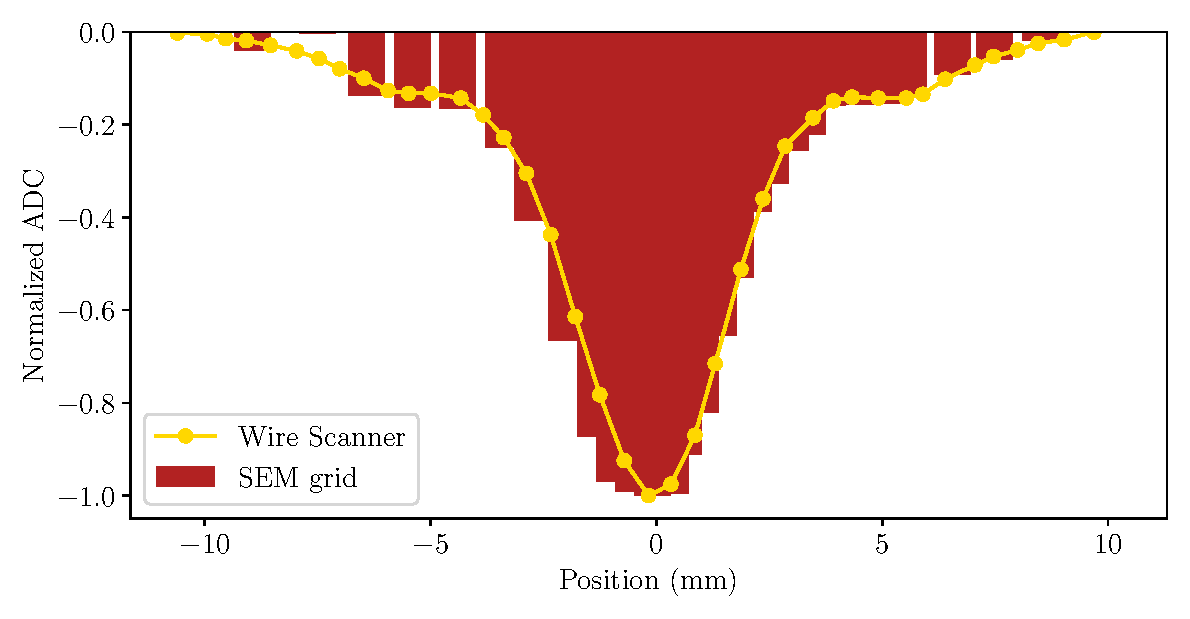
\includegraphics[width=0.6\columnwidth]{VertProf/VertProf.pdf}
    \caption{Vertical transverse profile measured by the second SEM grid and second wire scanner of the L4T line at Linac4.}
    \label{fig:VertProf}
\end{figure}






\chapter{Numerical Methods, Thermal Model.}
\label{ch:TempModeling}
\pagestyle{fancy}

\graphicspath{ {Figures/Chapter4_ThermalModel/} }

The bulk of this thesis consisted in implementing a thermal simulation code able to reproduce the thermal evolution of thin target detectors during operation.
The program implemented by M. Sapinski in 2012 for fast wire scanner simulations \parencite[][]{ref:Msapinski} was taken as a starting point. The idea started by M. Sapinski has been generalized to other types of thin target detectors, such as SEM grids, slow wire scanners and foils. Conduction cooling effects modeling has undergone a substantial update. Additionally, a (Graphical User Interface) GUI  has been implemented to facilitate the program's usage. 


\section{Introduction}

During operation, interceptive devices interact directly with the beam of particles. As was discussed in chapter \ref{ch:BeamMatterInter}, the beam of particles will deposit some energy in the detector's material. How much energy is deposited will depend on the beam energy, type of particle but also material detector and geometry. This deposited energy leads to a fast increase of the detector temperature. Depending on the beam conditions, the thermal shock suffered by the detectors can be very severe. This might affect the measured currents (Thermionic Emission), or in some cases permanently manage the detectors. 

\begin{figure}[h]
    \centering
    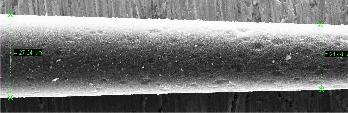
\includegraphics[width=0.60\columnwidth]{WireRadiusDeterioration/WireDamage.png}
    \caption{Carbon fiber wire scanner used at SPS in 2008.}
    \label{fig:WireRadius}
\end{figure}

At CERN, $34 \mu m$ carbon fiber wire scanners are used. Because of high brightness of proton and ion beams, the fibers are moved at high
speeds, between 1 and 6 m/s. Despite that, scanning is not possible at certain beam conditions, for instance at full LHC intensity, due to wire damage. Figure \ref{fig:WireRadius} shows a picture of a wire scanner photographed with a scanning electron microscope. This scanner was used in 2008 at CERN SPS during a systematic breakage experiment \parencite[][]{ref:Msapinski}. This picture shows how the radius of the wire was reduced due to the sublimation process after consecutively reaching high temperatures.

Another clear example of detector damage due to high temperature can be observed in Figure \ref{fig:SEMLinac4damage}. In this case, we can observe three pictures taken from a SEM grid used at LINAC4 in 2019. This grid had $40 \mu m$ gold-coated tungsten wires. Already in the first picture (left) we can observe how the gold coating was evaporated from the wires in the central part of the grid (Gold Melting Temperature is ~ 1400 K). From the images taken with the optical microscope (center), we can observe two wires glued together due to the high temperatures reached by the detector. 

\begin{figure}[h]
    \centering
    \begin{subfigure}[b]{0.42\textwidth}
        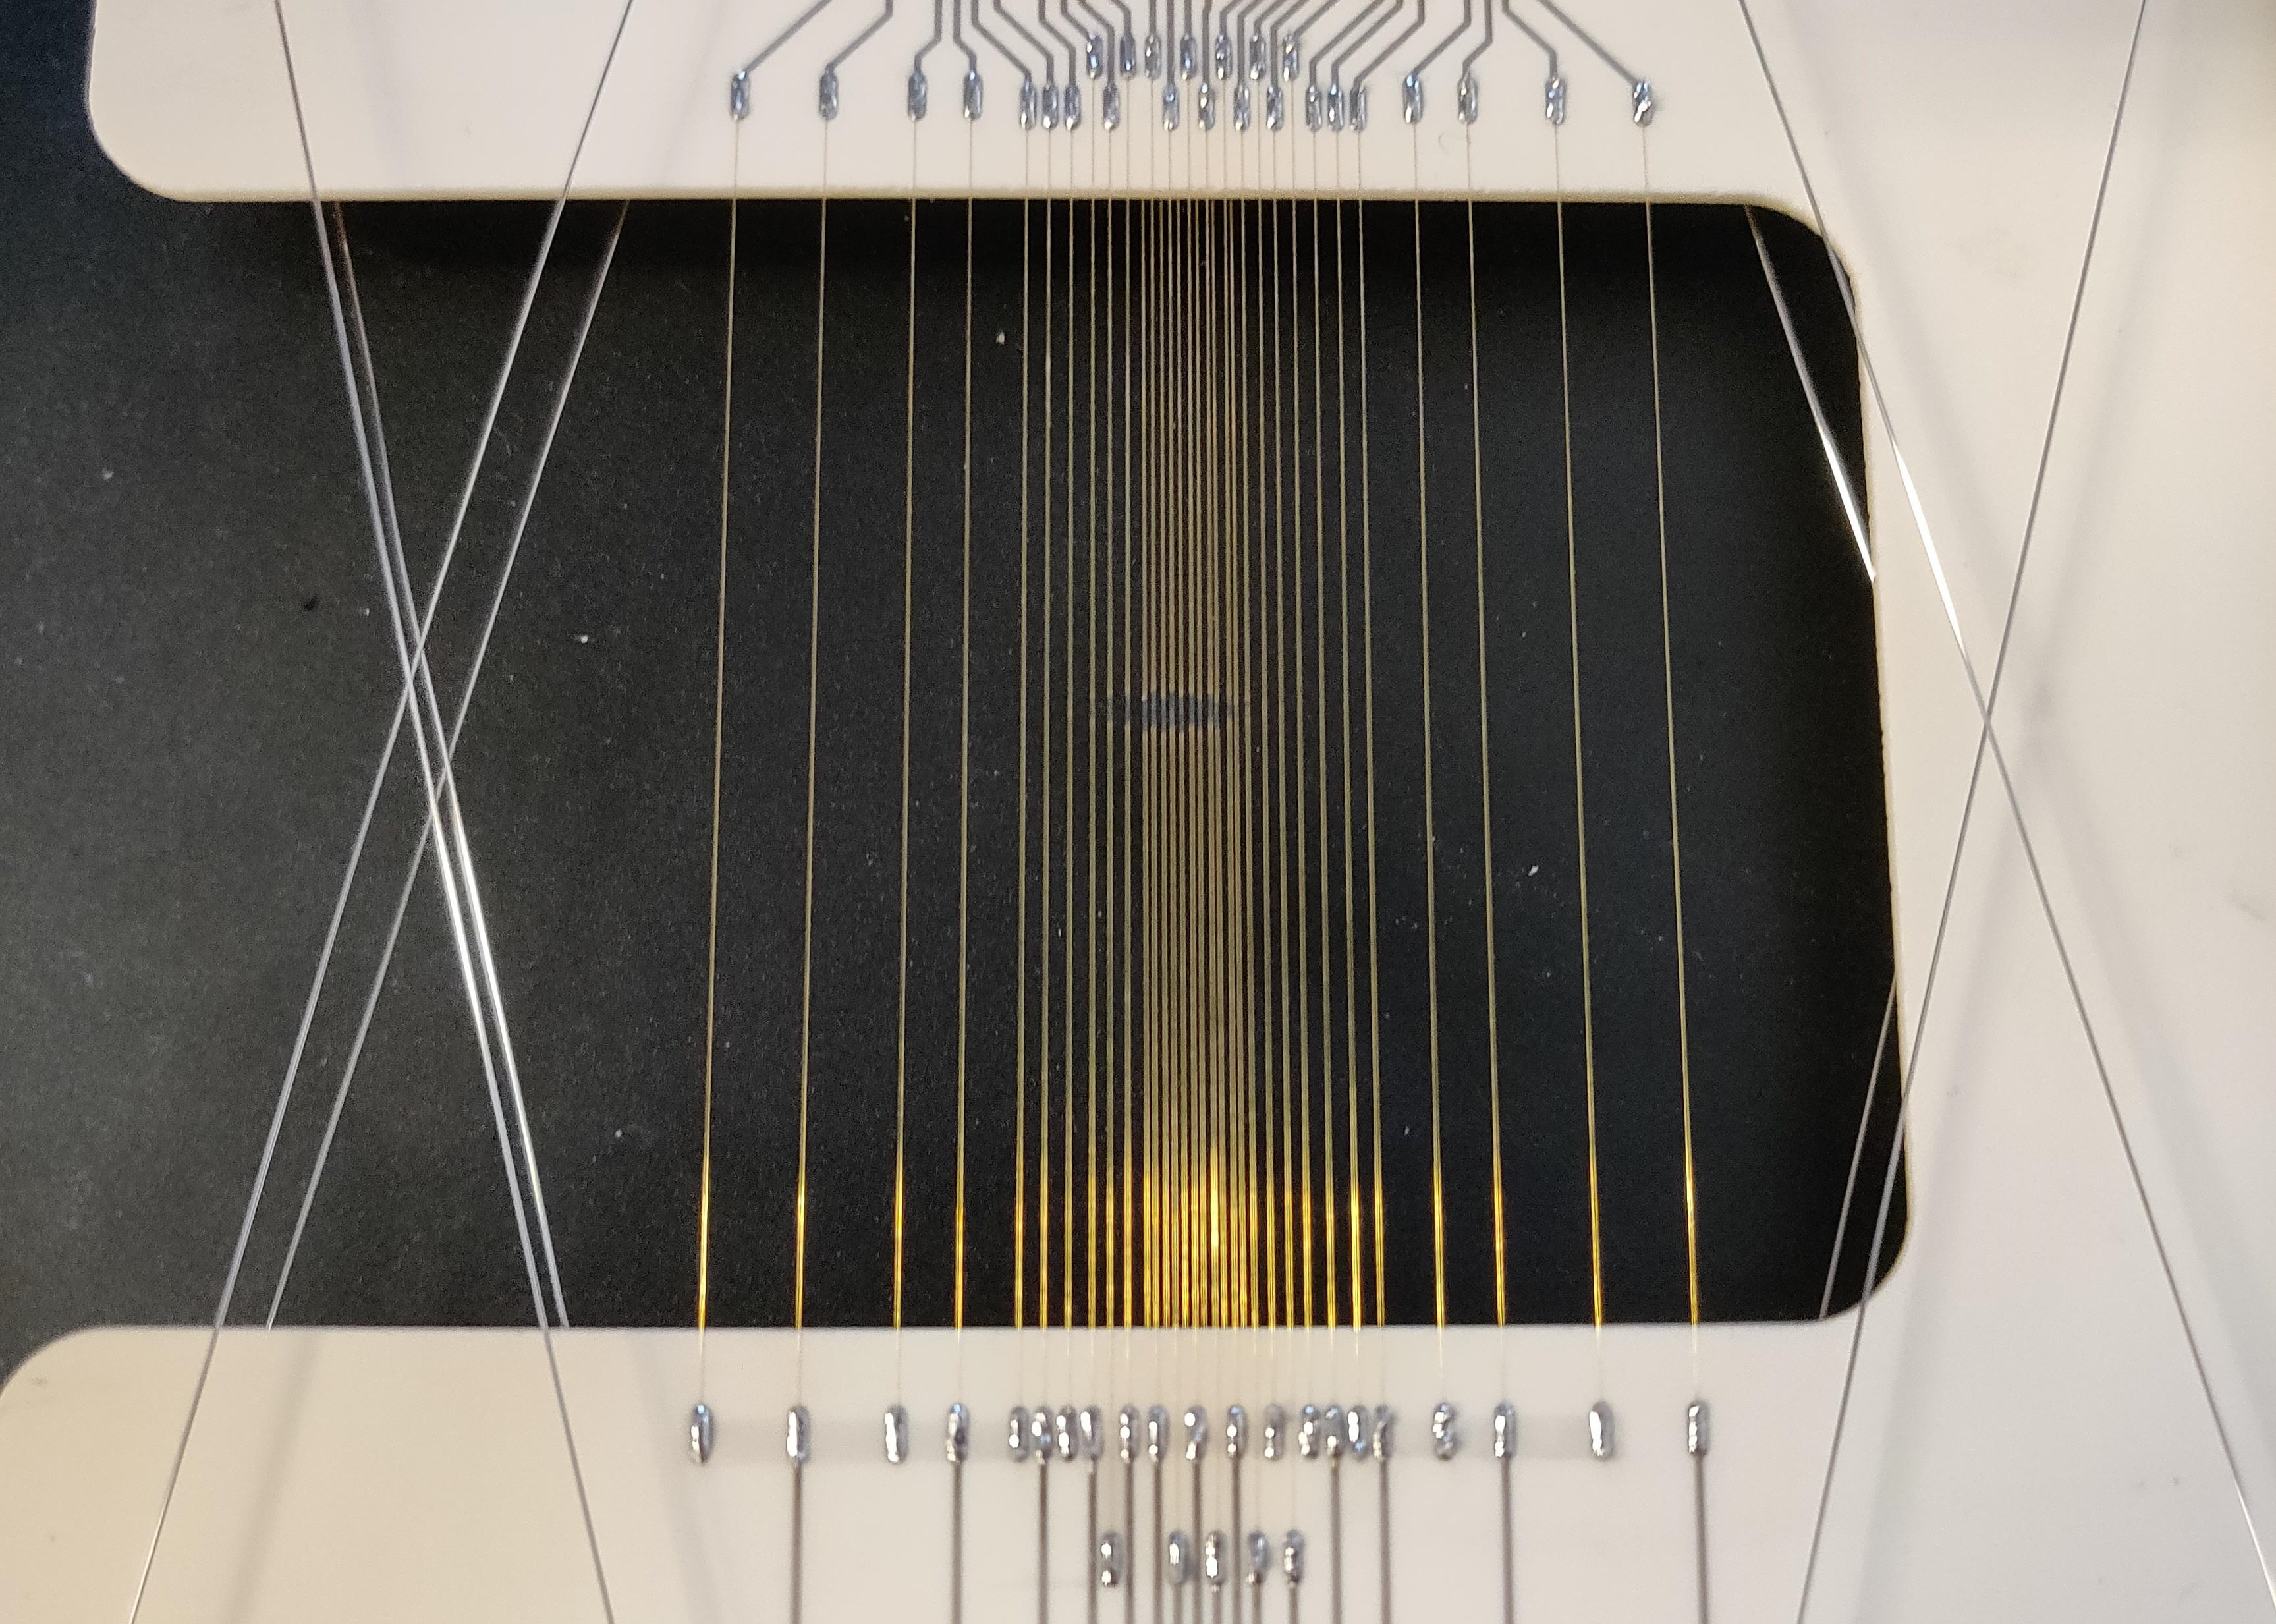
\includegraphics[width=\textwidth]{SEMgridDamage/GridDamage1.jpg}
    \end{subfigure}
    \hspace{0.5cm}
    \begin{subfigure}[b]{0.4\textwidth}
        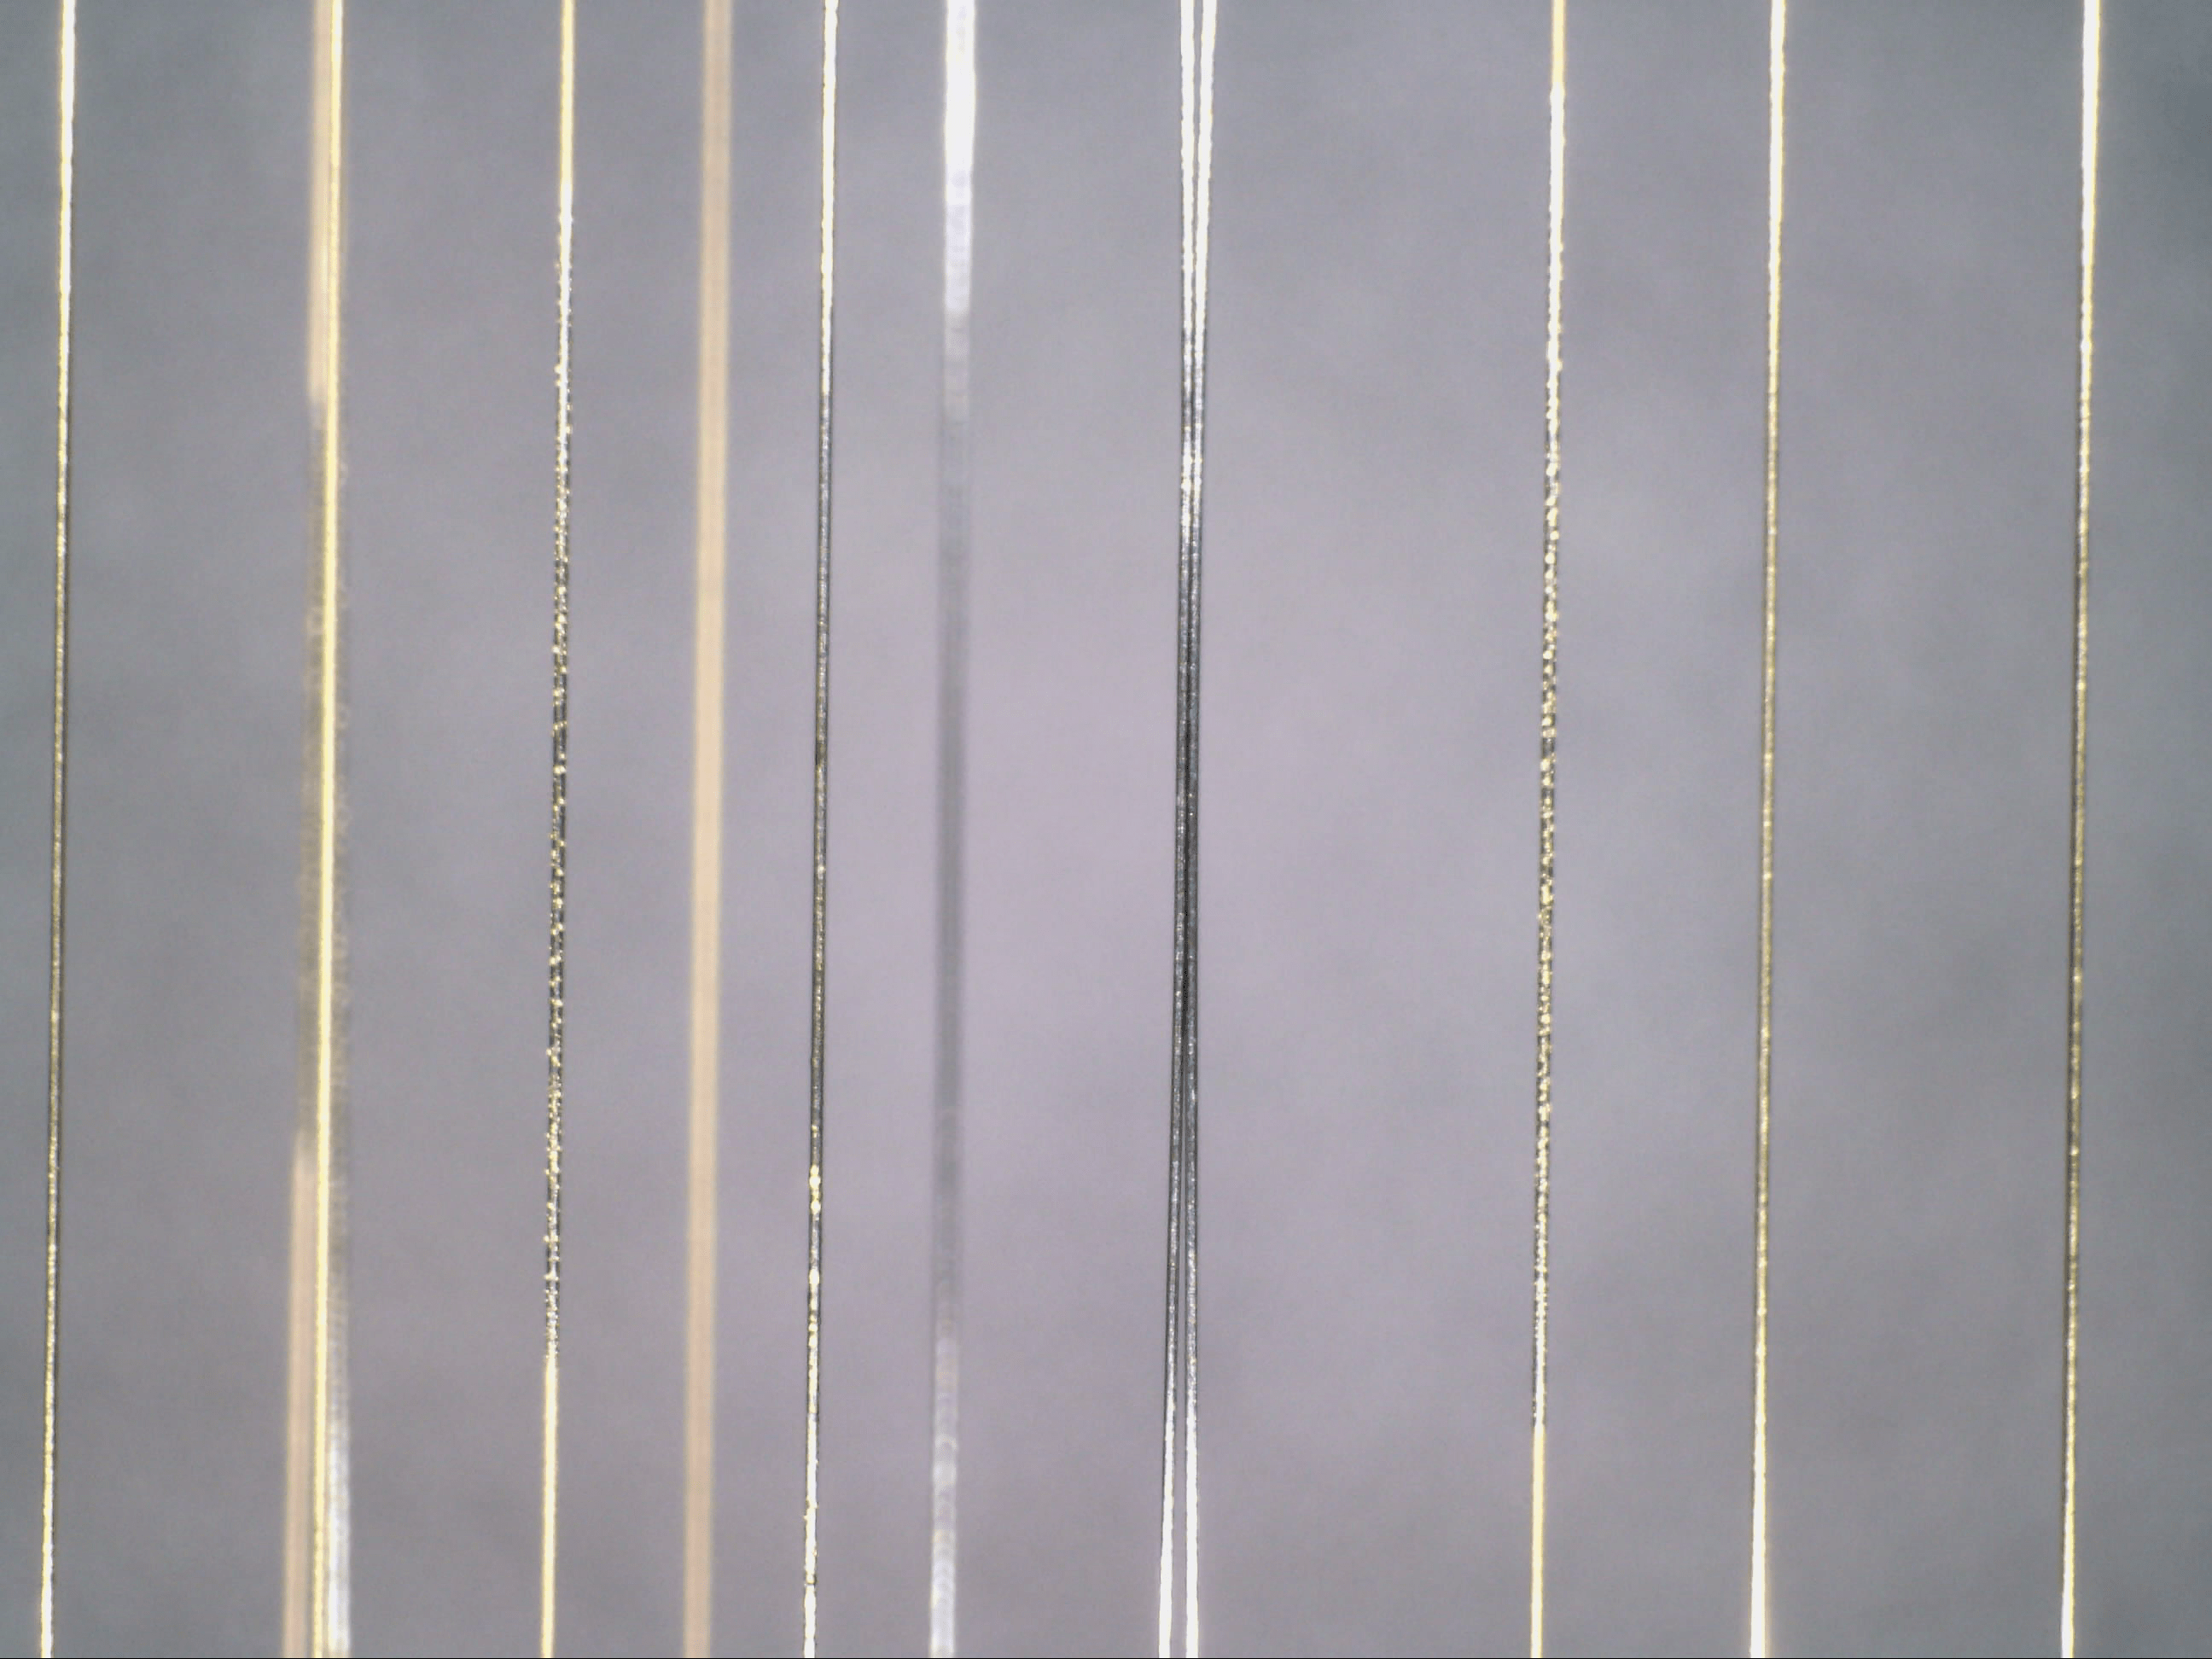
\includegraphics[width=\textwidth]{SEMgridDamage/GridDamage2.png}
    \end{subfigure}
    \caption{SEM Grid used at Linac4, in L4T Line.  }
    \label{fig:SEMLinac4damage}
\end{figure}

Figure \ref{fig:WireGluing} shows the effects wire gluing has on transverse beam profile measurements. These measurements were taken at LINAC4. In this figure, the same transverse beam profile before and after the detector damage is shown. To avoid these permanent damages, a deep understanding of the thermal evolution suffered by the detectors is necessary. 

\begin{figure}[h]
    \centering
    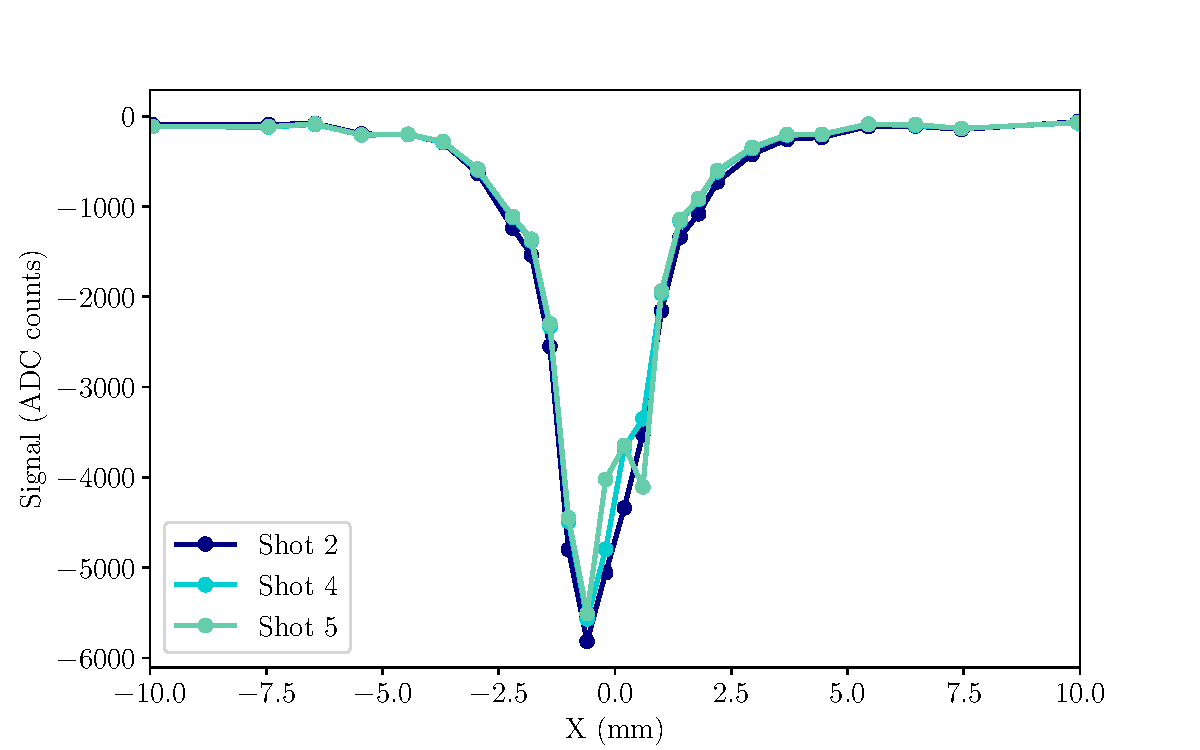
\includegraphics[width=0.60\columnwidth]{Figure_WiresGluing/WireProfile.pdf}
    \caption{Horizontal transverse beam profile of 160 MeV beam of particles at Linac4. Same beam conditions, before and after beam damage. }
    \label{fig:WireGluing}
\end{figure}



\section{The heat equation}

To understand the temperature variation of thin target detectors during operation, we need first to introduce the different processes that collaborate in this thermal evolution. In our case, the temperature variation can be described as: 

\begin{equation}
    \left(\frac{\partial T}{\partial t}\right)_{tot} = \left(\frac{\partial T}{\partial t}\right)_{Ht} - \left(\frac{\partial T}{\partial t}\right)_{Rd} - 
                 \left(\frac{\partial T}{\partial t}\right)_{Cd} - \left(\frac{\partial T}{\partial t}\right)_{Th} - \left(\frac{\partial T}{\partial t}\right)_{Sub}
    \label{eq:HeatBalance}
\end{equation}

Where the term with sub-index Ht represents the beam heating, and it is accompanied by several cooling processes such as radiative cooling (Rd), conduction cooling (Con), thermionic cooling (Th) and sublimation cooling (Sub). Because in our case this thermal model is going to be used for applications in ultra-high vacuum conditions ($10^{-6} - 10^{-9}$ (mbar)), cooling phenomena such as convection are not considered. 

To simplify the notation, the dependences of the different terms have not been included in equation \ref{eq:HeatBalance}. The temperature depends on the time (t) and on the spatial coordinates (x,y). Due to the thin target nature of the detectors, the coordinate (z) along the beam axis will not be considered. 

\subsection{Target Heating (Ht)}

Beam-induced detector heating can be traced down to two possible phenomena: 

\begin{itemize}
    \item Direct Beam Energy Deposition: It is related to nuclear and atomic interactions of the beam of particles with the material of the detector. 
    \item Indirect Electromagnetic Coupling: This is related to the energy exchange due to electromagnetic coupling between the beam of particles and the detector. 
\end{itemize}

Indirect electromagnetic coupling is a phenomenon that can be heavily mitigated by properly designing the detector geometry, and will not be covered in this work. If it is of the reader interest, a detailed description of this phenomenon can be found in \parencite[][]{ref:ElectroHeating}. One can describe the temperature variation due to direct energy deposition as follows: 

\begin{equation}
    \left(\frac{\partial T}{\partial t}\right)_{Ht} = \frac{N (x,y,t)}{V\cdot Cp(T)\cdot \rho (T)}\cdot \frac{dE}{dx}
\end{equation}

Where V, Cp(T) and $\rho (T)$ are the volume, specific heat and density of the detector's material. $dE/dx$ is the single particle energy deposition, which was explained in Chapter \ref{ch:BeamMatterInter}. N(x,y,t) refers to the surface density of beam particles reaching a point in space (x,y) at time t. This concept can be generalized to any particle distribution. However, in most cases, the beam of particles can be described as a Gaussian distribution. In that case, N(x,y) can be described as: 

\begin{equation}
    N(x,y) = \frac{N_{Tot}}{2 \pi \sigma_x \sigma_y}\cdot exp \left(
              -\frac{1}{2}\left(\frac{x-x_0}{\sigma_x}\right)^2 - \frac{1}{2}\left(\frac{y - y_0}{\sigma_y}\right)^2\right)
\end{equation}

Here $x_0$ and $y_0$ represent the coordinates of the beam centroid and $\sigma_x$ and $\sigma_y$ represent the standard deviation of the normally distributed beam of particles. $N_{tot}$ is the total number of particles (per unit time) in the particle beam. The temporal distribution can be approximated as a pulse train function. This means: 

\begin{equation}
    \begin{cases}
      N(x,y,t) = N(x,y) \mspace{30mu} if\mspace{18mu}Beam = Yes \\
      N(x,y,t) = 0 \mspace{80mu} if \mspace{18mu}Beam = No 
    \end{cases}
\end{equation}

\subsection{Radiative Cooling (Rd)}

Radiative cooling occurs due to heat transfer by thermal radiation carried by electromagnetic waves \parencite[][]{ref:RadiativeCooling}. Accelerating charged particles (electrons and protons) in the solid emit photons (or electromagnetic waves) that carry energy with them. In vacuum,  or in materials that allow the transmission of electromagnetic waves, radiation cooling might be of great importance. 

Radiative cooling is a surface effect, and it depends on the surface characteristics and its temperature.  The net temperature variation from a surface S at a temperature T to a surrounding large enclosure at temperature $T_0$ can be described by Stephan-Boltzman's law as follows: 

\begin{equation}
    \left( \frac{\partial T}{dt} \right)_{Rad} = \frac{S\cdot \sigma_{SB}\cdot \epsilon(T)\cdot \left(T(x,y,t)^4 - T_0^4\right)}{Cp(T)\cdot V \cdot \rho(T)}
\end{equation}

Where $\sigma_{Sb}$ is the Stephan-Boltzmann constant and $\epsilon$ is the emissivity of the material. Emissivity is a measure of the efficiency with which a surface emits thermal energy and it is defined as the ratio of the energy radiated from a material's surface to that radiated from a perfect emitter, known as black-body. A more detailed description of the emissivity can be found in chapter \ref{ch:EmissivityMeas}. 

\subsection{Conduction Cooling (Cd)}

Thermal conduction in solids or static fluids \parencite[][]{ref:ConductionCooling} occurs as soon as a spatial temperature gradient exists. The carriers of the energy transfer can be molecules, atoms, electrons and phonons. The rate of change due to conduction can be described by Fourier's equation as follows: 

\begin{equation}
    \left( \frac{\partial T}{\partial t} \right)_{Cond} = \alpha (T) \left( \frac{\partial^2 T}{\partial x^2} + \frac{\partial^2 T}{\partial y^2} \right)
\end{equation}

$\alpha(T)$ is called the thermal diffusivity of the medium and it measures the rate of heat transfer in a material from the hot end to the cold end. It has SI units of $m^2 /s$. It can be calculated as follows: 

\begin{equation}
    \alpha(T) = \frac{k(T)}{\rho(T)Cp(T)}
\end{equation}

Where k(T) is defined as the thermal conductivity of the material (W/mK), which is the measure of the capability of the material to conduct heat. In general, metals have high thermal conductivity and gases have low thermal conductivity. 

\subsection{Thermionic Cooling (Th)}

Thermionic emission was introduced in chapter \ref{ch:CurrentModeling}. As was said before, thermionic emission is a process by which free electrons are emitted from the surface of a metal when they gain enough thermal energy to overcome the work function. These thermionic electrons take with them some energy, and this contributes to the thermal cooling \parencite[][]{ref:ThermoCooling}. The temperature variation due to thermionic emission can be described as: 

\begin{equation}
    \left(\frac{\partial T}{\partial t}\right)_{Th} = S\cdot \left( \phi +2K_B T\right)\cdot \frac{J_{Th}(T)}{C_p(T)\cdot V \cdot \rho(T)}
\end{equation}

Where $\phi$ is the work function of the material. $K_B$ is Boltzmann constant. $J_{th} (T)$ was described in section \ref{sec:ThermoCurrent} can be written as: 

\begin{equation}
    J_{th} (T) = A_R \cdot T^2\cdot exp\left(-\frac{\phi}{K_B T}\right)
\end{equation}

\subsection{Sublimation Cooling (Sub)}

Sublimation is the process of changing a solid into a gas without passing through the liquid phase. To sublimate a substance, certain energy must be provided. We will call this energy $H_{sub}$, and it must be sufficient to break the intermolecular forces holding the solid together. Usually it is expressed in (KJ/mol) and can be found in the literature. Similar to the thermionic case, the newly formed gas molecules will escape the material, and the energy given to them for transforming their estate contributes to the overall cooling of the detector \parencite[][]{ref:SublimationCooling}. This sublimation cooling can be written as: 

\begin{equation}
    \left(\frac{\partial T}{\partial t}\right)_{Sub} = H_{sub}\cdot n(T)
\end{equation}

n(T) is the material sublimation rate. Following the same procedure as \parencite[][]{ref:SubRate}, one can determine an upper limit of this sublimation rate. For that one needs to assume the following: 

\begin{itemize}
    \item No atoms leaving the boundary layer return to the hot surface. 
    \item A thin boundary layer over the hot material surface is at equilibrium with the substance sublimation pressure ($P_{vap}$) for temperature $T_{vap}$. 
    \item This thin layer of gas is considered to be an ideal gas. 
\end{itemize}

With these approximations, the amount of sublimated material per unit of time can be expressed as: 

\begin{equation}
    d_{sub} = \frac{1}{2}v_{vap}\cdot \rho_{vap} \cdot \rho_{c}
    \label{eq:SubMaterial}
\end{equation}

$v_{vap}$ is the velocity of the vapor particles. From an ideal gas theory, we know that the average velocity of gas particles in a hemisphere can be described as follows: 

\begin{equation}
    v_{vap} = \frac{1}{2}\cdot \sqrt{\frac{8k_B T_{vap}}{m \pi}}
\end{equation}

Where m is the mass of the material particle. In equation \ref{eq:SubMaterial}, $\rho_{vap}$ refers to the vapor density in the equilibrium layer and can be expressed using the formula: 

\begin{equation}
    rho_{vap} = \frac{m_{mol} T_{std}}{V_{mol} P_{atm}}\cdot \frac{P_{vap}(T_{vap})}{T_{vap}}
\end{equation}

Where $P_{atm}$ is the atmospheric pressure ($10^5$ Pa), $V_{mol} = 22.4$ $dm^3$is the molar volume of an ideal gas at the standard temperature $T_{std} = 273$ K. The vapor pressure highly depends on the maximum temperature of the material, and thus, the total amount of sublimated material will highly depend on the temperatures reached. 

\section{Numerical Approximation to the heat equation.}

Putting together all the concepts from the previous section, we can re-write equation \ref{eq:HeatBalance} as follows: 

\begin{multline}
    \left(\frac{\partial T}{\partial t}\right)_{Tot} = 
    \frac{N(x,y,t)}{V\cdot Cp(T) \cdot \rho (T) }\cdot \frac{dE}{dx} \\
    - \frac{S\cdot \sigma_{SB}\cdot \epsilon(T)\cdot \left(T^4 - T_0^4\right)}{Cp(T)\cdot V \cdot \rho(T)} 
        -\alpha (T) \left( \frac{\partial^2 T}{\partial x^2} + \frac{\partial^2 T}{\partial y^2} \right)  \\
        - S\cdot \left( \phi +2K_B T\right)\cdot \frac{J_{Th}(T)}{C_p(T)\cdot V \cdot \rho(T)} - H_{sub} \cdot n(T)
    \label{eq:ExplicitHeatEq}
\end{multline}

This is an evolutionary, non-linear, second order, partial differential equation (PDE). In this work, this equation is treated numerically. The subject of PDEs and how to solve them is very broad. An enormous number of different numerical techniques to solve non-linear or quasi-linear PDEs exist. For an outstanding introduction to this world, I recommend the reader to check \parencite[][]{ref:NumericalMethodBook}, where a small number of tools are introduced forming a solid basis for the understanding of the subject. 

In this document, we will focus on the classical theory of finite differences. The main idea in the calculus of finite differences is to replace derivatives with linear combinations of discrete function values. The word discrete means that the numerical solution is known only at a finite number of points (or nodes) in the physical domain. Figure \ref{fig:SpaceDiscret} shows an example of the spatial discretization of a homogeneous body. 

\begin{figure}[h]
    \centering
    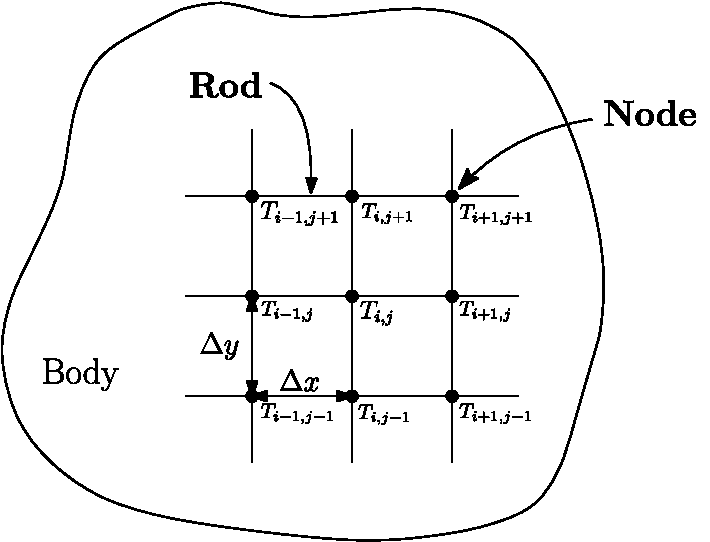
\includegraphics[width=0.5\columnwidth]{SpaceDiscretization/SpaceDiscretization.pdf}
    \caption{Space discretization of a homogeneous body.}
    \label{fig:SpaceDiscret}
\end{figure}

The parameters $\Delta x$ and $\Delta y$ indicate the local distance between adjacent points in space, and in our case, they are considered to be uniform throughout the mesh. Increasing the number of nodes in the mesh (reducing $\Delta x , \Delta y$) increases the resolution and the accuracy of the numerical solution. However, it increases computational costs.

Every node in the grid has a temperature and can exchange heat with its neighbors through a heat conducting rod. The sub-indexes i, j are used to refer to nodes in the physical space.  $T_{i,j}$ refers to the temperature in the position $x_i , y_j$.

Because the temperature of the system changes a function of time, the numerical solution of the PDE requires also time discretization. Figure \ref{fig:TimeDiscret} shows a schematic representation of the time discretization of a strip of material. The time nodes are referred to with the super-index m, so that $T^{m}$ corresponds to the temperature at the time instant  $t^m$.  $\Delta t$ refers to the difference between time nodes. This distance was also considered to be equidistant, however, two different time constants were considered, one for the heating time ($\Delta {t}_{heat}$) and one for the cooling period ($\Delta t_{Coold}$). In most applications, the beam of particles is pulsed, and the beam pulse length is much shorter than the period without beam. 

\begin{figure}[h]
    \centering
    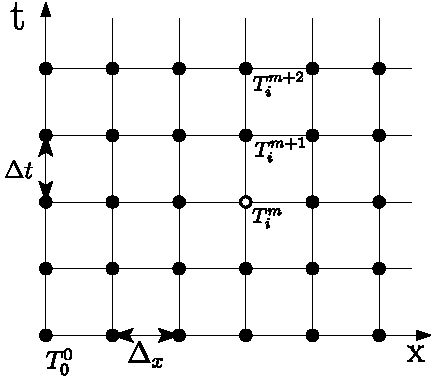
\includegraphics[width=0.4\columnwidth]{TimeDiscretization/TimeDiscret.pdf}
    \caption{Time discretization of the material rod.}
    \label{fig:TimeDiscret}
\end{figure}

\section{Finite Differences Schemes}
\label{sec:FD}

Working with the full heat equation (eq. \ref{eq:ExplicitHeatEq}) can result in a very cumbersome notation. 
The one-dimensional case of a thin rod will be considered, with only radiative and conduction cooling will be considered in this section. The concepts can be easily extrapolated to the full 2D case and some hints on that will be given in the following sections.  The simplified equation that we will treat here is: 

\begin{equation}
    \frac{\partial T(x,t)}{\partial t} = 
        H(x,t,T)
        - A(T) \left(T(x,y)^4 - T_0^4\right)
            -\alpha (T)  \frac{\partial^2 T(x,t)}{\partial x^2}   
            \label{eq:SimpleHeating}
    \end{equation}

Where H(x,t) refers to the heating term. A(T) can be written as: 

\begin{equation}
    A(T) = \frac{S\cdot \sigma_{SB}\cdot \epsilon(T)}{Cp(T)\cdot V \cdot \rho(T)}. 
\end{equation}

At any instant of time, one has access only to the values of the temperature at the afore-mentioned nodes ($T^{m}_{ij}$). The objective now is to obtain an approximation of $\partial T/dt$, $\partial^2 T,\partial x^2$ and $\partial^2 T/\partial y^2$ in those nodes by only knowing the information provided by the other nodes. Using different combinations of the mesh points results in different schemes. In the following, three of these schemes will be introduced. For a more detailed description of these methods, one can check the reference \parencite[][]{ref:FiniteDifference}.

\subsection{Forward in Time, Centered in Space (FTCS)}

This scheme approximates the time derivative with a forward difference: 

\begin{equation}
    \left. \frac{\partial T}{\partial t}\right|_{t^{m+1},x_i}  = \frac{T^{m+1}_i - T^m_i}{\Delta t} +  \mathcal{O} \left( \Delta t \right)
 \end{equation}

And for $\partial^2 T/ \partial x^2$ a central difference approximation is used. 

\begin{equation}
    \left. \frac{\partial^2 T}{\partial x^2}\right|_{x_i} = \frac{T^{m}_{i-1}-2T^m_{i}+T^m_{i+1}}{\Delta x^2}+\mathcal{O}\left(\Delta x^2 \right)
    \label{eq:CD}
\end{equation}

The expression $\mathcal{O}(\Delta t)$ is telling us, that the local truncation error, in this case, is proportional to the time step size, while $\mathcal{O}(\Delta x)$ indicates that the truncation error reduces quadratically with the spatial step size. 

\begin{figure}[h]
    \centering
    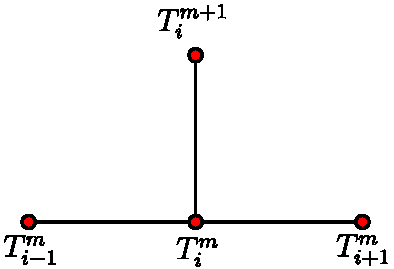
\includegraphics[width=0.35\columnwidth]{Stencils_FiniteDifferences/FTCS.pdf}
    \caption{Stencil for the Forward Time, Central Space finite difference method.}
    \label{fig:StencilFTCS}
\end{figure}

The stencil of this method can be found in figure \ref{fig:StencilFTCS}. This is considered an explicit method, as it calculates the state of the system at a later time from the state of the system at the current time. 

Introducing these approximations in equation \ref{eq:SimpleHeating}:

\begin{equation}
    \frac{T^{m+1}_i - T^m_i}{\Delta t} = H^m_i - A_i^m \left((T_i^m )^4 - (T_0)^4\right) +\alpha_i^m    \frac{T^{m}_{i-1}-2T^m_{i}+T^m_{i+1}}{\Delta x^2}
\end{equation}

After a little bit of algebra, this equation can be written in a matrix form.

$$
\begin{bmatrix}
         1 & 0 & 0 & 0 & 0 & 0 \\
         r^m_1 & \left(1-2r^m_1\right) & r^m_1 & 0 & 0 & 0 \\ 
         0 & r & \left(1-2r^m_1\right) & r^m_1 & 0 & 0 \\ 
         0 & 0 & \ddots & \ddots & \ddots & 0 \\
         0 & 0 & 0 & r^m_1 & \left(1-2r^m_1\right) & r^m_1 \\
         0 & 0 & 0 & 0 & 0 & 1 
     \end{bmatrix}
\begin{bmatrix}
         T^m_0  \\
         T^m_1 \\ 
         T^m_2  \\ 
         \vdots \\
         T^m_{N-1} \\
         T^m_N 
     \end{bmatrix}
     =
     \begin{bmatrix}
         T^{m+1}_0 + g(T^m_0) \\
         T^{m+1}_1 + g(T^m_1)\\ 
         T^{m+1}_2 + g(T^m_2)\\ 
         \vdots\\ 
         T^{m+1}_{N-1} + g(T^m_{N-1})\\
         T^{m+1}_{N} + g(T^m_{N}) 
     \end{bmatrix}
$$

With $r^m_i = \alpha^m_i \cdot \Delta t/ \Delta x^2$. And with g(T) including all the non-linear terms of the equation. In a more simplified way: 

\begin{equation}
    D_{FTCS}\cdot T^{m} = T^{m+1}+g(T^m)
\end{equation}

This is a relatively simple method to implement, as the values of $T_i^{m+1}$ can be updated independently of each other. However, the FTCS method can yield unstable solutions that can oscillate and grow if $\Delta t$ is too large. A stable solution with FTCS scheme is only obtained if: 

\begin{equation}
    r = \alpha\cdot \frac{\Delta t}{\Delta x} < \frac{1}{2}
    \label{eq:rstab}
\end{equation}

See \parencite[][]{ref:proveR1} and \parencite[][]{ref:proveR2} for a proof that equation \ref{eq:rstab} gives the stability condition for FTCS. 

\subsection{Backwards in Time, Centered Space (BTCS)}

In this case, a backward in time difference is used to approximate the time derivative while a central space scheme is used for the spatial derivative: 

\begin{equation}
    \left. \frac{\partial T}{\partial t} \right|_{t^{m+1},x_i} = \frac{T^m_i - T^{m-1}_i}{\Delta t}+\mathcal{O}(\Delta t)
\end{equation}

As in the previous case, the full equation can be represented in a matrix form: 

$$
\begin{bmatrix}
         b_0 & c_0 & 0 & 0 & 0 & 0 \\
         a_1 & b_1 & c_1 & 0 & 0 & 0 \\ 
         0 & a_2 & b_2 & c_2 & 0 \\ 
         0 & 0 & \ddots & \ddots & \ddots & 0 \\
         0 & 0 & 0 & a_{N-1} & b_{N-1} & c_{N-1} \\
         0 & 0 & 0 & 0 & a_N & b_N 
     \end{bmatrix}
\begin{bmatrix}
         T^m_0  \\
         T^m_1 \\ 
         T^m_2  \\ 
         \vdots \\
         T^m_{N-1} \\
         T^m_N 
     \end{bmatrix}
     =
     \begin{bmatrix}
         d_0 + g(T^m_0) \\
         d_1 + g(T^m_1)\\ 
         d_2 + g(T^m_2)\\ 
         \vdots\\ 
         d_{N-1} + g(T^m_{N-1})\\
         d_{N} + g(T^m_{N}) 
     \end{bmatrix}
$$

Where the coefficients are:

\begin{equation}
    \begin{gathered}
        a_i = -r^m_{i-1} \\
    b_i = 1 + 2r^m_{i}\\
    c_i = - r^m_{i+1} \\
    d_i = T^{m-1}_i + g(T_i^m)
    \end{gathered}
\end{equation}

Figure \ref{fig:StensilBTCS} shows the stencil representation of this method. In this case, we are dealing with an implicit method. To find the temperature in the time step m one must solve an equation involving both the current state of the system (m) and the previous state (m-1). 

\begin{figure}[h]
    \centering
    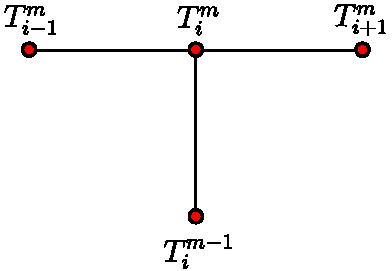
\includegraphics[width=0.35\columnwidth]{Stencils_FiniteDifferences/BTCS.pdf}
    \caption{Stencil for the Backwards in time, Central in space finite difference method.}
    \label{fig:StensilBTCS}
\end{figure}

\subsection{Crank-Nicolson}

To improve the temporal truncation error, the Crank-Nicolson scheme approximates the spatial derivative by the average of the central difference scheme, evaluated in the current (m) and the previous (m-1) time steps: 

\begin{equation}
    \frac{T^m_i - T^m_i}{\Delta t} = g(T^m_i) + \frac{\alpha^m_i}{2}\left[ 
          \frac{T^m_{i-1}- 2 T^m_i + T_{i+1}^m}{\Delta x^2} + \frac{T^{m-1}_{i-1}-2T^{m-1}_i+T_{i+1}^{m-1}}{\Delta x^2}
    \right] 
\end{equation}

This method is implicit, like the BTCS method. However, it accomplishes a truncation error $\mathcal{O}(\Delta t^2)$ without overcomplicating the implementation. The matrix representation is the same as in the BTCS case, but with the following coefficients:

\begin{equation}
    \begin{gathered}
        a_i = -r^m_{i-1}/2 \\
        b_i = 1 + r^m_{i}\\
        c_i = - r^m_{i+1}/2 \\
        d_i = a_i T_{i-1}^{m-1} + (1 + a_i + c_i) T^{m-1}_{i} + c_i T_{i+1}^{m-1} + g(T_i^m)
    \end{gathered}
\end{equation}

The stencils representation of this method is shown in Figure \ref{fig:StencilCrNic}.

\begin{figure}[h]
    \centering
    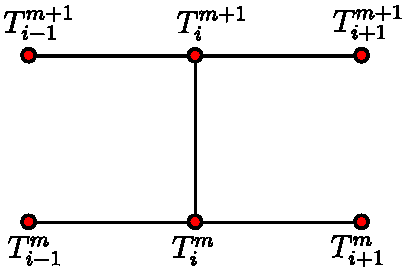
\includegraphics[width=0.35\columnwidth]{Stencils_FiniteDifferences/CrkNic.pdf}
    \caption{Stencil for the Crank-Nicolson finite difference method.}
    \label{fig:StencilCrNic}
\end{figure}

\section{Initial and Boundary Conditions}

Due to the time dependent part of our equation, we need an initial condition. In this case, this refers to the temperature of the system at time $t^0$. Unless specified otherwise, a constant temperature $T_{i,j}^0 = 300 (K)$ will be considered.

At each time step, because of the spatial dependence of the equation, some boundary conditions need to be specified. Here the so-called Dirichlet boundary conditions are considered. For the one-dimensional case, these conditions can be written as follows: 

\begin{equation}
    \begin{cases}
      T(0,t) = 300 \mspace{30mu} (K) \\
      T(L,t) = 300 \mspace{30mu} (K) 
    \end{cases}
\end{equation}

Where L refers to the length of the one-dimensional rod. In the 2D case, these conditions would indicate that all the borders of the foil are in contact with a thermal sink at 300 (K). 

\section{The Non-Linear Problem}

In the previous sections, g(T) was described as the non-linear term. The explicit expression is: 

\begin{equation}
    g(T) = \frac{N(x,t)}{V\cdot Cp(T)\cdot \rho(T)}\frac{dE}{dz} - \frac{S\cdot \sigma_{SB}\epsilon(T)\cdot \left( T(x,t)^4 - T_0^4\right)}{V\cdot Cp(T)\cdot \rho(T)}
\end{equation}

In the case with no heating and no radiative cooling, g(T) = 0. This case yields to the diffusion equation. In this scenario, the systems of equations presented in the previous section can be easily solved by techniques such as Gaussian elimination methods, LU factorization, etc. More information about those methods can be found in \parencite[][]{ref:AlvaroBook}. 

$g(T) \neq 0$ implies that now, at each time stem, one has to solve a system of non-linear equations. This is still solvable numerically, but it implies using other numerical techniques such as Newton's method for non-linear systems \parencite[][]{ref:AlvaroBook}. At every time step, one must guess an approximate solution and compute the Jacobian matrix. Which can be computationally expensive and cumbersome. 

By default, instead of considering the full equation, each term of the equation is considered separately and then added together. For equation \ref{eq:SimpleHeating} this would mean solving the following: 

\begin{equation}
    \frac{\partial \Delta T_{Ht} (x,t)}{\partial t} = H(x,t,T)
\end{equation}
\begin{equation}
    \frac{\partial \Delta T_{Rad} (x,t)}{\partial t} = A(T) \left(T(x,y)^4 - T_0^4\right)
\end{equation}
\begin{equation}
    \frac{\partial \Delta T_{Con}}{\partial t} = \alpha(T)\frac{\partial^2 T(x,t)}{\partial x^2}
\end{equation}

The total temperature variation is then calculated as: 

\begin{equation}
    \Delta T_{tot} = \Delta T_{Ht} - \Delta T_{Rd} - \Delta T_{Con}
\end{equation}


\section{The two-dimensional problem}

In the previous section, we developed the equations for the one-dimensional case due to the simpler notation. The biggest difference in the two-dimensional case is the conduction term on the heat equation. Each point in space is now connected to four other points, that is, there is conduction along four rods. Figure \ref{fig:1Dvs2D} shows a schematic representation of the differences between nodal connections in a 1D and 2D case.  

\begin{figure}[h]
    \centering
    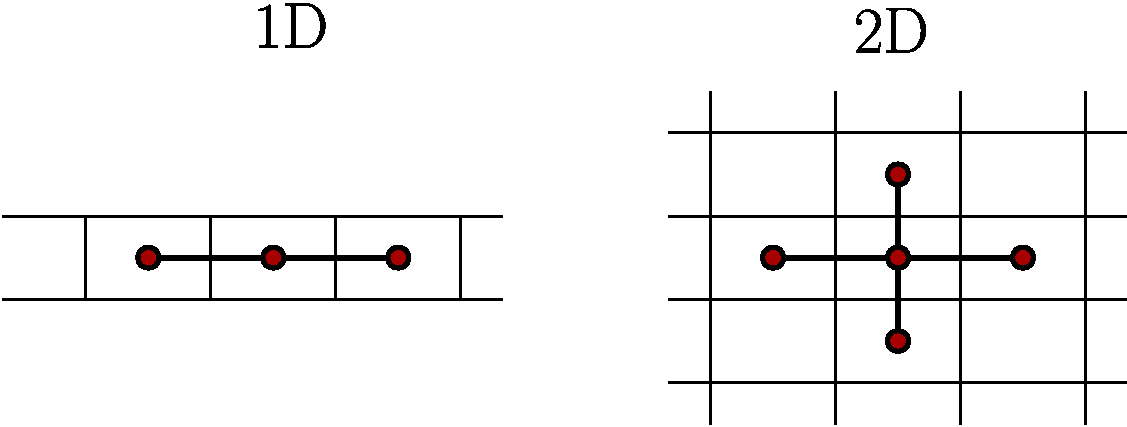
\includegraphics[width=0.60\columnwidth]{1D_vs_2D_cond/1Dvs2F.pdf}
    \caption{Schematical comparison between 1D (left) and 2D (right) nodal connection.}
    \label{fig:1Dvs2D}
\end{figure}

For the two-dimensional case, a five-point finite difference formulation is used \parencite[][]{ref:FiniteDifference}. Taking the simplified case of the 2D diffusion equation: 

\begin{equation}
    \frac{\partial T(t,x,y)}{\partial t} = \alpha (T) \left(\frac{\partial^2 T}{\partial x^2}+\frac{\partial ^2 T}{\partial y^2}\right)
\end{equation}

One could write the FTCS formulation as follows: 

\begin{equation}
    \frac{T_{i,j}^{m+1} - T_{i,j}^{m}}{\Delta t} = \alpha(T_{i,j}^{m}) \left( \frac{T_{i-1,j}^{m} -2T_{i,j}^{m}+T_{i+1,j}^{m}}{\Delta x^2} +  \frac{T_{i,j-1}^{m}-2T_{i,j}^{m}+T_{i,j+1}^{m}}{\Delta y^2} \right)
\end{equation}

Similarly, this could be applied to the BTCS and Crank-Nicolson formulations. The same procedure to transform this into a system of equations can also be followed. 

\section{Importance of Cooling Effects}

The most accurate simulation is obtained when all the cooling mechanisms indicated in equation \ref{eq:HeatBalance} are considered. However, if simulation speed is what matters, a fuster simulation can be run by ignoring certain cooling mechanisms. Particularly, conduction cooling is the most time-consuming one. Figure \ref{fig:CoolingComparison} shows how much each cooling mechanism contributes to the total cooling as a function of the temperature. This figure was calculated for a $30 \mu m$ Graphite wire. It might differ slightly for different materials and geometries. 

From this figure, one can observe how radiation cooling is the predominant mechanism throughout the biggest temperature range. Conduction cooling plays a very important role at lower temperatures while thermionic and sublimation cooling are important only at very high temperatures. 

If there is some a-priory knowledge of the expected temperature range, or simply a fast upper limit of the maximum temperature is needed, various cooling processes can be deliberately eliminated for speed purposes.

\begin{figure}[h]
    \centering
    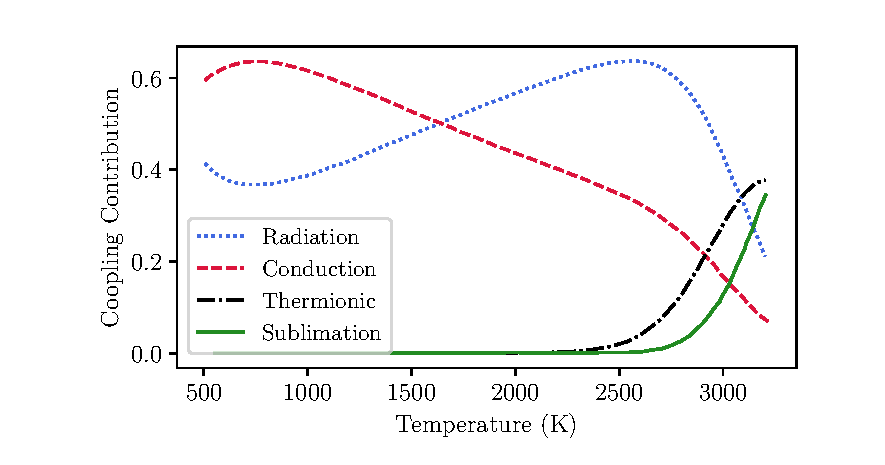
\includegraphics[width=0.60\columnwidth]{PlotCoolingImportancfe/CoolingImpo.pdf}
    \caption{Relative importance of the different cooling mechanisms as a function of the temperature.}
    \label{fig:CoolingComparison}
\end{figure}

\section{PyTT}

The simulation program was implemented using Python 3.6.9. The latest version of the code can be found at \parencite[][]{ref:GitAra}. As aforementioned, the main objective of this code is to quickly obtain an estimation of the maximum temperature reached by thin target detectors when interacting with the beam of particles. Additionally, the code also needed to be easy to use by people who aren't particularly familiar with python or numerical techniques.

Figure \ref{fig:UserFriendly} shows the GUI of the implemented program. The program can also be run directly, without the GUI which allows for easy parallelization. The implementation of the code and its usage will not be discussed in this document. Just the main description of its functionalities will be given. 

\begin{figure}[h]
    \centering
    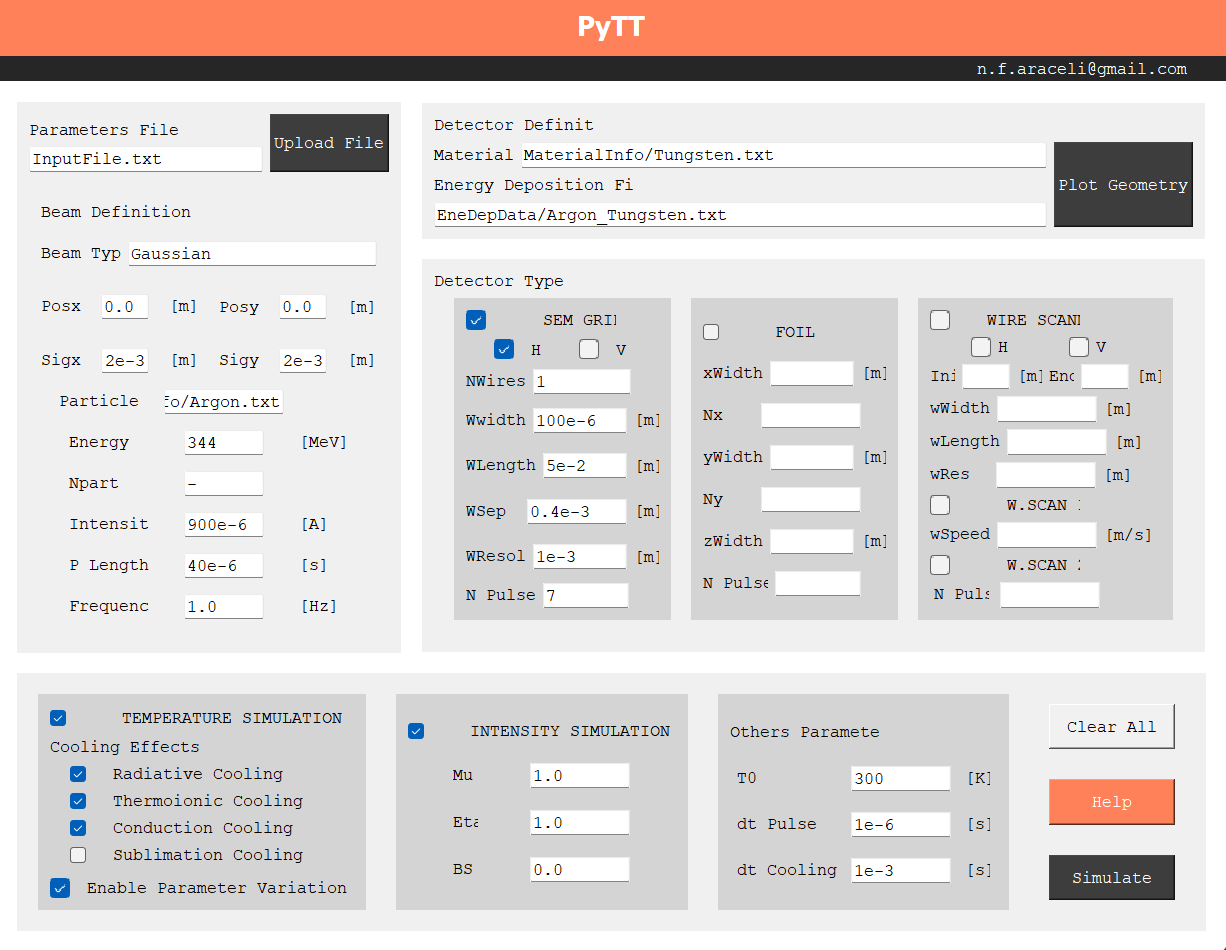
\includegraphics[width=0.9\columnwidth]{PyTT_GUI/PyTTScreanshot.png}
    \caption{Graphical User-Friendly interface of PyTT code.}
    \label{fig:UserFriendly}
\end{figure}

\begin{enumerate}
    \item Variety of Beam Conditions: To simulate a variety of cases, the program allows the user to choose several beam parameters. For example, the particle or ion type and energy, the spatial and temporal distribution, and the repetition frequency of the particle beam. 
    \item Variety of Detector Materials: The material of the detector can be chosen freely, by either selecting one of the already given materials or by easily creating one's own. 
    \item Type of thin target detectors: The program can simulate SEM grid detectors, Thin foils and Wire scanners. For the wire scanners, both fast and slow wire scanners can be considered. 
    \item Choosable simulation Parameters:  Several simulation parameters (Such as space-time discretization parameters, simulation length, thermal effects, parameter temperature dependence, etc.) Can be easily selected at the user's convenience. 
    \item Intensity Simulation: The program includes an intensity simulation module that includes the model explained in chapter \ref{ch:CurrentModeling}. This calculates the current generation in the detector during operation. 
\end{enumerate}

Results like the maximum temperature in the detector as a function of time are provided by default. Figure \ref{fig:GUIResults} shows an example of the simulated output. However, using the output files produced by the simulation, some additional results can be attained. These can include, spatial thermal distributions, the relative importance of the different cooling methods, the evolution of material properties during simulation, intensity distribution, etc. 

\begin{figure}[h]
    \centering
    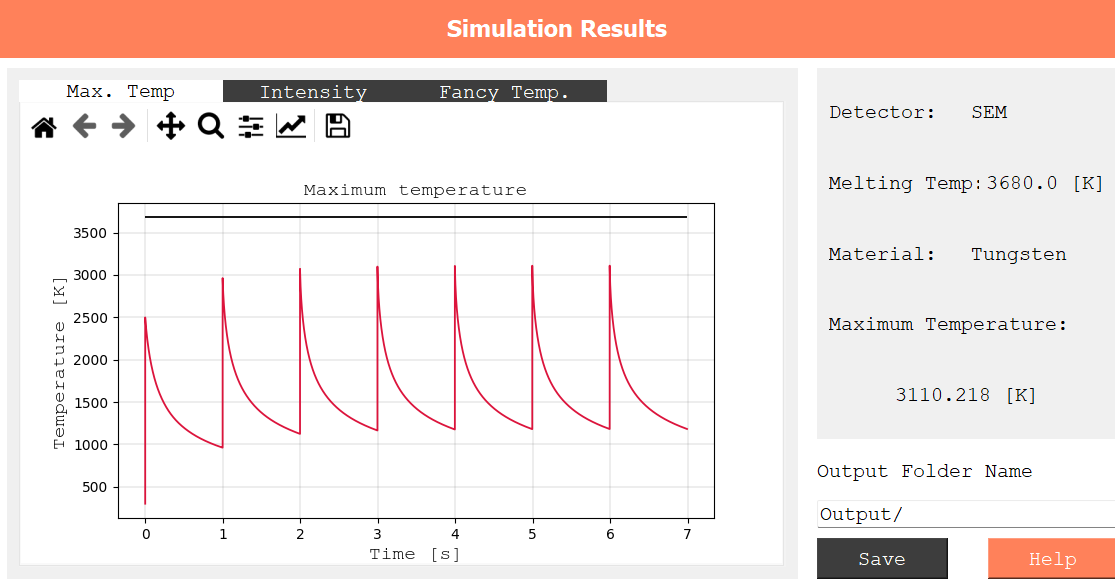
\includegraphics[width=0.9\columnwidth]{PyTT_GUI/PyTTresults.png}
    \caption{Example of output visualization GUI.}
    \label{fig:GUIResults}
\end{figure}

The program has been optimized for it to be used by the python interface. However, it can also be launched by a stand-alone executable for windows systems. A more detailed description of how to use the code can be found in the user manual, accessible through the help button in the GUI, or directly in the HelpFolder.

\section{Model uncertainties}
\label{sec:ModelUnc}

As with all models, the approximations done along the way induce uncertainties in the final results. In section \ref{sec:FD} we talked about the order of truncation errors. We saw how errors were related to the selection of space-time discretization sizes. In this section, we will talk about other sources of error that have proven to be more significant than the numerically induced uncertainties. 

The simulation results highly depend on our knowledge of the simulation case. That is, the better one is able to describe the experimental situation, the more accurate the simulated results. However, a lot of different parameters are involved in this description. To simplify the study one can divide these parameters into two categories: Beam Parameters and Material Properties. 

\subsection{Beam Parameter Uncertainties.}

These parameters are the ones used to describe the spatial and temporal distribution of the beam of particles. If we take as an example the case of a Gaussian beam, those parameters would be: beam size ($\sigma_x , \sigma_y$), beam position, Intensity, pulse length, repetition rate, etc. 

Figure \ref{fig:BeamParUnc} shows how uncertainties in the beam parameters affect the final temperature simulated results. To clarify, to calculate these values, a case was considered to be the average, or correct solution. All the parameters were varied independently up to a $\pm 30\%$ of their value (Parameter Rel. Error)  and the relative error of the simulation was calculated in each case with respect to the average solution. 

From this figure, we can observe that uncertainties in the beam Intensity and pulse length give an almost identical uncertainty response, which increases linearly with the parameter uncertainty. Uncertainties in the beam size, greatly affect the final uncertainties in the maximum simulated temperatures. First, notice the non-symmetry of the results, smaller beam sizes greatly affect the final results. Larger beam sizes induce smaller uncertainties. 

\begin{figure}[h]
    \centering
    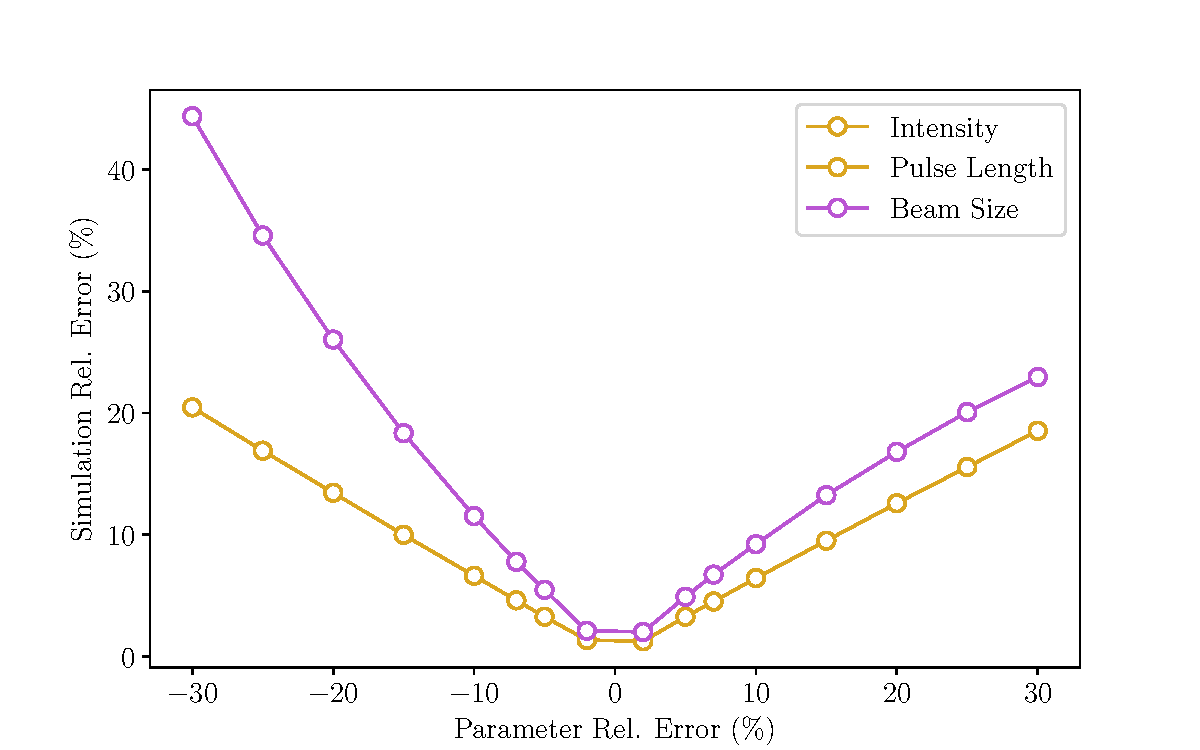
\includegraphics[width=0.7\columnwidth]{BeamParameterUncertainty/BeamParUnc.pdf}
    \caption{Effects of beam parameter uncertainties on maximum temperature simulation results.}
    \label{fig:BeamParUnc}
\end{figure}

It is difficult to give a specific value of the Beam parameters uncertainty, as it is very much dependent on the simulation case. If the range of confidence of the simulation studies is necessary for a certain application a proper study of the Beam parameter uncertainties should be carried out. 

\subsection{Material Parameter Uncertainties.}

Material parameters are all those material properties that are necessary for the simulation. These properties are compiled in Table \ref{tab:MaterialProp}. In most cases, the values of these parameters are well known and can be found in the literature. A very good reference for metallic and non-metallic solids is \parencite[][]{ref:MatProperties}.  

\begin{table}[h]
    \centering
    \begin{tabular}{ccc}
    \hline
    \textbf{Property} & \textbf{Abbreviation} & \textbf{Units} \\ \hline
    Atomic Number     & Z                     &                \\
    Atopic Mass       & A                     & amu            \\
    Density           & rho                   & g/cm3          \\
    Melting Point     & Mp                    & K              \\
    Work Funktion     & phi                   & eV             \\
    Emissivity        & eps                   &                \\
    Specific Heat     & Cp                    & J/gK           \\
    Conductivity      & k                     & W/mK           \\ \hline
    \end{tabular}
    \caption{Material parameters necessary for thermal simulations.}
    \label{tab:MaterialProp}
    \end{table}

Similarly to the beam parameter case, figure  \ref{fig:MatPar} shows the effects uncertainties in the different material parameters have on the final maximum temperature uncertainties. In this case, one can observe how the parameter that induces the highest uncertainty is the specific heat (Cp). How big are the uncertainties is very much dependent on the material. To give a numerical example of typical uncertainty values we studied the Graphite and the tungsten case. 

\begin{figure}[h]
    \centering
    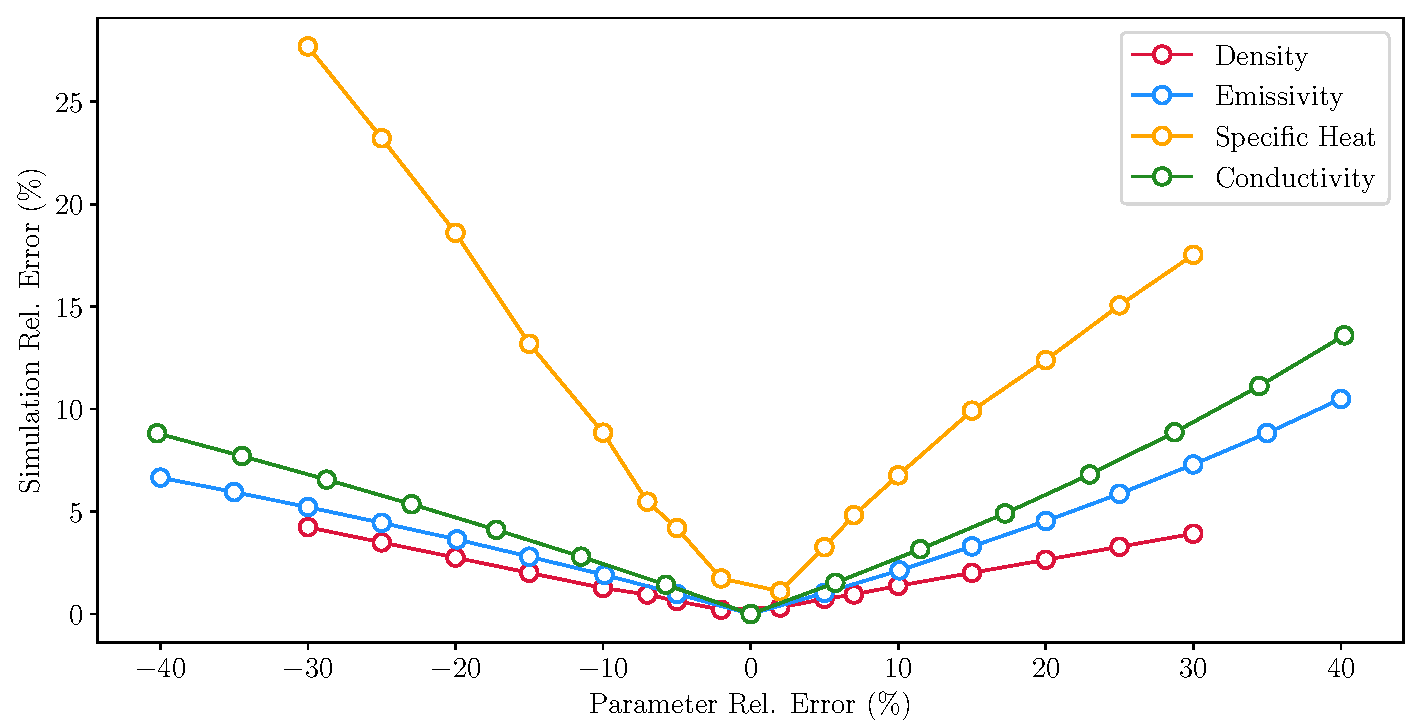
\includegraphics[width=0.7\columnwidth]{MaterialParameterUncertainty/MatParUnc.pdf}
    \caption{Effects of material property uncertainties on maximum temperature results.}
    \label{fig:MatPar}
\end{figure}

Figure \ref{fig:MatPropUnc} shows the uncertainties for specific heat, emissivity and thermal conductivity
parameters for Tungsten and Graphite. In this case, the uncertainties for the other parameters were negligible. This figure was obtained by collecting the values of the material properties reported by different sources. The central points on the boxes represent the average property value, while the limits of the colored boxes represent the RMS. The error bars represent the maximum and minimum discrepancies found with respect to the average value. 

\begin{figure}[h]
    \centering
    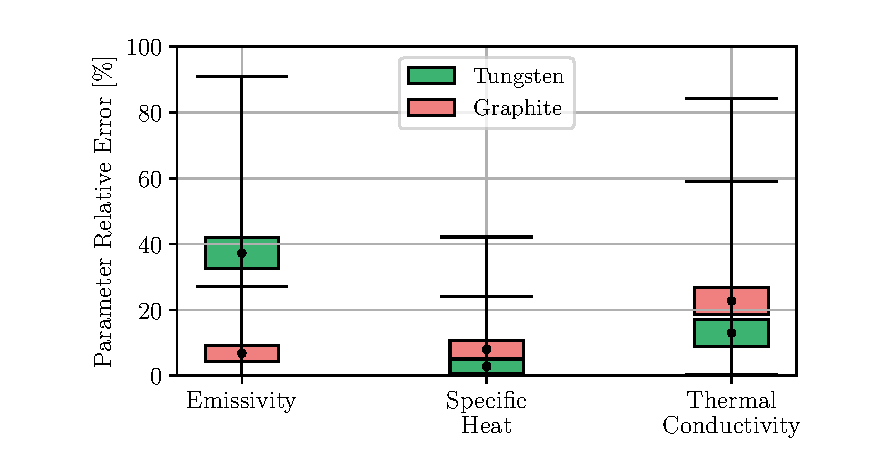
\includegraphics[width=0.7\columnwidth]{PlotTungstenGraphiteUncertainty/GraphTungsUnc.pdf}
    \caption{Material property uncertainties for Graphite and Tungsten. }
    \label{fig:MatPropUnc}
\end{figure}

Uncertainties of the Specific heat are quite small ($2.83 \% $) for both graphite and tungsten. In the case of graphite, values for the emissivity seem to be quite well known ( $ 6.75\%$). Contrarily, a much higher uncertainty was found in the case of its thermal conductivity ( $ 22.71\%$). In the case of tungsten, we find the opposite situation, different sources seem to agree on the value of the thermal conductivity ($13.0\%$ ), however, big uncertainties are found in the emissivity case ($43.26 \%$). 

This big uncertainty in the tungsten emissivity led to an in-depth investigation. To reduce the overall uncertainty of the simulations for tungsten detectors. These experimental measurements and the obtained results will be covered in Chapter \ref{ch:EmissivityMeas}.

\section{Aplications: Beam Power Limit Calculations}

Determining beam power limits means determining beam conditions that could potentially damage the detectors. To do that, the PyTT program was used to simulate the maximum temperatures reached by the detectors for the different expected beam conditions at their location. If the maximum temperature reached was above the safe limit, those beam conditions were considered to be harmful to the detectors. 

\subsection{SEM grid and Slow Wire Stanner at Linac4}

For Linac4, the beam conditions under study were: Beam Intensity ($I_{beam}$), beam pulse length ($\Delta t$) and beam size ($\sigma_x , \sigma_y$). Figure \ref{fig:DetLoc} shows a schematic representation of Linac4, with the different detectors location. The detectors in the L4L, L4D and L4C lines are made of graphite wires ($33 \mu m$). The rest of the wire scanner detectors are also graphite wires, whereas the SEM grid detectors are gold-coated tungsten wires ($40 \mu m$). Table \ref{tab:beamprop} summarizes the range of the beam properties expected at the Linac4 accelerator.

For each detector, a set of dedicated simulations covering the whole parameter range were performed with the PyTT program. A maximum temperature of 1400K was taken as a safe maximum temperature limit. This limit is probably very conservative, as most of the detectors could easily handle up to 3000 K. However, due to the wire-gluing problem suffered in SEM grid detectors, a much lower temperature limit was established. 

\begin{figure}[h]
    \centering
    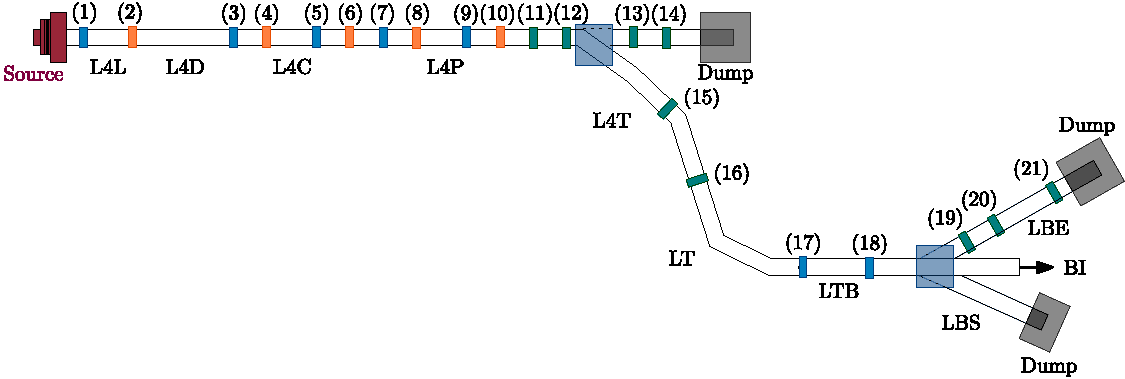
\includegraphics[width=1.0\columnwidth]{Figure_Linac4Instrumetnation/DetecPos.pdf}
    \caption{Schematic representation of Linac4 with SEM grid (blue boxes), wire scanner (orange boxes) locations. Green boxes indicate locations where both, sem grid and wire scanners are installed.}
    \label{fig:DetLoc}
\end{figure}


\begin{table}[h]
    \centering
    \begin{tabular}{cccc}
    \hline
    Property                          & Min & Max & Units   \\ \hline
    Intensity ($I_{beam}$)            & 10  & 25  & mA      \\
    Pulse Length ($\Delta t$)         & 50  & 400 & $\mu s$ \\
    Beam Size ($\sigma_x , \sigma_y$) & 0.5 & 3.0 & mm      \\ \hline
    \end{tabular}
    \caption{Range of beam properties expected at Linac4 accelerator.}
    \label{tab:beamprop}
\end{table}

Figure \ref{fig:EnerCompa} shows an example of the power limits calculated for a detector in L4C line (Detector 5) and a detector at the L4T line (Detector 12). Each square represents the maximum temperature reached by a simulation with the beam pulse length indicated on the X axis, and the beam intensity indicated on the Y axis. The beam size in both cases was $\sigma_x = \sigma_y = 2.0 (mm)$ . 

In both cases, we can observe that beam pulse lengths smaller than 200 $\mu s$ are very safe. Neither detector was getting close to the set temperature limit. One interesting observation is in this case the difference in the results between the detector located at the L4C line and the one located at the L4T line. The only difference between the detectors is the energy deposition in the material. At higher energies, the energy deposition is smaller, so the maximum temperatures reached by the detector are smaller than the equivalent conditions at lower energies. 

\begin{figure}[h]
    \centering
    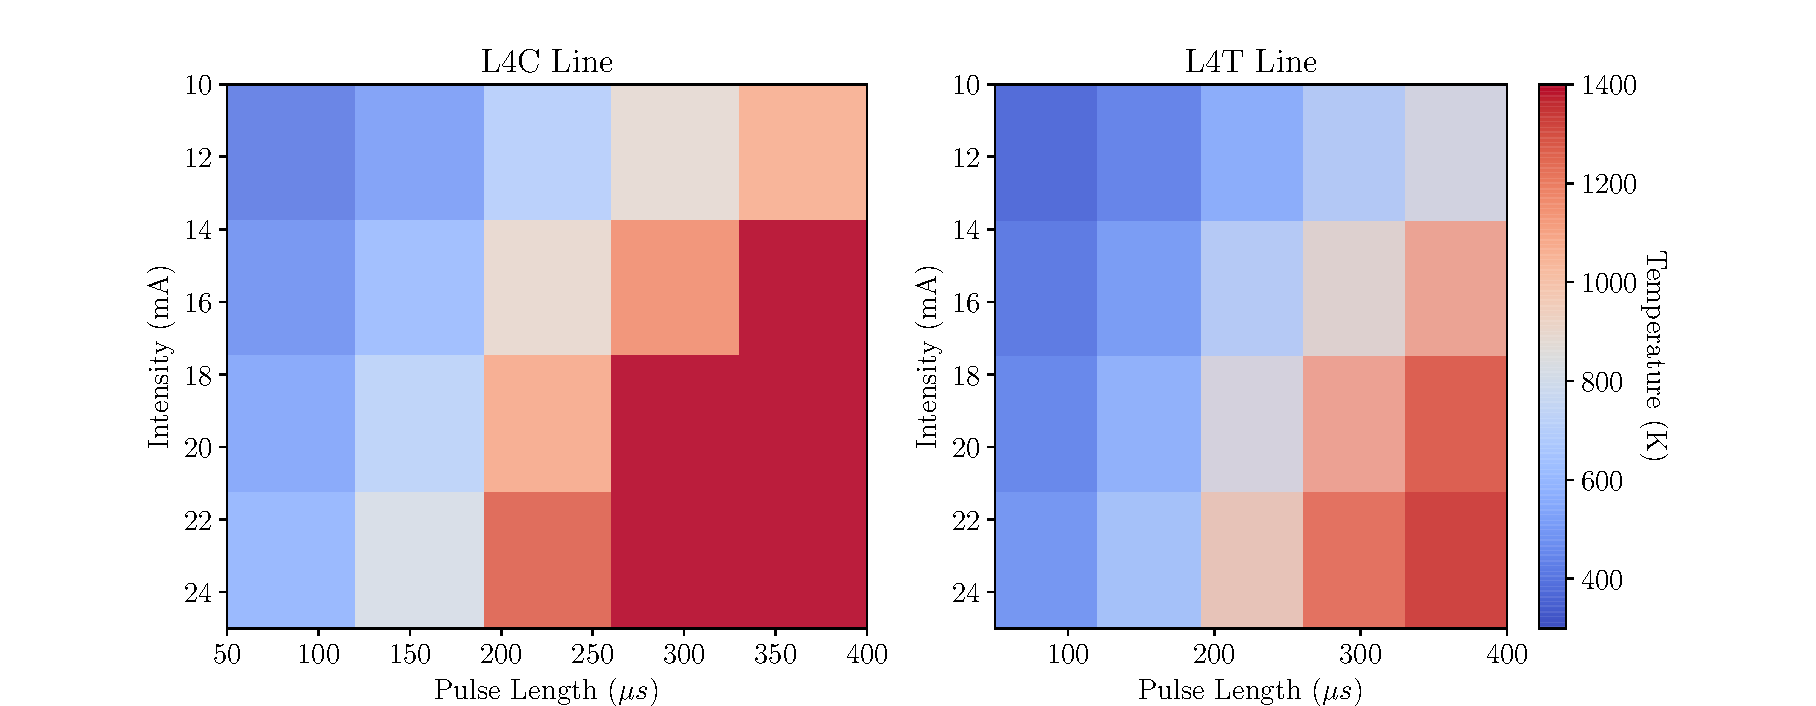
\includegraphics[width=1.0\columnwidth]{Figure_ThermalLimitsSquares/EnergyCompa.pdf}
    \caption{Power limit calculations for a detector at L4C (Left) and a detector at L4T (right) lines. The beam size in both cases was $\sigma_x = \sigma_y = 2.0 (mm)$.}
    \label{fig:EnerCompa}
\end{figure}

Figure \ref{fig:SigmaComparison} shows a similar set of results, but this time, both detectors were placed at locations where the particle energy was already 160 MeV. The difference between the right plot and the left plot is the beam size. The left hand side figure pictures a small beam size ($\sigma_x = 0.8$ (mm), $\sigma_y = 2.0$ (mm)). The right-hand side figure pictures a larger beam size ($\sigma_x = 1.2 (mm)$). From this figure, we can observe how small beam sizes result in much more critical thermal conditions. 

In general, one should be very careful measuring small beam sizes at low energy ranges. An overall power limit for the Linac4 accelerator was established. Beam conditions were considered to be dangerous if the beam size was smaller than 1 $(mm)$ and the beam pulse length was longer than $100 ()\mu s)$. An interlock system for SEM grids and wire scanners was established at Linac4 based on these results. 

\begin{figure}[h]
    \centering
    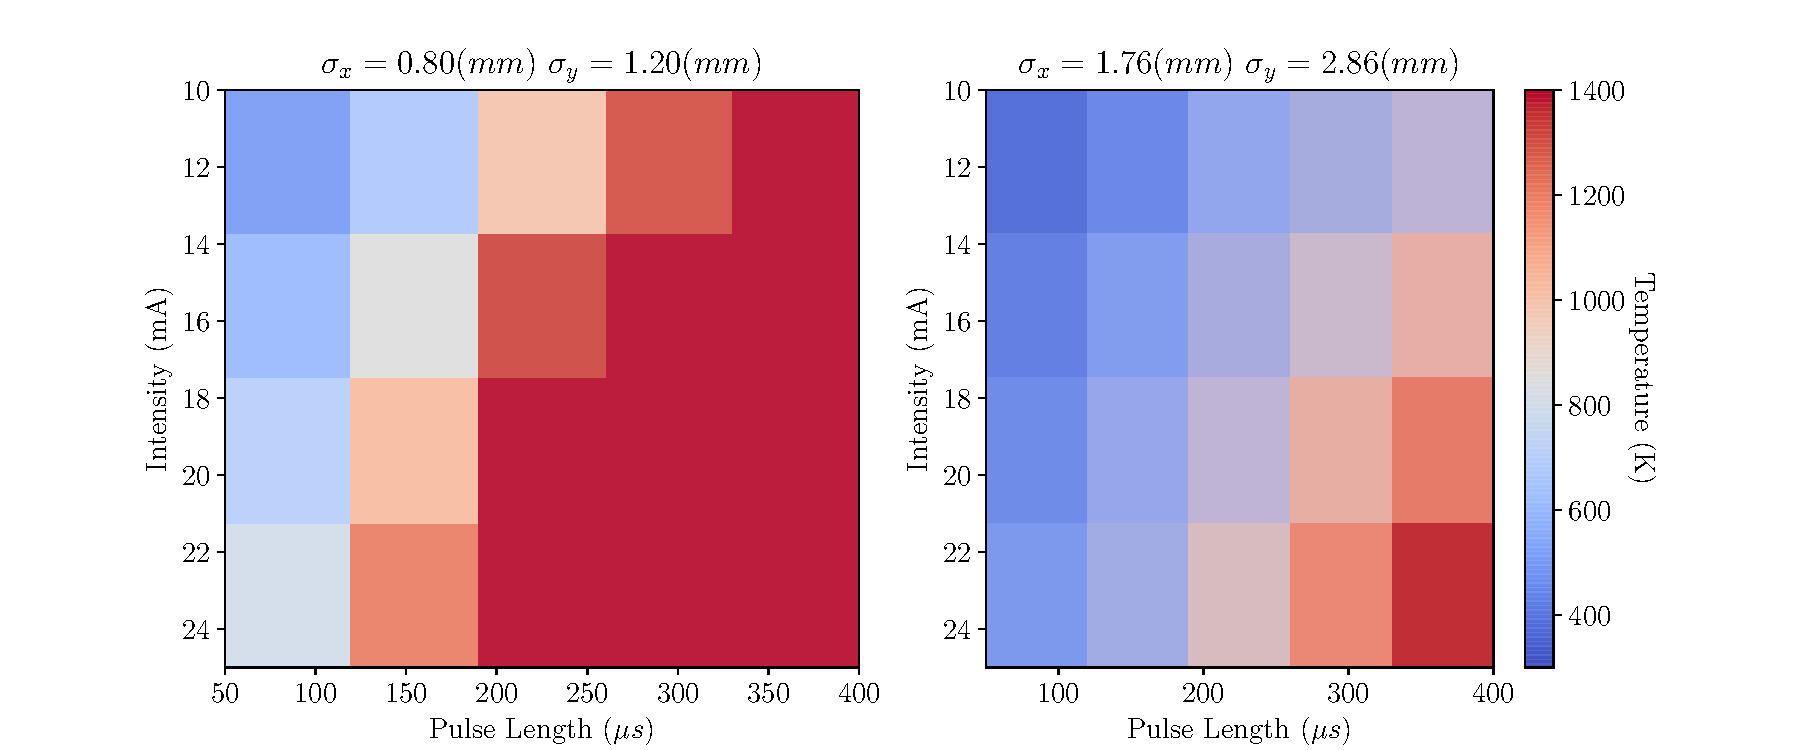
\includegraphics[width=1.0\columnwidth]{Figure_ThermalLimitsSquares/SigmaCompa.pdf}
    \caption{Power limit calculations for a detector at 160 MeV beam energies.}
    \label{fig:SigmaComparison}
\end{figure}

\subsection{Fast Wire Scanners at SPS}

A new generation of beam wire scanners has been developed at CERN, in the framework of the LIU project \parencite[][]{ref:WireScanJose}. In the SPS, 4 new wire scanner systems were installed, for horizontal and vertical beam size measurements. In this case, the relevant parameters under study were: beam emittance (at injection and extraction), the number of protons per bunch (from $10^9$ to $10^{11}$), the maximum number of bunches (from 1 to 288) and wire scanner velocity (form 1 m/s to 20 m/s). 

For the SPS energies ( 26 GeV at injection and 450 GeV at extraction ) differences in energy deposition are not as important as in the Linac4 case. Beam sizes are still a very important parameter to consider. In the SPS, the beam size is usually described in terms of beam emittance. One can easily convert from one to the other with the following relation: 

\begin{equation}
    \sigma = \sqrt{\frac{\epsilon_{norm}}{\gamma_{rel} \cdot \beta_{rel}} \cdot \beta(s)}
\end{equation}

Where $\epsilon_{norm}$ refers to the normalized emittance and $\beta_{rel}$, $\gamma_{rel}$ are the relativistic parameters. $\beta(s)$ is the courant-Snyder parameter at the position s. Because the beam size decreases as the relativistic parameters increase, smaller beam sizes are found in the extraction case. 

Figure \ref{fig:WireScanner1} shows the evolution of the maximum temperature reached by a 33 $\mu m$, graphite, fast wire scanner for a different number of particles per bunch. In this figure, the wire scanner speed was set constant to 1 m/s, and the total number of bunches was always 288.  The figure on the left is for injection energies (26 MeV) and the one on the right is for extraction energies (450 MeV). In both cases, the higher the number of particles per pulse the higher the temperature reached by the detector. 

In these figures, we can also see the decrease of the beam size with the energy, as the temperature increase happens in a much narrower period during extraction energies. 

\begin{figure}[h]
    \centering
    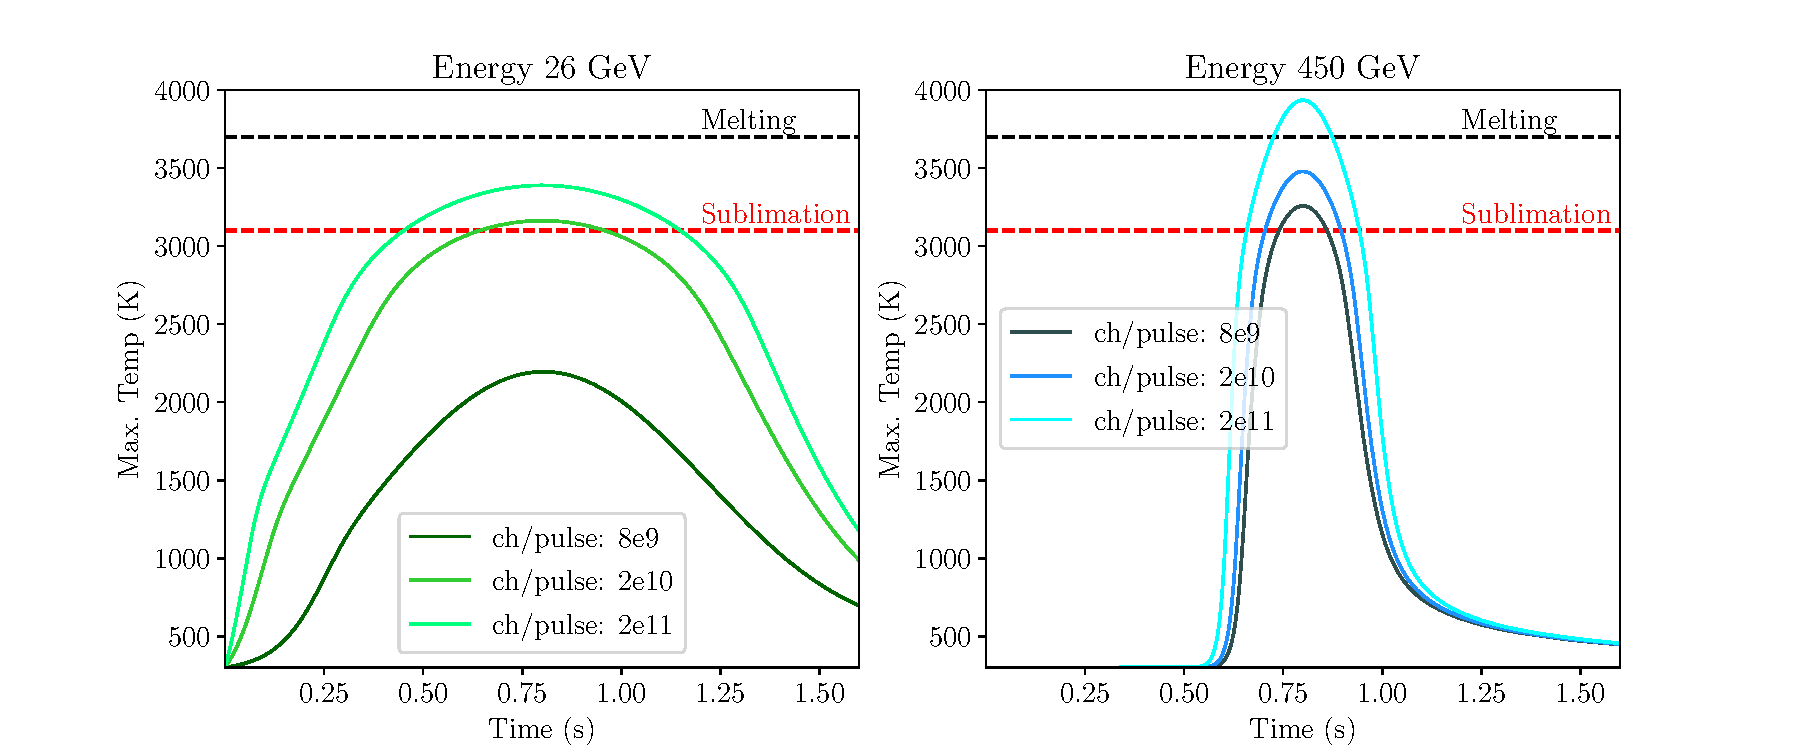
\includegraphics[width=1.0\columnwidth]{WireScanner_Limits/WireLim1.pdf}
    \caption{Comparison of maximum fast wire scanner temperatures reached for different beam conditions. Left: Injection energy. Right: Extraction energy.}
    \label{fig:WireScanner1}
\end{figure}

The wire velocity is also a very important factor to consider. The slower the wire velocity the longer time it will spend in the central area of the beam, and thus the higher the maximum temperature reached. Increasing the wire speed is beneficial in terms of thermal limitations. However, as a tradeoff, we have the measurement resolution. Because the wire scanner in the SPS is much slower than the bunches being accelerated (revolution period $t_{rev} = 2.4\cdot 10^{-5} s$). The number of points per sigma taken by a fast wire scanner can be calculated as: 

\begin{equation}
    n_{points} = \frac{\sigma}{v_{w}\cdot T_{rev}}
\end{equation}

For a beam size of 1 mm, a maximum speed of 10 m/s can be used. Otherwise, the measurements would not have enough resolution. 

The wire damage can be associated with the density of charges traversing the wire \parencite[][]{ref:Msapinski}:

\begin{equation}
     n_{ch} = \frac{N_{ch} \cdot d_{w}}{v_{w} \cdot t_{rev} \cdot \sigma}
\end{equation}

Where $N_{ch}$ is the total number of particles, understood as the number of particles per pulse times the number of pulses. $d_w$ is the wire diameter and $v_w$ is the wire velocity. As a limiting scenario, we could consider the case of a 33 $\mu m$ Graphite wire, with a speed of 1 m/x and measuring a beam size $\sigma_x = \sigma_y = 0.3$ (mm).   In this case the density of particles $n_{ch} = 2.5\cdot 10^{12}$. Beam and wire conditions yielding a charge density higher than this number, are considered to be potentially harmful.

This number is consistent with the experiments performed by M. Sapnski \parencite[][]{ref:Msapinski}. This value is used in the SPS accelerator as a safety limit. Table \ref{tab:MaxNturns} shows an example of how this safety value was used to calculate the maximum number of allowed turns for different wire scanners and beam conditions. At CERN SPS, the maximum number of injected turns can go up to 288. From this table, we can observe that only at injection energies this number of bunches can be measured. 

% Please add the following required packages to your document preamble:
% \usepackage{multirow}
\begin{table}[h]
    \centering
    \begin{tabular}{cclccccc}
    \hline
    \multirow{2}{*}{\begin{tabular}[c]{@{}c@{}}Energy \\ (GeV)\end{tabular}} & \multicolumn{2}{c}{Beam Size (mm)} & \multicolumn{5}{c}{Wire Velocity (m/s)} \\ \cline{2-8}    & $\sigma_x$               & $\sigma_y$              & 1     & 6      & 10    & 15    & 20     \\ \hline
    \multirow{2}{*}{25}                                                      & 3.03             & 2.10            & 54    & 323    & 538   & 807   & 1080   \\
     & 2.0              & 1.38            & 35    & 213    & 350   & 531   & 708    \\ \hline
    \multirow{2}{*}{450}   & 0.72             & 0.50            & 12    & 74     & 129   & 194   & 258    \\    & 0.47             & 0.33            & 8     & 51     & 85    & 127   & 170    \\ \hline
    \end{tabular}
    \caption{Maximum allowed number of beam bunches for different beam conditions. The number of charges per bunch was $1.5 \cdot 10^{11}$ ch/bunch. }
    \label{tab:MaxNturns}
\end{table}

\chapter{Simulation Benchmarking: Thermionic Measurements}
\label{ch:ThermoMeasur}
\pagestyle{fancy}

\graphicspath{ {Figures/Chapter5_SimulationBenchmarking/} }

In this chapter, several different topics will be addressed. The first two sections present the first benchmarking studies for the PyTT simulation tool. Firstly, we present a measurement performed at LINAC4 in which the thermal evolution of the detectors was indirectly measured and compared to the simulations. These measurements were published in \parencite[][]{ref:IBIC2019ARaceli}. Secondly, we present a comparison between the thermal evolution (for thin wires and thin foil) simulated with PyTT and the commercially available software ANSYS. The following sections present three examples of how the PyTT software has been useful for CERN operation. In particular, we show how the PyTT code has been used to calculate beam power limits at LINAC4 and SPS accelerators. 

\section{Thermionic Measurements at LINAC4}
\label{sec:ThAtLINAC4}

The best way to crosscheck the reliability of the thermal evolution simulations introduced in the previous chapter is to compare them with experimental measurements. Many techniques have been developed for measuring the temperature evolution in objects \parencite[][]{ref:ThMeas1}. In our particular case, we were interested in measuring experimentally the temperature evolution of thin wires ($40 \mu m$) during their interaction with the beam of particles. However, no dedicated setup could be installed in any of the CERN machines. The information available was the intensity registered by the SEM Grids and wire scanners along the LINAC4 accelerator. One can correlate the current measured to the temperature thanks to the thermionic emission process. 

As explained in Chapter \ref{ch:BeamMatterInter}, Section \ref{sec:ThermoCurrent}, Thermionic emission current ($J_{th}$) is negligible at low temperatures but it becomes considerable when higher temperatures are reached. The idea for these measurements was to find certain beam conditions that allowed us to reach high temperatures and thus register the thermionic current. Due to the close relationship between the thermionic current and the temperature, by comparing the simulated current and the experimentally measured one, we could judge the reliability of our thermal simulation results. 

\subsection{Experimental Planning}

For normal beam conditions, the currents measured by the individual wires in SEM grid, or the single wire in a Wire Scanner, are around 1 (mA). For the experimental planning, a signal was considered detectable if the thermionic current was higher than 0.05 (mA). Figure \ref{fig:ThermCurrent} shows the expected current generated, by thermionic emission, in a Tungsten (40$\mu m$) and a Graphite (33 $\mu m$) wire as a function of the wire temperature. From this figure, one can observe that temperatures above 2100 (K) will be required to obtain a detectable thermionic current.  
\begin{figure}[h]
    \centering
    \includegraphics[width=1.0\columnwidth]{Figure_ThermoionicCurrent/ThermoCurrent.pdf}
    \caption{Thermionic current as a function of the temperature for Tungsten (40$\mu m$) and a Graphite (33 $\mu m$) wires.}
    \label{fig:ThermCurrent}
\end{figure}
\begin{figure}[h!]
    \centering
    \includegraphics[width=1.0\columnwidth]{Linac4Instrumetnation/Linac4Instruments.pdf}
    \caption{Schematic representation of Linac4 layout, with locations of the SEM Grid (L4T.BSGH/V.0243) and the BCT (L4T.BCT.0107) used for thermionic measurements.}
    \label{fig:DetLocation}
\end{figure}

Due to the high temperatures needed for performing the measurements, the risk of permanent detector damage was non-negligible. Only those detectors with already existing damage, or those placed in areas where it was planned to open vacuum. After some deliberation, it was decided that the SEM grid L4T.BSGH/V.0243, would be used for the measurements. The beam current transformer L4T.BCT.0107 was used for continuous intensity and pulse length measurements. These detectors are located at LINAC4 in the L4T line. The position of these detectors is shown in figure \ref{fig:DetLocation}. 

\begin{table}[h]
    \centering
    \begin{tabular}{cccc}
    \hline
    Pitch   & \# of Wires & Wire Distance (mm) & Covered Region (mm) \\ \hline
    \multirow{5}{*}{3} & 6 + 6 = 12  & 0.4                & 4.4                 \\
                       & 3 + 3 = 6   & 0.75               & 8.9                 \\
                       & 3+3 = 6     & 1.0                & 14.9                \\
                       & 2 + 2 = 4   & 2.5                & 24.9                \\
                       & 2 + 2 = 4   & 4.0                & 40.9                \\ \hline
    \end{tabular}
    \caption{Detailed description of wire location in SEM grid L4T.BSGH/V.0243}
    \label{tab:WireSpacing}
\end{table}
\begin{figure}[h]
    \centering
    \includegraphics[width=1.0\columnwidth]{Figure_SemGridSchema/SemGridSchema.pdf}
    \caption{Schematic representation of wire position at L4T.BSGH/V.0243. }
    \label{fig:WireSpacing}
\end{figure}

The SEM grid used for the measurement was conformed of 32 Tungsten wires with gold coating. The wires had a length of 5 (cm) and a thickness of 40 $(\mu m)$. The wires were unevenly spaced, covering a total area of 40.9 (mm). Table \ref{tab:WireSpacing} details the locations of the different wires. The wires were placed on the top and the bottom part of the frame alternatively as shown in figure \ref{fig:WireSpacing}.

\begin{figure}[h]
    \centering
    \includegraphics[width=1.0\columnwidth]{Figure_IsThereThermo/IsThereThermo.pdf}
    \caption{Summary of expected maximum current for different beam conditions. Gray Area indicates where thermionic emission is detectable. The beam size is given in (mm) and Beam intensity in (mA).}
    \label{fig:Jth_Cond}
\end{figure}

A preliminary study was performed to determine what kind of beam parameters would potentially yield a detectable thermionic current. In the L4T line, the energy of the \hm beam of particles is already 160 MeV. The beam parameters that could be easily adjusted to convenienceare: Beam intensity ($I_{beam}$), beam pulse length ($\Delta_t$), and beam size ($\sigma_x , \sigma_y$). Figure \ref{fig:Jth_Cond} shows a summary of the maximum expected thermionic current for different beam conditions. 

From this figure one can observe, that large beam sizes ($\sigma_x$ = $\sigma_y$ = 2 mm) will not yield detectable thermionic emission. For smaller beam sizes ($\sigma_x \leq \sigma_y \leq 1$ mm), thermionic emission can be detected for long beam pulse lengths ($\Delta t > 300 $ $\mu s$). Setting up the beam size to a specific dimension is not an easy task. Changes in the intensity of the beam also didn't produce very dramatic changes in the detectable current. During the measurements, these two quantities were kept constant while the beam pulse length was systematically increased in order to reach the thermionic stage in a controlled way. 

\subsection{Experimental Results}

The first set of measurements was taken using conservative beam conditions. The intensity of the beam was kept constant to $I_{beam} = 17.30 (17)$ mA. The beam size was $\sigma_x = 1.02(5) $ mm and $\sigma_y = 1.76(2)$ mm, with the beam centered at $\mu_x = -0.22(6)$ mm and $\mu_y = -0.43(21)$ mm. Figure \ref{fig:PulseEvol} shows the evolution of the beam size and position during a LINAC4 pulse. During these measurements, the beam pulse length was varied between $\Delta t = 165.38(48)$ $\mu s$ up to $\Delta t = 247.12(33)$ $\mu s$. As expected, no sign of thermionic emission was observed. However, when the long beam pulse lengths were measured, wires 15 and 17 were glued together. Figure \ref{fig:WireGlued} shows the current registered by the different wires of the grid as a function of time for four consecutive beam pulses. 

\begin{figure}[h]
    \centering
    \includegraphics[width=1.0\columnwidth]{Figure_BeamProfileStudy/BeamProfEvol1.pdf}
    \caption{Evolution of the transverse beam profile along the beam pulse. Top: example of transverse beam profile measurement. Bottom: Calculated beam size from gaussian approximation. Error bars were calculated by measuring different beam pulses.  }
    \label{fig:PulseEvol}
\end{figure}

In order to avoid this situation and proceed with the measurements, the beam of particles was steered away from these wires and centered around $\mu_x = -1.89(11)$  $mm$ and $\mu_y = 1.15(31)$ $mm$. The wire separation in this position is much larger, making wire gluing more challenging. The horizontal beam size was reduced to $\sigma_x = 0.59(17) mm$. As a result the vertical plane grew longer, $\sigma_y = 3.23(54)$ $mm$. During these measurements, the beam intensity was slightly smaller $I_{beam} \sim 16.7$ $mA$. The beam pulse length was increased systematically until thermionic emission was observed. On the vertical grid, Thermionic emission was observable in various wires for a beam pulse length of $\sim 450$ $\mu s$. 

\begin{figure}[h]
    \centering
    \includegraphics[width=1.0\columnwidth]{Figure_WiresGluing/WireWithTime.pdf}
    \caption{Evolution of the measured current in different wires as a function of time, for six consecutive beam pulses. }
    \label{fig:WireGlued}
\end{figure}
\begin{figure}[h!]
    \centering
    \includegraphics[width=1.0\columnwidth]{Figure_ThermionicMeasurements/VerticalThermoCurrent.pdf}
    \caption{Current registered by several wires during the beam pulse. The units of the signals are (ADC counts).}
    \label{fig:MeasuredThermo}
\end{figure}

Figure \ref{fig:MeasuredThermo} shows the current measured by several wires in the vertical SEM grid during the beam passage. When the particles reached the detector a negative signal is registered. As time goes by, the energy deposition in the detector material rises the temperature of the detector. As temperature increases, thermionic emission increases, and one can observe this increase in the reduction of the absolute value of the current. Once the particle beam has disappeared, a small positive current remains. Because the detector is still warm, thermionic emission current is still being registered.  As the detector cools down, this current diminishes. 

In figure \ref{fig:MeasuredThermo} one can also observe some fluctuations in the registered beam current. This was an effect of the particle beam of particles itself, and could also be observed in the BCT measurements. Also, at $t = 250 \mu s$ and $t = 400 \mu s$, an anomalous value of the beam current is registered by all the wires. To avoid injection losses due to in-between rings injection, the Linac4 chopper removes part of the Linac4 beam every 150 $\mu s$. Which explains the intensity jumps registered by the wires. The intensity fluctuations and gaps at 250 $\mu s$ and 400 $\mu s$, are intrinsic to the particle beam and could also be measured by the BCT. 

The effects of thermionic emission can be also observed in the beam profile measurements. This is shown in figure \ref{fig:JthInProf}. In this figure, lighter currents indicate profiles taken at larger times during the beam pulse. We can see how the beam profile measurements are affected by the thermionic current.

\begin{figure}[h]
    \centering
    \includegraphics[width=1.0\columnwidth]{Figure_ThermionicMeasurements/ProfileJth.pdf}
    \caption{Example of vertical profile beam measurement. Darker colors indicate measurements at the beginning of the beam shot. Lighter colors indicate measurements a the end of the shot. }
    \label{fig:JthInProf}
\end{figure}

\subsection{Measurment-Simulation Comparison}

% PyTT program was used to simulate the thermal and electrical evolution of the detectors during the measurements. For the simulations, the intensity of the beam was considered to be constant. Intra-pulse intensity fluctuations and chopper effects were not considered. Figure \ref{fig:MeasSimCompa} shows a comparison between the signal measured by wire 19 of the SEM grid, the simulated current, and the current measured by BCT.0107. The BCT intensity has been included in the comparison to show the intrinsic properties of the beam. The BCT signal clearly shows when the Beam pulse starts and ends. It also shows the aforementioned beam intensity fluctuations and the chopper gaps. However, the current reduction at longer beam pulse time is not observable in the BCT measurements, as this is an effect occurring on the wire. 

% \begin{figure}[h]
%     \centering
%     \includegraphics[width=1.0\columnwidth]{Figure_MeasurementSimulationCompa/VerticalCompa.pdf}
%     \caption{Signal generated in the wire intercepting the beam as a function of time. Compared with simulated intensity results. }
%     \label{fig:MeasSimCompa}
% \end{figure}

%  Also, the positive current used by the wire after the beam pulse has passed is not observable in the BCT signal. This means the current measured by the detector at that time does not come from the beam. The simulation results seem to very clearly reproduce the average of the measured SEM current. The simulations show a slightly slower start for the thermionic emission current. However, after the beam pulse is gone, the simulated and the measured results for the thermionic current match very well. 

% The maximum relative error between simulated and measured results is found to be around 30 $\%$, and it is found at the very end of the beam shot. Even then, the average relative error along the whole pulse is $6.3(25) \%$. 

% A dedicated uncertainty study was performed to determine the uncertainties of the simulated results (See Section \ref{sec:ModelUnc}). In this particular case, the biggest contributor to the simulation's uncertainty came from uncertainties in the beam size. As indicated in the previous section, the beam size was $\sigma_x = 0.59(17)$ mm and $sigma_y = 3.23(54)$ mm. This implies, beam size uncertainty was $\xi_x = 28.81 \%$ and $\xi_y = 16.71 \%$. As shown in section \ref{sec:ModelUnc}, uncertainties in beam sizes can yield big uncertainties in simulation results, mainly when small beam sizes are involved. 

% As we saw in figure \ref{fig:MeasuredThermo}, several wires measured thermionic emission. However, due to the small changes in the measured intensity between the different wires and the big uncertainties in the simulated results, it was impossible to distinguish among them. 


% \section{Simulation Comparison: Ansys}
% \label{sec:AnsysComparison}

% The objective of this study was to compare the results obtained with the PyTT code, with results obtained with Ansys, a highly used and benchmarked commercially available software. 

% For this work, the theory of finite differences (FDM) has been used to solve the heat equation, as was explained in Chapter \ref{ch:TempModeling}. However, FDM is just an example of a numerical technique to solve PDEs and it is important to stress that alternative approaches abound. Commercially available softwares, such as Ansys \parencite[][]{ref:Ansys}, are commonly used to accurately solve a big variety of multiphysics phenomena. In particular, Ansys uses Finite Element Analysis (FEA) \parencite[][]{ref:NumericalMethodBook} to aid the users obtain solutions for real engineering problems. 

% \subsection{Thin Wire Studies}

% The first part of this study compares the thermal evolution results, of a thin tungsten wire ($\phi$ = 40 $\mu m$), calculated with the PyTT code and Ansys. Here, a LINAC4-like beam of particles was considered as the heating source. Table \ref{tab:BeamParametersCompa} summarizes the parameters of the beam. The parameters on this table remained constant for all the simulations. The beam pulse length was systematically varied to cover different temperature ranges. 

% \begin{table}[h]
%     \centering
%     \begin{tabular}{ccccc}
%     \hline
%     Particle & \begin{tabular}[c]{@{}c@{}}Energy\\ (MeV)\end{tabular} & \begin{tabular}[c]{@{}c@{}}Inensity\\ (mA)\end{tabular} & \begin{tabular}[c]{@{}c@{}}Sigma x \\ (mm)\end{tabular} & \begin{tabular}[c]{@{}c@{}}Sigma y\\ (mm)\end{tabular} \\ \hline
%     Proton   & 160   & 25      & 0.5           & 1.                        \\ \hline
%     \end{tabular}
%     \caption{Summary of the beam parameters that remained constant during the simulations.}
%     \label{tab:BeamParametersCompa}
% \end{table}

% \begin{figure}[h]
%     \centering
%     \includegraphics[width=1.0\columnwidth]{HeatInpuCompa/HeatInputCompa.pdf}
%     \caption{Examples of the heat flux provided to Ansys and PyTT for three different simulation cases.}
%     \label{fig:AppliedHeatWire}
% \end{figure}

% To achieve the closes simulation conditions, a cuboid approximation of the wire was considered in both, PyTT and Ansys. The wire was oriented along the y-axis, with a wire length of 2 (cm). The spatial mesh resolution was 0.1 (cm) along the wire length and for the x and z directions a single mesh element was considered. The temporal resolution was divided into two sections. During the beam pulse, temporal elements of $10^{-7}$ (s) were considered, while during the cooling section the temporal elements were $10^{-4}$ (s) long. Material parameters, such as heat capacity and conductivity, were considered to be temperature-dependent. However, the emissivity was considered to be constant and equal to 0.1 in both cases. 

% In Ansys, the heat load was given using APDL commands \parencite[][]{ref:APDLCommand}. Here, a gaussian distribution with the heat flux ($W/m^2$) equivalent of a beam pulse was described and applied to the material surface. Figure \ref{fig:AppliedHeatWire} shows the heat flux applied to the wire by both Ansys and PyTT. The heat load in PyTT is constant during the presence of the beam pulse, and it immediately goes to zero once the beam pulse has passed. In the case of Ansys, a more smooth heat load transition is observed. The total integrated heat flux was the same in both programs, with a maximum discrepancy of $0.64\%$ for the shorter beam pulses ($\Delta t \leq 50$ $\mu s$). 

% Figure \ref{fig:TemperatureComparison} compares the evolution of the maximum temperature, for three different beam pulse lengths, as a function of time. In these figures, one can observe how the PyTT simulations systematically give a higher maximum temperature than the results obtained with Ansys. The cooling rate in the PyTT code seemed to be slightly slower than in Ansys. The maximum discrepancy between the Ansys and the PyTT results was $11.2\%$ for a temperature of 1356K. 

% \begin{figure}[h]
%     \centering
%     \includegraphics[width=1.0\columnwidth]{TempCompa/TempCompa.pdf}
%     \caption{Comparison of the evolution of the maximum temperature in the detector as a function of time, for three different beam pulse lengths.}
%     \label{fig:TemperatureComparison}
% \end{figure}

% One big difference between these two programs when performing this study was the simulation time. PyTT averaged 10.56 (s) when performing these simulations, while Ansys averaged 7:35 (min), in a Hp Intel(R) Core(TM) i7-6700 CPU, 16.0 Go RAM. This comparison might not be fair, Ansys is a much more complex simulation tool, with many many more options and accurate models. Also with the appropriate knowledge, the simulation times can be optimized. However, if what is important is to quickly obtain a number that can give the user if certain beam parameters are going to damage or not a detector, the PyTT code can manage to do it fast, with results that are very similar to the ones obtained with Ansys. 

% \subsection{Thin Foil Studies}

% Similar Studies were performed with thin graphite foils ( dimensions = 2 (cm) x 2 (cm) x 40 ($\mu m$)). The beam conditions for this study were the same as the ones described in table \ref{tab:BeamParametersCompa}. Variations on the beam pulse length were used again to control the maximum temperature reached by the detectors. 

% \begin{figure}[h]
%     \centering
%     \includegraphics[width=0.9\columnwidth]{ErrorCompa/FoilMaxTempCompa.pdf}
%     \caption{Comparison of the evolution of the maximum temperature in $40 \mu m$ graphite foil, as a function of beam pulse length. On the right axis, the relative error between them is represented. }
%     \label{fig:TempMaxErrCompa} 
% \end{figure}
% \begin{figure}[h]
%     \centering
%     \includegraphics[width=0.9\columnwidth]{CoolingSpeedAnsys/CoolingSpeed.pdf}
%     \caption{Comparison of the cooling rate between PyTT code and Ansys. For a $40 \mu m$ graphite foil after a beam shot. }
%     \label{fig:CoolingRate} 
% \end{figure}

% Figure \ref{fig:TempMaxErrCompa} shows the maximum temperature reached (at equilibrium), with both PyTT and Ansys codes, as a function of the beam pulse length. From this figure, one can see how at higher temperatures PyTT continues to systematically give a higher maximum temperature. However, at lower temperatures, Ansys gives higher temperature results. The relative error between the Ansys and PyTT results is higher at lower beam pulse lengths, however, it never exceeds a $20 \%$.

% For a beam pulse length of $100$ $\mu s$, the cooling rate was calculated with Ansys and with PyTT. Figure \ref{fig:CoolingRate} shows a comparison between the cooling rate after a beam shot. From this figure, we can observe how Ansys presented a much faster cooling at the beginning (higher temperatures) and a slower cooling after some time (lower temperatures). Here, the temperature right after the beam shot was 848 (K).

% Another interesting feature we wanted to compare was the heat distribution in space. Figure \ref{fig:FancyPlotComparison} shows the heat distribution of the foil simulated with Ansys (left) and the PyTT code (right). These two figures were taken at the same instant of time (10 ms after beam shot arrival), during the cooling process. It is clear from these pictures that the heat distribution is very similar in both cases. It is very difficult to properly understand the differences between these results. Information about the numerical methods employed by Ansys is not publicly available. So no more quantitative or in-depth conclusions could be taken from these studies. 

% \begin{figure}[h]
%     \centering
%     \begin{subfigure}[b]{0.6\textwidth}
%         \centering
%         \includegraphics[width=\textwidth]{AnsysPyTT_2Dcompa/Ansys2DPlot.png}
%     \end{subfigure}
%     \hfill
%     \begin{subfigure}[b]{0.8\textwidth}
%         \centering
%         \includegraphics[width=\textwidth]{AnsysPyTT_2Dcompa/FoilPyTT.pdf}        
%     \end{subfigure}

%     \caption{Comparison between thermal distribution in Graphite foil after one beam shot. In Ansys (top) and PyTT code (bottom). The black lines in Ansys have a separation of 1 mm.}

%      \label{fig:FancyPlotComparison} 
% \end{figure}

% \section{Beam Power Limit Calculations}

% Determining beam power limits means determining beam conditions that could potentially damage the detectors. To do that, the PyTT program was used to simulate the maximum temperatures reached by the detectors for the different expected beam conditions at their location. If the maximum temperature reached was above the safe limit, those beam conditions were considered to be harmful to the detectors. 

% \subsection{SEM grid and Slow Wire Stanner at Linac4}
% \label{sec:BeamPowerL4}

% For Linac4, the beam conditions under study were: Beam Intensity ($I_{beam}$), beam pulse length ($\Delta t$) and beam size ($\sigma_x , \sigma_y$). Figure \ref{fig:DetLocation} shows a schematic representation of Linac4, with the different detectors location. The detectors in the L4L, L4D and L4C lines are made of graphite wires (33 $\mu m$). The rest of the wire scanner detectors are also graphite wires, whereas the SEM grid detectors are gold-coated tungsten wires (40 $\mu m$). Table \ref{tab:beamprop} summarizes the range of the beam properties expected along the Linac4 accelerator.

% For each detector, a set of dedicated simulations covering the whole parameter range were performed with the PyTT program. A maximum temperature of 1400K was taken as a safe maximum temperature limit. This limit is probably very conservative, as most of the detectors could easily handle up to 3000 K. However, due to the wire-gluing problem suffered in SEM grid detectors, due to gold coating, a much lower temperature limit was established. 

% \begin{table}[h]
%     \centering
%     \begin{tabular}{cccc}
%     \hline
%     Property                          & Min & Max & Units   \\ \hline
%     Intensity ($I_{beam}$)            & 10  & 25  & mA      \\
%     Pulse Length ($\Delta t$)         & 50  & 400 & $\mu s$ \\
%     Beam Size ($\sigma_x , \sigma_y$) & 0.5 & 3.0 & mm      \\ \hline
%     \end{tabular}
%     \caption{Range of beam properties expected at Linac4 accelerator.}
%     \label{tab:beamprop}
% \end{table}

% Figure \ref{fig:EnerCompa} shows an example of the power limits calculated for a detector in L4C line (Detector 5) and a detector at the L4T line (Detector 12). Each square represents the maximum temperature reached by a simulation with the beam pulse length indicated on the X-axis, and the beam intensity indicated on the Y-axis. The beam size in both cases was $\sigma_x = \sigma_y = 2.0$ mm. In both cases, we can observe that beam pulse lengths smaller than 200 $\mu s$ are very safe. Neither detector was getting close to the set temperature limit. The only difference between the detectors is the energy deposition in the material. At higher energies, the energy deposition is smaller, so the maximum temperatures reached by the detector are smaller than the equivalent conditions at lower energies. 

% Figure \ref{fig:SigmaComparison} shows a similar set of results, but this time, both detectors were placed at locations where the particle energy was already 160 MeV. The difference between the right plot and the left plot is the beam size. The left-hand side figure pictures a small beam size. The right-hand side figure pictures a larger beam size. From this figure, we can observe how small beam sizes result in much more critical thermal conditions. 

% In general, one should be very careful measuring small beam sizes at low energy ranges. An overall power limit for the Linac4 accelerator was established. Beam conditions were considered to be dangerous if the beam size was smaller than 1 $(mm)$ and the beam pulse length was longer than $100 ()\mu s)$. An interlock system for SEM grids and wire scanners was established at Linac4 based on these results. 

% \begin{figure}[h]
%     \centering
%     \includegraphics[width=1.0\columnwidth]{Figure_ThermalLimitsSquares/EnergyCompa.pdf}
%     \caption{Power limit calculations for a detector at L4C (Left) and a detector at L4T (right) lines. The beam size in both cases was $\sigma_x = \sigma_y = 2.0$ mm.}
%     \label{fig:EnerCompa}
% \end{figure}

% \begin{figure}[h]
%     \centering
%     \includegraphics[width=1.0\columnwidth]{Figure_ThermalLimitsSquares/SigmaCompa.pdf}
%     \caption{Power limit calculations for a detector at 160 MeV beam energies.}
%     \label{fig:SigmaComparison}
% \end{figure}

% \subsection{Fast Wire Scanners at SPS}
% \label{sec:BeamPowerSPS}

% A new generation of beam wire scanners has been developed at CERN, in the framework of the LIU project \parencite[][]{ref:WireScanJose}. In the SPS, 4 new wire scanner systems were installed, for horizontal and vertical beam size measurements. In this case, the relevant parameters under study were: beam emittance (at injection and extraction), the number of protons per bunch (from $10^9$ to $10^{11}$), the maximum number of bunches (from 1 to 288) and wire scanner velocity (form 1 m/s to 20 m/s). 

% For the SPS energies ( 26 GeV at injection and 450 GeV at extraction ) differences in energy deposition are not as important as in the Linac4 case. Beam sizes are still a very important parameter to consider. In the SPS, the beam size is usually described in terms of beam emittance. One can easily convert from one to the other with the following relation: 

% \begin{equation}
%     \sigma = \sqrt{\frac{\epsilon_{norm}}{\gamma_{rel} \cdot \beta_{rel}} \cdot \beta(s)}
% \end{equation}

% Where $\epsilon_{norm}$ refers to the normalized emittance and $\beta_{rel}$, $\gamma_{rel}$ are the relativistic parameters. $\beta(s)$ is the courant-Snyder parameter at the position s. However, because the beam size decreases as the relativistic parameters increase, smaller beam sizes are found in the extraction case. 

% \begin{figure}[h]
%     \centering
%     \includegraphics[width=1.0\columnwidth]{WireScanner_Limits/WireLim1.pdf}
%     \caption{Comparison of maximum fast wire scanner temperatures reached for different beam conditions. Left: Injection energy. Right: Extraction energy.}
%     \label{fig:WireScanner1}
% \end{figure}

% Figure \ref{fig:WireScanner1} shows the evolution of the maximum temperature reached by a 33 $\mu m$, graphite, fast wire scanner for a different number of particles per bunch. In this figure, the wire scanner speed was set constant to 1 m/s, and the total number of bunches was always 288.  The figure on the left is for injection energies (26 MeV) and the one on the right is for extraction energies (450 MeV). In both cases, the higher the number of particles per pulse the higher the temperature reached by the detector. In these figures, we can also see the decrease of the beam size with the energy, as the temperature increase happens in a much narrower period during extraction energies. 

% The wire velocity is also a very important factor to consider. The slower the wire velocity the longer time it will spend in the central area of the beam, and thus the higher the maximum temperature reached. Increasing the wire speed is beneficial in terms of thermal limitations. However, as a tradeoff, we have the measurement resolution. Because the wire scanner in the SPS is much slower than the bunches being accelerated (revolution period $t_{rev} = 2.4\cdot 10^{-5} s$). The number of points per sigma taken by a fast wire scanner can be calculated as: 

% \begin{equation}
%     n_{points} = \frac{\sigma}{v_{w}\cdot T_{rev}}
% \end{equation}

% For a beam size of 1 mm, a maximum speed of 10 m/s can be used. Otherwise, the measurements would not have enough resolution. The wire damage can be associated with the density of charges traversing the wire \parencite[][]{ref:Msapinski}:

% \begin{equation}
%      n_{ch} = \frac{N_{ch} \cdot d_{w}}{v_{w} \cdot t_{rev} \cdot \sigma}
% \end{equation}

% Where $N_{ch}$ is the total number of particles, understood as the number of particles per pulse times the number of pulses. $d_w$ is the wire diameter and $v_w$ is the wire velocity. As a limiting scenario, we could consider the case of a 33 $\mu m$ Graphite wire, with a speed of 1 m/s and measuring a beam size $\sigma_x = \sigma_y = 0.3$ mm. In this case the density of particles $n_{ch} = 2.5\cdot 10^{12}$. Beam and wire conditions yielding a charge density higher than this number, are considered to be potentially harmful.

% This number is consistent with the experiments performed by M. Sapnski \parencite[][]{ref:Msapinski}. This value is used in the SPS accelerator as a safety limit. Table \ref{tab:MaxNturns} shows an example of how this safety value was used to calculate the maximum number of allowed turns for different wire scanners and beam conditions. At CERN SPS, the maximum number of injected turns can go up to 288. From this table, we can observe that only at injection energies this number of bunches can be measured. 

% \begin{table}[h]
%     \centering
%     \begin{tabular}{cclccccc}
%     \hline
%     \multirow{2}{*}{\begin{tabular}[c]{@{}c@{}}Energy \\ (GeV)\end{tabular}} & \multicolumn{2}{c}{Beam Size (mm)} & \multicolumn{5}{c}{Wire Velocity (m/s)} \\ \cline{2-8}    & $\sigma_x$               & $\sigma_y$              & 1     & 6      & 10    & 15    & 20     \\ \hline
%     \multirow{2}{*}{25}                                                      & 3.03             & 2.10            & 54    & 323    & 538   & 807   & 1080   \\
%      & 2.0              & 1.38            & 35    & 213    & 350   & 531   & 708    \\ \hline
%     \multirow{2}{*}{450}   & 0.72             & 0.50            & 12    & 74     & 129   & 194   & 258    \\    & 0.47             & 0.33            & 8     & 51     & 85    & 127   & 170    \\ \hline
%     \end{tabular}
%     \caption{Maximum allowed number of beam bunches for different beam conditions. The number of charges per bunch was $1.5 \cdot 10^{11}$ ch/bunch. }
%     \label{tab:MaxNturns}
% \end{table}



\chapter{Thin Wire Emissivity Measurements}
\label{ch:EmissivityMeas}
\pagestyle{fancy}

\graphicspath{ {Figures/Chapter6_EmissivityMeasurement/} }

\section{Motivation}

In chapter \ref{ch:TempModeling}, we saw that material properties such as melting (or sublimating) temperatures, heat capacity, thermal conductivity, emissivity, etc. play a very important role in properly describing the thermal behavior and limitations of our detectors. Uncertainties in these values yielded uncertainties in the final simulated results. The highest material parameter uncertainty was found in the case of the tungsten emissivity, showing an average uncertainty of around $43.26 \%$.

Figure \ref{fig:EmissUnc} tries to break down this uncertainty value in more detail. In this figure, every curve represents the emissivity value (as a function of the temperature) reported by a different source. A summary of all these sources and their corresponding reference can be found in \parencite[]{ref:MatProperties}. From this figure we can observe the big spread of the emissivity value reported by the different sources, covering almost all the available ranges (0 - 1). 

\begin{figure}[h]
    \centering
    \includegraphics[width=1.0\columnwidth]{EmissivityLiteratureVar/EmissivityLit.pdf}
    \caption{Examples of total emissivity measurements for Gold and Tungsten. From \parencite[][]{ref:MatProperties}}
    \label{fig:EmissUnc}
\end{figure}

At CERN, in particular, at LINAC4, SEM grid detectors are made of gold-coated tungsten wires. Emissivity is a surface property, so the emissivity of gold should be considered. However, as previously shown, due to the high temperatures reached by the detectors, gold can be evaporated from the surface. This arises extra uncertainty when choosing the correct value for this parameter. 

For these reasons, we decided it was necessary to experimentally measure the emissivity of the wires that are being used in the SEM grids, so more accurate thermal limits could be calculated. The results reported in this chapter were presented in IBIC2022 \parencite*[]{ref:IBIC2022Araceli}.

\section{Essentials in radiometry}

A good starting point for this discussion is introducing the concept of the black body, which is crucial for understanding the concepts of heat radiation and its laws. This concept was first introduced in 1860 when Gustav r. Kirchoff \parencite[][]{ref:Kirchoff}. It describes an idealized physical body that absorbs all incident radiation at all angles of incidence (no reflected energy, no energy transmitted through the body). For this ideal black body, in thermal equilibrium, the body emits all the absorbed energy. In 1900 Max Plank formulated a mathematical relationship to explain the spectral-energy distribution emitted by a black-body \parencite[][]{ref:Planck}:

\begin{equation}
    B_{0}\left(\lambda,T\right) = \frac{2hc^2}{\lambda^5}\frac{1}{e^{\frac{hc}{\lambda k_B T}}-1}
    \label{eq:plank}
\end{equation}

B refers to the spectral emissive power per unit area, and it is expressed in units of ($W\cdot sr^{-1} \cdot m^{-3}$). h is Plank's constant ($h = 6.62617\cdot 10^{-34}$ Js) and $K_b$ is Boltzmann's constant ($K_{B} = 1.38066\cdot 10^{-23}$ J/K). Plank radiation has a maximum intensity at a wavelength that depends on the temperature of the body, see figure \ref{fig:MaxWavelenght}. 

\begin{figure}[h]
    \centering
    \includegraphics[width=\columnwidth]{PlankEquation/PlankEq.pdf}
    \caption{Black body spectrum for different temperatures. Blue line, Wien's displacement law.}
    \label{fig:MaxWavelenght}
\end{figure}
At room temperature (300K), a body emits thermal radiation that is mostly infrared. At higher temperatures, the peak of radiation moves towards the visible range, and we can see the body glowing visibly red. The maximum wavelength for a given temperature can be calculated with Wien's displacement law:
\begin{equation}
    \lambda_{max} = \frac{0.2898}{T}
\end{equation}

Here $\lambda_{max}$ is given in (cm). If one is interested in the total power emitted per unit area at a given temperature, equation \ref{eq:plank} can be integrated over all frequencies and solid angles. This is described by Stefan-Boltzmann law, which can be written as: 
\begin{equation}
    P = \sigma T^4
\end{equation}

With $\sigma = 5.67044\cdot 10^{-8}$ ($W m^{-2} K^{-4}$). In practice, only very few objects approach the absorbing properties of an ideal black body. Usually, the treatment of radiation emission from real bodies is done using a parameter called emissivity, which compares the radiation emitted from the real body with the radiation emitted from an ideal black body at the same temperature. This parameter can be defined as follows:

\begin{equation}
    Emissivity \hspace{0.1cm} (\epsilon) = \frac{Radiant \hspace{0.1cm}  Power }{Radiant \hspace{0.1cm}  Power \hspace{0.1cm} Black\hspace{0.1cm}  Body}
\end{equation}

This parameter takes values between 0 and 1. The closer this parameter is to 1, the closer the body radiates as an ideal black body. The radiation emitted from the surface depends on several parameters (wavelength, temperature, direction), and so does the emissivity ($\epsilon = \epsilon(\lambda , T, \theta, \phi)$). Figure \ref{fig:EmissSche} shows a schematic description of the emissivity definitions. Depending on the dependencies considered, different names are given to the different values of emissivity. 

\begin{itemize}
    \item \textbf{Directional Monochromatic (or Spectral) Emissivity: } Is the ratio between the spectral radiance of a body and that of the black body for a given direction and wavelength:
    \begin{equation}
        \epsilon_{\lambda,\theta,\phi}\left(\lambda,T,\theta,\phi\right) = \frac{B_{Material}\left(\lambda,T,\theta,\phi\right)}{B_{0}\left(\lambda,T\right)}
    \end{equation}
    This is the finest description for a given material. $B_0$ does not depend on the incidence for a black body. 
    \item \textbf{Hemispherical Monochromatic (or Spectral) Emissivity: } It is obtained by integrating the directional monochromatic emissivity over all directions of a hemisphere.
    \begin{equation}
        \epsilon_{\lambda}\left(\lambda,T \right) = \frac{1}{\pi} \int_{\phi = 0}^{2\pi}\int_{\theta=0}^{\pi/2} \epsilon_{\lambda,\theta,\phi} \left(\lambda,T,\theta,\phi\right) cos\theta sin\theta d\theta d\phi
    \end{equation}
    \item \textbf{Total Directional Emissivity: } The spectral emissivity is integrated over all the spectral length.
    \begin{equation}
        \epsilon_{\theta,\phi}\left(T,\theta,\phi\right) = \frac{\int_{\lambda=0}^{\infty}B\left(\lambda,T,\theta,\phi\right)d\lambda}{\int_{\lambda=0}^{\infty}B_0\left(\lambda,T\right)d\lambda}
    \end{equation}
    \item \textbf{Total Hemispherical Emissivity: } is defined as the integral of the directional total emissivity $\epsilon_{\theta,\phi}$ over all directions of a hemisphere. In terms of total directional emissivity: 
    \begin{equation}
        \epsilon\left(T\right) = \frac{1}{\pi}\int^{2\pi}_{\phi=0}\int^{\pi/2}_{\phi=0}\epsilon_{\theta,\phi}\left(T,\theta,\phi\right)cos\theta sin \phi d\theta d\phi
    \end{equation}
\end{itemize}

\begin{figure}[h]
    \centering
    \includegraphics[width=1.0\columnwidth]{EmissivityDefinitions_Sch/EmissivityDeff.pdf}
    \caption{Schematic representation of emissivities definitions. Left: Directional Emissivity. Right: Directional emissivity.}
    \label{fig:MaxWavelenght}
\end{figure}

Unless specified otherwise, in this document, when talking about material emissivity, we are referring to the total hemispherical emissivity. Measuring this total hemispherical emissivity will be the focus of the following sections. 

\section{Emissivity Measurement Methods}

Many methods can be used for measuring the emissivity. They are commonly classified as direct or indirect methods, according to the physical principle of measurements. Direct methods are those where the power radiated from the surface is measured directly: These are the so-called calorimetric and radiometric methods. 
The indirect methods, first measure the reflectivity or transmissivity of the object of interest, assuming it is not opaque, then the emissivity is then calculated based on Kirchoff's laws. Reference \parencite[][]{ref:directMethods}, presents a detailed description of several types of direct radiometric methods, with a great number of examples that measure the emissivity using this technique. Indirect measuring examples can be found in \parencite[][]{ref:ind1}, \parencite[][]{ref:ind2}, \parencite[][]{ref:ind3}.

In our particular case, we decided to use the calorimetric method. This method obtains the values of the emissivity by carrying out an energy valance of the sample when the radiative losses are the only unknowns. The main advantage of this method is that it doesn't need sophisticated or expensive equipment, and it can measure small sample sizes. It is a direct and absolute method so it does not require a referenced standard to obtain the emissivity value. 

Some disadvantages include: A constant power must be provided to the sample to maintain the temperature. The measurement is usually performed in a steady state, and therefore it is time-consuming. It is important to eliminate energy transfers by convection, thus the sample must be placed under a vacuum (typically $10^{-5}$ bar ). The biggest cause of the uncertainty of this method is the measurement of the surface temperature. This method gives us information about the total hemispherical emissivity, no information about the radiation wavelength or directionality can be obtained. 

\section{Specifics of Calorimetric Method}
\label{sec:CalMeth}

The calorimetric method is based on studying the energy balance of the sample at a certain temperature. This temperature is maintained by providing power electrically by the Jule effect. In this case, the energy balance of the system can be written as:
\begin{equation}
    \left(\frac{\partial T}{\partial t}\right)_{tot} = \left(\frac{\partial T}{\partial t}\right)_{Ht} - \left(\frac{\partial T}{\partial t}\right)_{Rd} - \left(\frac{\partial T}{\partial t}\right)_{Con}
    \label{eq:EneBalance}
\end{equation}

Where the Rd and Cd terms are the radiative and conduction cooling effects, introduced in chapter \ref{ch:ThermoMeasur}. In this case, the heating can be expressed as: 

\begin{equation}
    \left(\frac{\partial T}{\partial t}\right)_{Ht} = \frac{I^2 R(T)}{C_p(T)\rho_v V}
\end{equation}

Here, I refer to the current applied to the wire sample and R is the resistance of that wire at a temperature T. $C_p$, $\rho_v$ and $V$ are the specific heat, the density and the volume of the wire. At the steady state, the temperature of the system remains constant ($\partial T/ \partial t = 0$). In this case, equation \ref{eq:EneBalance} becomes a second-order Boundary Value Problem (BVP): 
\begin{equation}
    \frac{I^2 R(T)}{C_p(T)\rho_v V} =  \frac{S \sigma_{SB} \epsilon(T) \left( T^4 - T_{0}^{4}\right)}{C_p (T) \rho_v V} + \alpha(T)\left(\frac{\partial^2T}{\partial x^2}\right)
    \label{eq:ExplicitEneBalance}
\end{equation}

Here the temperature depends only on the wire position T(x). With Dirichlet boundary conditions: 
\begin{equation}
    \begin{cases} T(0) = T_{left} \\ T(L) = T_{right} \end{cases}
\end{equation}

If one is able to properly measure the equilibrium temperature of the wire for a  given intensity, and we assume that the other material properties are known accurately, the only unknown term in equation \ref{eq:ExplicitEneBalance} is the value of the emissivity $\epsilon$(T). 

\section{Temperature Measurement}
\label{sec:EmissTempMeas}

The electrical resistance of a wire at a temperature T can be calculated as: 

\begin{equation}
    R(T) = \frac{\rho_{\Omega}(T) L(T)}{S_f}
    \label{eq:ResWithT}
\end{equation}

Where $S_f$ is the cross-section of the wire, considered to be constant over the wire length and temperature. $\rho_{\Omega}(T)$ is the resistivity of the material and L(T) is the length of the sample, both of them temperature-dependent magnitudes. The length of the sample L(T) can also change with temperature. As a first approximation, a linear model can be used: 

\begin{equation}
    \Delta L = \alpha_l \left(T - T_0 \right) \cdot L_0
\end{equation}

Where $\alpha_l$ is the coefficient of thermal expansion. It is difficult to give a mathematical description of the variation of the resistivity with temperature, as it is very much material-dependent. Tabulated values of the electrical resistivity for different materials are well-known and can be found in the literature. Usually they are expressed as the ratio between R(T) or $\rho_{\Omega}(T)$ and the resistance or resistivity at room temperature ($R_{0} , \rho_{\Omega 0}$ ) \parencite[][]{ref:HandbookCh}. Figure \ref{fig:RR0TungstenLit} shows, as an example, the resistivity of tungsten as a function of the temperature. 

\begin{figure}[h]
    \centering
    \includegraphics[width=1.0\columnwidth]{Figure_LiteratureResTemp/RR0Tungsten.pdf}
    \caption{Evolution of the R(T)/R(T0) as a function of the temperature for a tungsten wire. From \parencite*[][]{ref:HandbookCh}}
    \label{fig:RR0TungstenLit}
\end{figure}

To calculate the temperature of the average temperature of the wire material, the ratio $R/R_{0}$ was calculated experimentally for a range of applied intensities.  This was then compared to the values found in literature, that relate this ratio to temperature. In this way, a relationship between average temperature and intensity can be calculated. 

\section{Numerical Calculation of the Emissivity}
\label{sec:EmissCalc}

To calculate the emissivity of the material, an iterative method was used. The steps to find the solution are the following: 

\begin{enumerate}
    \item An initial guess of the emissivity is provided ($\epsilon_i^0$, where the super-index indicates the iteration number).
    \item With this value of the emissivity, the BVP is solved and then the average temperature along the wire is calculated ($T^{n}_{sim}$). 
    \item The calculated value of the temperature is compared to the experimentally measured one: 
    \begin{equation}
        e^{n} = T^{n}_{sim} - T_{meas}
    \end{equation}
    If the simulated temperature is higher than the measured one, it means that the cooling should be stronger, that is, the value of the emissivity should be higher. Conversely, if the simulated temperature is smaller than the measured one, the value of the emissivity should be reduced. 

    \item The value of the emissivity is updated as follows: 
        \begin{equation}
               \epsilon^{n+1}_j = \begin{cases}  (\epsilon^n_j + 1)/2, & \mbox{if } e^n > 0\\ (\epsilon^n_j)/2, & \mbox{if } e^n < 0 \end{cases}
         \end{equation}
    \item This process is repeated until convergence.
\end{enumerate}

If the initial guess of the emissivity is between 0 and 1, the iterative process always keeps it in this range. The convergence condition is met once $\left| \epsilon^{n} - \epsilon^{n+1}\right| < 10^{-3}$. If converge condition is never met, iteration stops when the number of iteration reaches $it_{max} = 50$. A detailed study of the residuals was also performed when the convergence condition was met.

To solve the BVP, the derivatives can be approximated using the corresponding differentiation matrices associated with a set of discrete nodes. In this case, it is a little simpler, compared to Chapter \ref{ch:TempModeling}, as we are dealing with an ordinary differential equation, not a PDE. For this study, a central difference (CD2) was used to approximate the spatial second derivative. That is: 

\begin{equation}
    \left. \frac{d^2 T}{dx^2}\right|_{x_i} = \frac{T_{i+1}-2T_i + T_{i-1}}{2\delta_x^2} + \mathcal{O}(\delta_x^2)
\end{equation}

Rewriting this system in a matrix form yields: 

\begin{equation}
    \begin{bmatrix}
   1 &  0 & 0 & 0 & 0 & 0\\
   1 & -2 & 1 & 0 & 0 & 0\\
   0 & 1 & -2 & 1 & 0 & 0\\
   0 & 0 & \ddots & \ddots & \ddots & 0 \\
   0 & 0 & 0 & 1 & -2 & 1 \\
   0 & 0 & 0 & 0 & 0 & 1
   \end{bmatrix}
   \begin{bmatrix}
       T_0 \\ T1 \\ T2 \\ \vdots \\ T_N \\ T_{N+1}
   \end{bmatrix}
    = 
\begin{bmatrix}
   f_0 \\ f1 \\ f2 \\ \vdots \\ f_N \\ f_{N+1}
\end{bmatrix}
\end{equation}

Where $T_i$ are the unknowns of the BVP. $f_0 = T_{left}$ and $f_N = T_{right}$. While the rest can be written as:

\begin{equation}
    f_i = \delta^2_x \cdot \left( A + B T^4_i \right)
\end{equation}

With $A = -\frac{1}{\alpha}\left(I^2 R + S\epsilon \sigma_{SB}T_0^4\right)$ and $B = \frac{1}{\alpha}S \sigma_{SB}\epsilon$. Due to the $T_i^4$ term, this is a nonlinear system of equations. For solving this system of equations Newton's method for nonlinear systems was used \parencite[][]{ref:AlvaroBook}.In this case, tolerance of $10^{-8}$ was considered. After calculating the temperature distribution the average temperature is calculated:

\begin{equation}
    T_{sim} = \frac{1}{L}\int_{0}^{L} T(x) dx
\end{equation}

This is done so the measured temperature ($T_{meas}$) can be compared to the simulated one ($T_{sim}$).

\section{Experimental Set Up}
\label{sec:ExpSetup}

The experimental setup was designed and put together with the huge assistance of Miguel Martin \footnote{miguel.martin.nieto@cern.ch}, who implemented from scratch the electronics used for this experiment. The setup consisted of: Power Supply, Acquisition system, Vacuum system and Sample. Picture \ref{fig:ExperimentalSetUp} shows a picture of full experimental set up. The total cost of the experiment was under 300 CHF as most of the equipment was already available. 

\begin{figure}[h]
    \centering
    \includegraphics[width=0.65\columnwidth]{ExperimentalSetUp/ExperimentalSetUp.jpg}
    \caption{Picture of the experimental setup for emissivity measurements.}
    \label{fig:ExperimentalSetUp}
\end{figure}

The system was powered by a lab power supply. On-board DC-DC converters and linear regulators in the acquisition system adapted the input voltage to the levels necessary to power the various analog parts of the circuit. An oscilloscope was sometimes used to monitor intermediate signals in the acquisition system and guarantee accurate measurement results. The measurements were automatized and controlled via a python code. The measured data was also automatically stored and an on-the-fly analysis could be performed to cross-check the quality of the results. 

A HiCube300 Eco, was used to create the necessary vacuum ($10^{-5}$ bar) in the vacuum chamber. This pump includes a turbopump and a backing pump for achieving high vacuum applications ($10^{-7}$ mbar). A vacuum gauge was available to continuously monitor the vacuum levels. 

\subsection{Adquisition system}

The acquisition system consists of an assembly of two circuit boards: the measuring board and the acquisition board. A schematic representation of the electronic setup is shown in figure \ref{fig:SchemaElectronics}. The measuring board had two main objectives: holding the wire with both ends and measuring the current and voltage drop in the wire. Figure \ref{fig:MeasuringBoard} shows a 3D design of this board. The wire was fixed on two of the turrets at a set distance. The redundancy on the turret number allowed for measuring wires of different lengths. This board was placed inside the vacuum chamber, and its size and design had to be adapted to its shape.

\begin{figure}[h]
    \centering
    \includegraphics[width=0.60\columnwidth]{ElectronicSchema/ElectronicSchema.pdf}
    \caption{Schematic representation of the electronics set up. }
    \label{fig:SchemaElectronics}
\end{figure}

The intensity is measured using a shunt resistor, which was placed in the acquisition board outside of the vacuum to facilitate heat dissipation. The voltage drop in the wire is measured directly at the mounting points, ensuring that only the voltage drop developed in the wire is taken into account. The vacuum feed-through connector is installed on the board, to transmit the signals across the vacuum barrier. The range of voltage (0 - 6V) and intensity (0 - 2 A) to be measured was quite broad. To overcome the limited range of the ADCs, different gains are available on the amplifiers. The temperature at the extremes of the wire ($T_{left}, T_{right}$) is measured by means of two temperature sensors mounted on the turrets. 

\begin{figure}[h]
    \centering
    \includegraphics[width=0.5\columnwidth]{3DBoardDesigns/MeasuringBoard.png}
    \caption{3D design of the Measuring board.}
    \label{fig:MeasuringBoard}
\end{figure}

The acquisition board captures and digitalizes the measured signals, regulates the current flowing into the wire and configures the measurement board for gain and common-mode offset. Figure \ref{fig:AdquisitionBoard} shows a 3D design of this board. 

The measured current and voltage signals are digitalized by the dual differential ADCs built into the microcontroller. A pulse conditioning block adapts the signal from the temperature sensor to the logic levels used by the microcontroller. The current, voltage and temperature signals are sent to a computer at a settable interval (minimum $100 \mu s$) via a 1-Mbps USB serial connection. Four uncommitted amplifiers with BNC connectors are available to cross-check various signals with external equipment. 

\begin{figure}[h]
    \centering
    \includegraphics[width=0.8\columnwidth]{3DBoardDesigns/AdquisitionBoard.png}
    \caption{3D design of the acquisition board.}
    \label{fig:AdquisitionBoard}
\end{figure}

\section{Adquisition System Calibration}
\label{sec:ElecCal}

Before proceeding with the measurements, the acquisition boards had to be calibrated. That means one has to make sure that the voltages and currents registered by the data acquisition system are the same as the ones truly going through the wire. To cover the full range of intensity and voltage to be measured different gains were available on the amplifiers. These gains are summarized in table \ref{tab:AvGains}. A calibration curve had to be calculated for each amplification option. 

\begin{table}[h]
    \centering
    \begin{tabular}{ccc}
    \hline
    Name & Amplification & Magnitude \\ \hline
    GV0  & Voltage       & x 0.5     \\
    GV1  & Voltage       & x 1       \\
    GV2  & Voltage       & x 2       \\
    GI0  & Intensity     & x 1       \\
    GI1  & Intensity     & x 2       \\ \hline
    \end{tabular}
    \caption{Summary of available voltage and amplification options. }
    \label{tab:AvGains}
\end{table}

The calibration was performed outside of vacuum, by comparing the voltage and the current registered by the acquisition system after the digitalization to an independent measurement taken at the extremities of the wire, before any amplification was performed. This independent measurement was performed using a Keithley 2001 multi-meter for voltage measurements and a FLUKe 289 true RMS multi-meter for the intensity measurements. Figure \ref{fig:CalibrationCurves} shows the calibration curves of the acquisition system as a function of the current given to the system. All of the curves show clear linearity, demonstrating the electronics behave as expected. We will refer to the real current and voltage going through the wires as $I_{real}$ and $V_{real}$, while the current and the voltage registered by the ADC as $I_{adc}$ and $V_{adc}$. The linear fits for the different curves are: 

\begin{equation}
    \textcolor{gray}{I0:} \qquad I_{real} = 0.969 \cdot I_{adc} + 0.0045
\end{equation}
\begin{equation}
    \textcolor{orange}{I1:} \qquad I_{real} = 0.547 \cdot I_{adc} + 0.0027
\end{equation}
\begin{equation}
    {\color{CornflowerBlue}{V0:} }\qquad V_{real} = 2.313 \cdot V_{adc} - 0.0293
\end{equation}
\begin{equation}
    \textcolor{BrickRed}{V1:} \qquad V_{real} = 1.071 \cdot V_{adc} - 0.0175
\end{equation}
\begin{equation}
    \textcolor{ForestGreen}{V2:} \qquad V_{real} = 0.525 \cdot V_{adc} - 0.0071
\end{equation}
    
Note that for convenience these equations are given as the inverse fitted curves in figure \ref{fig:CalibrationCurves}. The saturated points were not used for the calculation of these curves. The values of the voltage and the intensity used in the following sections are the real ones, calculated using these calibration curves.

\begin{figure}[h]
    \centering
    \includegraphics[width=1.0\columnwidth]{Figure_CalibrationCurves/CalCurve.pdf}
    \caption{Calibration curves for the different amplification ranges. Left: Intensity Calibration. Right: Voltage Calibration. The explicit expression of the fitted curves (dashed lines) is provided in the text. }
    \label{fig:CalibrationCurves}
\end{figure}

\section{Experimental Results}

For this analysis, Tungsten wires of two different diameters ($10 \mu m$ and $40 \mu m$) were measured. Both, with and without gold coating. For each type of wire, four samples were measured in order to compile some statistics. 

\subsection{Steady State Determination and Resistance Measurements}

In figure \ref{fig:RawMeasurements} the raw data (before calibration) for the intensity, voltage and resistance is presented as a function of time. The applied intensity for the three figures on the left was 50 (mA) whereas for the three figures on the right was 190 (mA). The measured intensity remains constant along the measurement time as it is externally provided to the wire. The time it takes the voltage to stabilize reflects the change in the resistance of the wire for the applied intensity. The resistance was calculated from the previous two measurements using Ohm's law. 

\begin{figure}[h]
    \centering
    \includegraphics[width=1.0\columnwidth]{Figure_TransientExample1/TransientExample.pdf}
    \caption{Raw data measurements (before calibration) for a 40 $\mu m$ gold-coated tungsten wire. Intensity, voltage and resistance as a function of time for an applied current of 50 mA (left) and 190 mA (right). The mean values of the different quantities were calculated in the gray area. }
    \label{fig:RawMeasurements}
\end{figure}

We consider the steady state has been reached when the values of the voltage and the resistance remain stable along time ($dV/dt = dR/dt = 0 $).  This starting point is calculated by evaluating when the derivative of the measurements is smaller than $10^{-2}$. The derivative was numerically calculated on a window of the measured data to overcome the measurement noise.

For each applied intensity the steady-state values were calculated and conveniently stored. Figure \ref{fig:SummarySteadyState} shows a summary of the intensity, voltage and resistance measured (on the steady state) for the different wires. The error bars in these plots show how much the measurements varied between samples of the same wire type. In these figures, we can observe how different gains needed to be used to cover all the voltage ranges. The 20 $\mu m$ wires show a resistance $\sim 4$ times higher than the resistance measured for the 40 $\mu m$ wires, which is in agreement with equation \ref{eq:ResWithT}.

\newpage

\begin{figure}[h!]
    \centering
    \includegraphics[width=1.0\columnwidth]{Figure_MeasuredValues_IVR/40AuW.pdf}
    \includegraphics[width=1.0\columnwidth]{Figure_MeasuredValues_IVR/20AuW.pdf}
    \includegraphics[width=1.0\columnwidth]{Figure_MeasuredValues_IVR/40W.pdf}
    \includegraphics[width=1.0\columnwidth]{Figure_MeasuredValues_IVR/20W.pdf}
    \caption{Summary of the measured intensity (left), voltage (center) and resistance(right), on the steady state, for the different samples as a function of the applied intensity. }
    \label{fig:SummarySteadyState}
\end{figure}

\subsection{Intensity Temperature Curves}
\label{sec:IntTemp}

The average temperature for each applied intensity was determined following the procedure explained in section \ref{sec:EmissTempMeas}. First, the value of $R_0$ (Resistance at ambient temperature) was calculated. Measuring $R_0$ implies measuring the resistance with no current applied to the wire, which could not be done in reality. To calculate this, the measurement points (R,I) at very low current were extrapolated to zero using a parabolic model: $R(I) = R_{0} + A\cdot I^2$. Figure \ref{fig:R0Calc} shows how the value of $R_0$ was calculated for the gold-coated tungsten wire. 

\begin{figure}[h!]
    \centering
    \includegraphics[width=\columnwidth]{Figure_CalculateR0/CalcR0.pdf}
    \caption{Calculation of $R_0$ for a $40 \mu m$ Tungsten wire. Only the first 8 points were considered for the fitting. }
    \label{fig:R0Calc}
\end{figure}

A summary of the calculated values of $R_0$ for the other wire types can be found in table \ref{tab:R0table}. Note that the relative error when calculating $R_0$ for the 40 $\mu m$ wires was smaller than $7\%$. However, the relative error for the 20 $\mu m$ wires bordered $60 \%$. This much bigger error in the case of smaller wires comes from the too-coarse intensity scan. Unfortunately, the time restrictions prevented us from getting a much more accurate measurement. 

\begin{table}[h]
    \centering
    \begin{tabular}{ccc}
    \hline
    Composition          & Radius ($\mu m$) & $R_0$ ($\Omega$) \\ \hline
    \multirow{2}{*}{AuW} & 20               & 10.5(63)         \\
                         & 40               & 1.438(76)        \\
    \multirow{2}{*}{W}   & 20               & 11.1(53)         \\
                         & 40               & 1.562(58)        \\ \hline
    \end{tabular}
    \caption{Summary of $R_0$ values for the different wire types. }
    \label{tab:R0table}
\end{table}

To calculate the wire temperature as a function of the intensity we compared the values of the measured ratios $R/R_{0}$ with the ones one finds in the literature. Figure \ref{fig:MeasTempCurrent} shows a summary of the average temperatures measured as a function of the measured intensity. This experiment covers a range of average temperatures, ranging from room temperature to almost 2500 K, was covered during the experiments. The big uncertainties when calculating $R_0$ in the case of the 20 $\mu m$ wires yielded huge uncertainties in the average temperature calculation. Due to these big uncertainties, we considered these results unable to be used for accurately calculating the emissivity of the material.  

\begin{figure}[h]
    \centering
    \includegraphics[width=1.0\columnwidth]{Figure_CalculatedIntTemp/IntensityTemp.pdf}
    \caption{For the different types of wires, average temperature as a function of the intensity going through the wires.}
    \label{fig:MeasTempCurrent}
\end{figure}

\begin{figure}[h!]
    \centering
    \includegraphics[width=\columnwidth]{Figure_TrightTleft/TleftTright_time.pdf}
    \caption{Measurement of $T_{right}$, $T_{left}$ as a function of time for different applied currents. The red crosses indicate the point when intensity sopped is being provided to the wire.}
    \label{fig:ExtremeTempMeas}
\end{figure}

\subsection{Boundary Condition Measurements}
\label{sec:BoundCond}

The temperature at the extremes of the wire ($T_{left}, T_{right}$) was measured by two temperature sensors in direct contact with the turrets holding the wire. As an example of boundary thermal measurements, figure \ref{fig:ExtremeTempMeas} shows the temperature at the extremes, as a function of time, for several different applied currents. In this figure, we can see an example of how the turrets were cooling down after a measurement (red and orange curves). In this case, the cross indicates the instant of time when intensity stopped being applied to the wire. The maximum temperature reached by the turrets and the rate of the temperature increase depends on the applied current. 

For the measurements, we also took into account the time evolution of $T_{left}$ and $T_{right}$ to calculate the starting point of the steady state. However, in some cases, the measurements were stopped before full equilibrium at the extremes was achieved due to the long time it took for the boundary temperature to stabilize and the small increase rate. Figure \ref{fig:summaryTleftTright} shows the equilibrium or quasi-equilibrium values of $T_{left}$ and $T_{right}$ measured as a function of the intensity going through the wire. The boundary temperature seemed to exponentially increase with the current applied. In all the range of measurements, the temperature increase remained smaller than 350 K.

\begin{figure}[h]
    \centering
    \includegraphics[width=1.0\columnwidth]{Figure_TrightTleft/TleftTright.pdf}
    \caption{Summary of boundary equilibrium temperatures ($T_{left}$, $T_{right}$) measured by the thermo-couples at the extremes of the wire for different applied currents}
    \label{fig:summaryTleftTright}
\end{figure}

\subsection{Wire Emissivity}
\label{sec:EmissRes}

For all the measured (Intensity, Temperature) range of points, the emissivity of the wire was calculated following the procedure indicated in section \ref{sec:EmissCalc}. As an intermediate result, figure \ref{fig:ThermalProfile} shows some examples of the equilibrium thermal profiles along the wire length. From this figure, we can see how the thermal profiles change as the applied intensity increases. At higher intensities (higher temperatures) the thermal profile is almost constant, and one could even simplify the problem by considering there is no conduction cooling in the energy balance \parencite[]{ref:tungstenemissi}. This approximation highly simplifies the numerical study of the problem however for lower average temperatures this is no longer a valid approach. 

\begin{figure}[h!]
    \centering
    \includegraphics[width=\columnwidth]{TempProf/TempProfPlot.pdf}
    \caption{Steady state temperature profile calculated for different intensities.}
    \label{fig:ThermalProfile}
\end{figure}

The emissivity of the material was calculated numerically for all the measured intensity range. It was not possible to determine the value of the emissivity for \SI{20}{\micro \metre} wires due to the high uncertainties in the average temperature values. Figure~\ref{fig:EmissivityCalculations} shows the computed values for the emissivity of the \SI{40}{\micro \metre} wires. For the pure tungsten wires, the numerical method did not converge for temperatures smaller than 500 K. For both gold-coated and pure tungsten wires, the emissivity increased as the temperature increased. The emissivity of the pure tungsten wires was, in average, larger than the emissivity of the gold-coated tungsten wires, ranging from 0.087(12) up to 0.176(21). 

The emissivity values for the gold-coated tungsten wires appear to be consistent with the reported values of the emissivity of gold. In the case of pure tungsten wires, both the slope of measured values agree with some published references. Particularly those reporting values of poor electromagnetic radiators. The average statistical relative error for the measured values (error bars in figure \ref{fig:EmissivityCalculations}) was of 15.21$\%$ in the case of pure tungsten wires and 26.26$\%$ for gold-coated tungsten wires. 

\begin{figure}[h]
    \centering
    \includegraphics[width=\columnwidth]{EmissivitySummary/EmissivitySummaryPlot.pdf}
    \caption{Measured emissivity for 40 $\mu m$ tungsten wires as a function of the temperature.}
    \label{fig:EmissivityCalculations}
\end{figure}

\subsection{Convection Effects}

Convection cooling is the mechanism where heat is transferred from the hot device by the flow of the fluid surrounding the object. If the experiment had been done in the air, this convective term should have been considered. A very simple way of modeling could be: 

\begin{equation}
    \left(\frac{\partial T}{\partial t}\right)_{Cnv} = \frac{hA\left(T - T_{f} \right)^{b}}{V\cdot C_{p}(T)\cdot \rho_v(T)}
\end{equation}

Where A is the area of the object, h is the heat transfer temperature, $T_f$ is the fluid temperature and b is the scaling exponent \parencite[][]{ref:Convection}. The heat transfer coefficient highly depends on the physical properties of the fluid and the experimental conditions. 

\begin{figure}[h]
    \centering
    \includegraphics[width=1.0\columnwidth]{Figure_ConvVSnoConv/ConvNotConv.pdf}
    \caption{Comparison between measurements taken in and out of vacuum conditions. }
    \label{fig:ConvectionEffect}
\end{figure}

\begin{figure}[h]
    \centering
    \includegraphics[width=0.7\columnwidth]{Figure_ColorChange/PictureWire.jpg}
    \caption{Tungsten wire after the measurements. Clear change of color is appreciated}
    \label{fig:Oxidation}
\end{figure}


The values of h, for different conditions, can be found in the literature. However, the uncertainties of this coefficient introduce great uncertainties in our energy valance equation, difficulting the calculation of the wire emissivity. Also, the temperature range that could be measured with the implemented setup was more limited in non-vacuum conditions. 

Figure \ref{fig:ConvectionEffect} shows a comparison of the measured average temperatures for vacuum and non-vacuum measurements. From this figure, one can observe that for the same applied current, the maximum temperature reached in vacuum conditions is much higher. To avoid the big uncertainties introduced by the heat transfer coefficient and to be able to cover a larger range of temperatures with the available current, the experiments were performed in vacuum. Another effect that was observed during the measurements in the air was the oxidation of the metallic surface. A clear change of colors was observed in some of the samples (see picture \ref{fig:Oxidation}) when the metallic gray color of tungsten changed to a dark blue color \parencite[][]{ref:CiteOxidation}.


% \subsection{Transient State study}

% For our analysis we were interested in the studitying the steady state of the system. But the implemented electronics were capable of also measuring the transient state to a maximum rate of $10^{4}$ samples per second. Figure \ref{fig:ResistanceWithTime} shows some more examples of the evolution of the resistance with time for three different applied currents. The transient state could be fitted by the following expression: 

% \begin{equation}
%     \Delta R (t) = A\cdot \left( 1 - \frac{1}{B e^{ \left( Ct \right)}}\right)
%     \label{eq:Rt}
% \end{equation}

% Where A, B and C are constants obtained from the fit. This model seemed to fit very well the resistance variation when small currents were applied ($I < 100 mA$). The larger the intensity applied to the wire, the faster the system reaches the steady state. Figure \ref{fig:EvolParWithInt} shows how the time constant (C) changed as the intensity applied to the wire increased. Also in this picture we can observe how the relative error of the fitted curved varied with the increasing current. All these plots correspond to 40 $\mu m$ gold coated tungsten wires, but the behaviour was the same for the other samples. 

% \begin{figure}[h]
%     \centering
%     \includegraphics[width=1.0\columnwidth]{Figure_DeltaResTime/DeltaResTime.pdf}
%     \caption{Variation of the resistance as a function of time for three different intensities applied to the wire. }
%     \label{fig:ResistanceWithTime}
% \end{figure}

% \begin{figure}[h]
%     \centering
%     \includegraphics[width=0.7\columnwidth]{Figure_DeltaResTime/ParamEvolution.pdf}
%     \caption{Evolution of time constant parameter (C) in equation \ref{eq:Rt} }
%     \label{fig:EvolParWithInt}
% \end{figure}



 


\chapter{GSI Measurements}
\label{ch:GSIMeasurements}


\section{Thermal Studies}


STUDY 1: June 8th Gold coated wires




To do simulations with gaussian approximations for x and y axes and more realistic aproximation. plot of both given beam sizes and then plot of maximum temperature simulated in both cases. 



Compare that to the results of not even seing the gold evaporated. 



This are the measured profiles in study 2 as a function of intensity. As one can see from the picture \ref{fig:FancyStudy2Plot} for a constant beam pulse lenght of 40 us, increasing the intensity did not affect the measurements (Images on the top) however once the beam pulse lenght was increased up to 70 mu A, the wires broke very fast. 


This effect can also be observed in the projections of this plots. Figure \ref{fig:ProjectionOfStudy2}.


\end{comment}


\chapter{H0H- Monitor Calibration and Comissioning}
\label{ch:H0Hm}
\pagestyle{fancy}

\graphicspath{ {Figures/Chapter9_H0Hm/} }

As briefly explained in the introduction (Chapter \ref{ch:Overview}), the LHC high luminosity program (HL-LHC) \parencite[][]{ref:HL-LHC} calls for the production and acceleration of brighter beams from the injectors \parencite[][]{ref:InjectorsUpgrade}. The space charge effects in the PSB represented one of the biggest limitations \parencite[][]{ref:ChargeEffect}, due to the low energy and high brightness required. During the Long Shutdown 2 (LS2), the new LINAC4 accelerator was conected to the PSB, providing 160 MeV \hm beam of particles. 

The increase of injection energy doubles the relativistic factor $\beta \gamma^2$ at the PSB injection, allowing the beam brightness to be doubled. To inject the \hm beam of particles to the PSB, a new charge exchange injection (CEI) system \parencite[][]{ref:ChargeExchange} was installed in each ring. This charge exchange injection provides also an improved injection brightness compared to the typical multi-turn injection. The reasons why are far away from the scopes of this work, if the reader is interested, some information can be found here \parencite[][]{ref:liuvilleviolation}.

\section{Linac4 to PS Booster Injection}

The 160 MeV beam from the linac4 transfer line is distributed to the four levels of the PSB by a sequence of a vertical bending magnet. Figure \ref{fig:Injection} shows a schematic representation of the injection line and injection region. The is injected into the booster rings using a newly installed charge exchange injection system (CEI) which is discussed in the next section.

\begin{figure}[h]
    \centering
    \includegraphics[width=0.9\columnwidth]{Figure_DistributorBeam/InjecLayout.pdf}
    \caption{Schematic representation of the PSB injection line, featuring the DVTs, DIST and SMV vertical separation scheme. }
    \label{fig:Injection}
\end{figure}

During the splitting operation, two spur beams are generated, representing the head and the tail of the beam, which are then intercepted by dedicated dumps. These dump blocks are integrated with the septum magnet as internal devices to the BI.SMV magnet tank.

The beam slices are first sequentially deflected vertically, by fixed field iron magnets (BI.DVT30) before being injected into the beam distributor (BI.DIS) \parencite[][]{ref:DIST}. The BI.DIST system, in combination with the BI.DVT40, deflect the beam sequentially into the different apertures of the BI.SMV10, which further deflects the beam to properly inject it into the four booster rings. 

As briefly discussed in the introduction, Chapter \ref{ch:Introduction}, the pulse coming from Linac4 is a pulsed beam. The distributor timing can be adjusted, providing very big flexibility in terms of beam injection to the PSB. Figure \ref{fig:DistTiming} shows three examples of Linac4 pulse structures and distributor timings. 

When in the following sections we refer to beam turns, we are referring to the number of beam micro-pulses injected into the PSB. 

\begin{figure}[h]
    \centering
    \includegraphics[width=1.0\columnwidth]{Figure_DistTiming/DistTiming.pdf}
    \caption{Possible Linac4 pulse structures and BI.DIS timing. Left: Standard operation with 65 - 100 $\mu s$ injected turns per ring. Center: Operation with 0 turns injected in ring 3. Right: 3-5 injected turns per ring.  }
    \label{fig:DistTiming}
\end{figure}


\section{CEI at CERN PS Booster.}
\label{sec:CEI}

In general, the charge exchange injection (CEI) is performed by stripping two electrons, using thin stripping foils,  from an \hm particle and transforming it into a proton ($p^{+}$).  The closed orbit of the circulating beam is bumped onto the injection orbit, using a set of chicane magnets located around the stripping foil. The fully stripped $p^{+}$ follow the closed orbit of the beam while the partially stripped (\hzz) and the unstripped (\hm) particles are dismissed. 

\begin{figure}[h]
    \centering
    \includegraphics[width=0.75\columnwidth]{Figure_ChargeExchangeSchema/ChargeExSchema.pdf}
    \caption{Schematic representation of PSB \hm Charge Exchange Injection system. }
    \label{fig:SchemaCEI}
\end{figure}

Figure \ref{fig:SchemaCEI} shows a schematic representation of the newly installed CEI system at CERN. The new system comprises, for each of the four booster rings, a stripping foil, a set of four pulsed dipole magnets (BSW) \parencite[][]{ref:BSW} and four horizontal kicker magnets (KSW) \parencite[][]{ref:KSW} (Not depicted in figure \ref{fig:SchemaCEI}). 

The first magnet (BSW1) acts as a septum, generating a high-field region for the circulating beam and a field-free region for the injected \hm beam. It is followed by three bumper magnets (BSW2-4) that help merge the injected beam with the circulating beam. BSW2 and BSW3 are installed at each side of the foil and are identical magnets. BSW4 has an enlarged horizontal gap to accommodate the unstripped particle beam as well as the unstripped particle monitor. Each magnet is powered independently to allow maximum flexibility during operation. 

The stripping foil ( about 20 x 20 mm wide) is made of carbon, with a density of around 200 $\mu g cm^{-2}$. The choice of material and thickness is driven by the stripping efficiency ($> 99 \%$), beam loss and emittance blow up and temperature rise of the foil \parencite[][]{ref:StrippingFoil}. In each of the rings, a set of six foils are available, and can be interchanged thanks to a foil charger and handling system.

\section{$H^{0}H^{-}$  Beam Current Monitors and Dump}


The injection region geometry and the very limited space that is available preclude extraction of the unstripped or partially stripped ions. For that reason, four internal $Ti_{6}Al_{4}V$ dumps (one per ring) were installed downstream of the stripping foil, within the vacuum chamber of the chicane magnet BSW4. Figure \ref{fig:H0H-dump} shows the mechanical design of the dump and figure \ref{fig:H0H-Loc} shows the integration of the dump in the booster ring. 

The geometry of the dump provides an unobstructed passage for the circulating beam during injection, as well as for the injected proton beam, whilst providing optimal protection of the downstream elements by absorbing a few percent of the unstripped beam during regular operation and the full beam in the event of foil failure

\begin{figure}[h]
    \centering
    \includegraphics[width=0.45\columnwidth]{Figure_H0H-Monitpor/H0H-.png}
    \caption{Mechanical design of the \hzhm current monitors (red) and Titanium dump (black).}
    \label{fig:H0H-dump}
\end{figure}

An intensity measurement of both, the \hzz and \hm beam particles impacting the dump is required to allow an efficient injection setup, monitor the efficiency of the stripping foil and protect the dump in case of a high-intensity beam impact (by providing an interlock signal in case of stripping foil failure). The \hzhm monitors (represented in red in figure \ref{fig:H0H-dump} and figure \ref{fig:H0H-Loc}) are installed 4 cm upstream of the face of the dump. The distance between the dump and the intensity monitors is sufficient to prevent secondary electrons from the dump from interfering with the signals from the monitors.

\begin{figure}[h]
    \centering
    \includegraphics[width=0.6\columnwidth]{Figure_H0H-Monitpor/Instalation.png}
    \caption{Integration of the \hzhm dump (black) and intensity monitor (red plates) in a PSB ring. The purple element is the BSW4 magnet.}
    \label{fig:H0H-Loc}
\end{figure}

The \hzhm intensity monitors consist of four titanium plates: two 22 cm wide central plates and two 18 mm wide external plates with around 1 mm separation between the plates. Having four independent plates allows supplementing the intensity measurements with some beam position information. The two outer plates (with respect to the beam position) are expected to measure \hm particles while the two inner plates are expected to measure the partially stripped \hzz particles. 

Titanium was chosen as the detector material for its low Z (i.e. low activation) and moderate conductivity ($2.34\cdot 10^6 \Omega^{-1} m^{-1}$). This is a good compromise between the high conductivity needed for reading out the deposited charge and the low conductivity required due to the presence of a pulse magnetic field in the BSW4 chamber. The thickness of 1mm guarantees stopping all the stripped electrons and is compatible with the presence of a vertical B-field. 

As shown in figure \ref{fig:H0H-dump} and figure \ref{fig:H0H-Loc}), each monitor plate has two read-out cables (represented in blue). This duplication has been implemented only for hardware redundancy: in the case of cable damage, a second one is immediately available. During operation, only one signal cable per plate is connected to the acquisition system.

\section{Expected signal generation}

The electric signal generated in the plates allows determining the number of \hzz and \hm particles reaching the particle dump, and thus it determines the stripping inefficiency. As explained in chapter \ref{ch:CurrentModeling}, several effects contribute to the charge formation in the plates. In this particular case, the most relevant processes are, charge deposition ($Q_{dep}$) and Secondary emission ($Q_{se}$). 

Table \ref{tab:ExpectedSignal1} summarizes various terms contributing to the plate signal generation per incident particle. Table \ref{tab:ExpectedSignal2} shows the expected values of the signal generated in the \hzhm plates. Due to the two electrons in the \hm particles, a higher signal (per incident particle) is expected in the two right-most plates. SEE in this case will diminish the absolute value of the measured signal, and it will be a non-welcomed effect. Because of the low energy of the SE, the magnetic field of BSW4 is large enough to suppress the SE emission. Thus, the expected charge per incident particle is not greatly affected by SE. More details on this are given in section \ref{sec:SEBSW4}.

% Please add the following required packages to your document preamble:
% \usepackage{multirow}
% Please add the following required packages to your document preamble:
% \usepackage{multirow}
\begin{table}[h]
    \centering
    \begin{tabular}{cccccc}
    \hline
    \multirow{2}{*}{$\eta$} & \multirow{2}{*}{$\mu$} & \multirow{2}{*}{$BS_p$} & \multirow{2}{*}{$BS_e$} & \multirow{2}{*}{$SEY_p$} & \multirow{2}{*}{$SEY_e$} \\
                         &                     &                      &                      &                       &                       \\ \hline
    0.997                & 0.463               & 0                    & 0.5369               & 0.0295                & 0.0779                \\ \hline
    \end{tabular}
    \caption{Necessary values for predicting current generated in \hzhm plates.}
    \label{tab:ExpectedSignal1}
\end{table}

\begin{table}[h]
    \centering
    \begin{tabular}{cccc}
    \hline
    \multicolumn{2}{c}{Q(e/\hzz)} & \multicolumn{2}{c}{Q(e/\hm)} \\
    w. SE        & w.o. SE      & w. SE        & w.o. SE      \\ \hline
    -0.2841      & -0.463       & -0.627       & -0.926       \\ \hline
    \end{tabular}
    \caption{Expected signal generated in \hzhm per incident particle. }
    \label{tab:ExpectedSignal2}
\end{table}

The total number of \hzz and \hm particles depends on the stripping efficiency. In normal operation conditions, during injection, the expected number of \hzz particles is around $2\%$ of the total Linac4 pulse. The expected number of \hm particles is very low $\approx 10^{-4} \%$. Stripping foil degradation is tolerated until the beam dump load reaches a safety limit. Currents larger than $10\%$ of the Linac4 beam pulse generate an interlock signal that stops the particle beam at the source. 

\begin{figure}[h]
    \centering
    \includegraphics[width=0.9\columnwidth]{Figure_ElectronicSchema/SignalMonitorElec.pdf}
    \caption{Schematic diagram of the signal monitoring electronics.}
    \label{fig:MonitorSchCircuit}
\end{figure}


\section{Monitor Electronics, Layout and funcitonalities}

The electronics for the \hzhm intensity monitors are designed to ensure the continuous measurement of the \hzz and \hm particles and to function as an input to the interlock system that protects the \hzhm dump. For each PSH ring, the electronics for monitoring the 4 plates are embedded into a single VME card. Two main circuits can be found in these cards, the signal monitoring circuit and the interlock circuit. 

\subsection{Signal Monitoring Circuit}

This part of the circuit aims for high sensitivity intensity measurements. A schematic diagram of the electronic circuit can be found in figure \ref{fig:MonitorSchCircuit}. The intensities measured by each plate are fed to a fast amplifier. The amplifier output is connected to an OASIS channel, which gives information on the real-time monitoring of the signal. In paralel, it is also connected to a fast integration system. 

To sample the signal every PSB turn (every $1 \mu s$), the integration is performed using two alternating fast integrators. The timing logic and system response are shown in figure \ref{fig:TimeResponse}. The integrator output is given to a fast ADC, which converts the integrated charges to digital samples. The ADC read-out and the discharge of the integrators take around 120 ns every PSB turn. This limits the length of the beam pulse that can be integrated to a maximum of 780 ns.

\begin{figure}[h]
    \centering
    \includegraphics[width=0.8\columnwidth]{Figure_ElectronicSchema/TimeSchema.pdf}
    \caption{Time logic of signal monitoring circuit.}
    \label{fig:TimeResponse}
\end{figure}

\section{Interlock Circuit}

The objective of the interlock circuit is to generate an interlock signal that will protect the \hzhm dump. Figure \ref{fig:InterlockCir} shows the schematic representation of the interlock circuit. In this case, the current coming from each plate is fed to a slow and low-gain amplifier. The outputs from each amplifier serve as parallel input to a slow integrator. The integrator output goes to a comparator, that has the purpose of checking if the total sum is above or below a certain threshold. If the sum is above the thershold, the circuit generates an interlock signal. 

\begin{figure}[h]
    \centering
    \includegraphics[width=0.8\columnwidth]{Figure_ElectronicSchema/InterlockElectronics.pdf}
    \caption{Schematic diagram of the electronic circuits for the interlock system.}
    \label{fig:InterlockCir}
\end{figure}

The threshold of the comparator can be set via software and was defined after the calibration of the system. If a signal avobe the threshold is detected in any of the rings, the interlock card sends a FALSE signal to the dedicated CIBU (User System to Beam Interlock System Connection) \parencite[][]{ref:CIBU}. The estimated response time between the interlock detection and the beam dumping is around 10 $\mu s$. After each interlock occurrence, the interlock card keeps the FALSE output until the operator uses the RESET command. 

In parallel to the comparator, the analog integrator output is also connected to a slow ADC and to an independent scope connector to allow for different ways of monitoring the interlock electronics. 

\section{Read Out Signals}

As aforementioned, several types of signals from the monitors can be accessed. The usefulness of these signals and how to understand them are discussed in this section. 

\subsection{OASIS signal}
\label{sec:OasisSignal}

The Oasis Scope Signal, or simply the OASIS signal, shows the analog current measured by the plates after a fast amplification. It allows for real-time monitoring. Figure \ref{fig:OasisSignal} shows an example of the signals measured with the OASIS scope. 

\begin{figure}[h]
    \centering
    \includegraphics[width=1.0\columnwidth]{Figure_OasisSignals/OasisSignal.pdf}
    \caption{Example of OASIS signals. Left: Single turn, pulse length 200 ns, focused on H0L plate. Right: 10 turns, pulse length 620 ns, focused on HML plate. }
    \label{fig:OasisSignal}
\end{figure}

The figure on the right shows an example of a signal produced by a single bunch injection. On the right, a multiple-turn injection signal is shown. 

In both these pictures, one can observe the signal measured by the four plates. In both cases, the beam of particles was centered on one plate (left: H0L plate; right: HML plate). Depicted in dark blue, one finds the Integrating window signal. Positive readings of this signal mean that the plate signals are being integrated.



\subsection{Plate Signal}

Figure \ref{fig:PlateSignal} shows an example of Plate signal, that is, the signal registered by the front end computer in the signal monitoring circuit. This signal corresponds to the integrated and digitalized OASIS signals. In this figure, different colors indicate different beam conditions. In general, longer beam pulses will result in larger integrated signals (in absolute value) as more charges are being integrated during the same integration window. On the other hand, the larger the number of beam turns, the larger the number of points with integrated charge. 

If we look again at figure \ref{fig:OasisSignal}, one can notice that the Plate signals of the left and right plots would be very different. The left plot would yield a single point with a signal in the plate signal measurement. Whereas the left plot will yield ten points with signal and each one of them with a larger absolute current. 

\begin{figure}[h]
    \centering
    \includegraphics[width=0.7\columnwidth]{Figure_PlateSignal/PlateSignal.pdf}
    \caption{Example of Plate signals for different beam conditions.}
    \label{fig:PlateSignal}
\end{figure}

\subsection{Interlock Signal}

The interlock electronics also had access to an OASIS scope, however, it was rarely used during the measurements. The interlock signal was generally monitored in the front-end computer, after the integrator and ADC. Figure \ref{fig:InterlockSignal} shows some examples of measured interlock signals. Stored in the database is also the signal from the comparator. This is a boolean type signal, indicating whether or not an interlock was generated. In figure \ref{fig:InterlockSignal}, the red signals correspond to cases where the beam was interlocked due to measured signals surpassing the safe threshold. 

\begin{figure}[h]
    \centering
    \includegraphics[width=0.7\columnwidth]{Figure_InterlockSignal/InterlockSignal.pdf}
    \caption{Several examples of interlock signals.}
    \label{fig:InterlockSignal}
\end{figure}

\section{Calibration}

\subsection{Objective and Procedure}

The main objective of the \hzhm monitors is to continuously measure the amount of unstripped particles reaching the dedicated dump. The signal generated in the plates is proportional to the number of unstripped particles. However, due to the complicated electronics implementation, the physical meaning of "number of particles" is lost when reading the signals in front-end computers. It was of great importance to recover this information, to fully exploit the potential of the detectors. For that reason, a calibration campaign was launched. 

\begin{figure}[h]
    \centering
    \includegraphics[width=1.0\columnwidth]{Figure_BCTPosition/BctPosSim.pdf}
    \caption{Schematic representation of the BCT (in yellow) location on the beam line. }
    \label{fig:LocationBCTPlate}
\end{figure}

The main objective of this calibration was to obtain a calibration factor ($R_{cal}$) that correlated the ADC counts (Obtained as an output of the electronics) with the total number of particles reaching the dump. This calibration factor was calculated for the Plate Signals, and it had to be calculated independently for all the plates in all the booster rings. 

The calibration was performed with an \hm beam of particles, that is, without stripping foil. In this way, the calibration factor was not dependent on the stripping efficiency of a given foil. Also, the negative nature of the \hm particles facilitated the beam's focusing and guidance. The electronics are optimized for measuring a maximum of $10 \%$ of the Linac4 beam intensity. For that reason, a beam of reduced intensity ($I_{beam} \sim 4$ mA) was used for the calibration.  

An independent measurement of the number of particles reaching the dump was measured with a beam current transformer. The BCTs used for the calibration were placed after the distributor, before the stripping foil. Figure \ref{fig:LocationBCTPlate} shows a schematic representation of the BCTs location on the beamline.

\begin{figure}[h]
    \centering
    \includegraphics[width=0.5\columnwidth]{Figure_OrderMeasurement/OrderMeas.pdf}
    \caption{Schema of the order followed during the measurements. }
    \label{fig:MeasSeq}
\end{figure}

The calibration measurements were taken in several different days, and under different beam conditions. However, the measurement procedure was always the same. The beam of particles was focused individually in each plate, from "left" to "right", thanks to BSW3 and BSW4 and other kicker magnets ( see measurement sequence indicated in figure \ref{fig:MeasSeq}). 

The calibration factor was calculated by taking the integral of the plate signal and comparing the results with the total number of charges measured by the BCT in each case. A mathematical description of this calibration facture can be written as: 

\begin{equation}
    R_{cal}\left[\frac{Charge}{ADCcounts}\right] = \frac{Signal BCT}{Signal Plate}\cdot C_{f}
\end{equation}

Here, $C_f$ stands for correction factor, and it will be covered in the next section. A sample of the plate signal measurements, taken during a scan at Ring2, are shown in figure \ref{fig:PlateSignalExample}. In this case, a beam pulse of 200 ns and 1 Booster turn were used for the calibration. From this figure, one can see that the four plates seem to give very similar measurements. To compare the results with the BCT measurements, the integral of this signal along the shaded area was calculated.  

\begin{figure}[h]
    \centering
    \includegraphics[width=1.0\columnwidth]{Figure_ExampleCalCalculation/ExampleScan.pdf}
    \caption{Example of measurement taken during a scan in Ring 2. Shaded area, integration window for the total charge calculation. }
    \label{fig:PlateSignalExample}
\end{figure}

\subsection{Correction Factor}

To properly compare the measurements taken with the different plates to the BCT measurements, some corrections must be applied. These corrections are: offset corrections, beam displacement effects and tail/head beam effects. 

\subsubsection{Background Correction}

The plate signal measurements seem to suffer beam-line displacements when a non-negligible current is measured. This is corrected by subtracting the average of the measured signal after the beam passage. See figure \ref{fig:BackCorrection} for an example of background subtraction. In this example, a 200 ns beam pulse with 4 Booster turns was measured. The beam of particles was focused on the $H_{0L}$ plate. The shaded area indicates the part of the signal that was used for background corrections. If a beam of particles with a very number of turns was measured, the background window was adapted correspondingly. 

\begin{figure}[h]
    \centering
    \includegraphics[width=0.85\columnwidth]{Figure_BeforeAfterBackground/BeforeAfterBk.pdf}
    \caption{Example of background correction. Left: Before correction. Right: After correction}
    \label{fig:BackCorrection}
\end{figure}

\subsubsection{Beam displacement effects}

The calibration was done for each plate at a time, by focusing the beam on each of them individually. However, in some cases, we were unable to fully focus the beam on a single plate. See figure \ref{fig:BeamDisplacement} for an example of a not fully centered beam. In this case, the beam was supposedly centered on H0L, however, a small current intensity could be measured on H0R. because the intensity measured by the BCTs os the total intensity of the beam, one can't compare directly the signal measured by a single plate with the BCT signal. First, a correction factor ($C_{f}$) was applied: 

\begin{equation}
    C_f = \prod_{m}  \cdot \frac{H_n}{H_n + H_m}
\end{equation}

With $H_{n}$ being the calculated integral on plate n, and $H_{m}$ the calculated signal on adjacent plates. This might be an overly complicated way of compactly writing a mathematical expression for the $C_{f}$. As an example, one could calculate the $C_{f}$ of figure \ref{fig:BeamDisplacement} as follows:  

\begin{equation}
    C_f = \frac{H_{0L}}{H_{0L}+H_{0R}} = \frac{-181.033}{-181.033-7.930} = 0.958
\end{equation}

It is important to note that for the two central plates one might need to calculate a correction factor for the two adjacent plates. 

\begin{figure}[h]
    \centering
    \includegraphics[width=0.75\columnwidth]{Figure_BeamDisplacement/BeamDispEff.pdf}
    \caption{Example of beam displacement effect, for a 4 turn, 200 ns beam. }
    \label{fig:BeamDisplacement}
\end{figure}

\subsubsection{Tail/Head Beam Effects}

In ideal conditions, the bunched beam of particles has a rectangular current profile in the longitudinal space \parencite[][]{ref:headtail}. However, being the world not ideal, we could observe some variations from this rectangular shape. We will call the head of the beam those particles that arrive before the particle bunch and the tail of the beam to those particles arriving after the expected bunch. 

Figure \ref{fig:HeadTailBCT} shows an example of intensity measurement taken with BCT20 at Ring3. The BCT signal that we use for calculating the calibration factor corresponds to the integral inside the orange window of this signal. From this figure, one can see that the beam head is outside the assigned integration area. 

\begin{figure}[h]
    \centering
    \includegraphics[width=0.75\columnwidth]{Figures_BeamTailEffect/BCT_HeadTail.pdf}
    \caption{Example of BCT measurements, number of charges with time. }
    \label{fig:HeadTailBCT}
\end{figure}

To visualize the head tail effects on the \hzhm monitors we need to look at the OASIS signal. Figure \ref{fig:HeadTailPlate} shows an example of OASIS signal measured by the plates (left) and its corresponding Plate Signal (right). In the OASIS signal, one can easily identify the beam signal as well as the head and tail of the beam. In section \ref{sec:OasisSignal} we explained that whenever the integration window signal was positive, the signals measured by the plates were being integrated. This means that, in the digitalized plate signal, the points immediately before and after the beam pulse correspond to the integral of the beam head and tail (indicated in red in figure \ref{fig:HeadTailPlate} right.). Before calculating the integral of the Plate signal, and compare it to the BCT, it is necessary to correct these points. In figure \ref{fig:HeadTailPlate} (right) one can observe the results of this correction in the plate signal. This effect was particularly important in Ring 4.

\begin{figure}[h]
    \centering
    \includegraphics[width=1.0\columnwidth]{Figures_BeamTailEffect/Plate_HeadTail.pdf}
    \caption{ OSIS (left) and Plate signal (right) for a measurement particle beam centered in HML plate. Non-negligible head/tail effects.}
    \label{fig:HeadTailPlate}
\end{figure}

\subsection{Results}

\subsubsection{200 ns, 1 Injected turn}

The calibration was performed with different beam conditions, different pulse lengths (from 200 ns - 700 ns) and a different number of booster injected turns (1 turn - 4 turns). The measurements of the beam intensity remained very stable during all the measurements, with an intensity variation of $2\%$. Figure \ref{fig:IntensityMeas} shows the measured beam intensity in the different rings during the measurements of a 1 turn, 200 ns beam pulse. 

\begin{figure}[h]
    \centering
    \includegraphics[width=1.0\columnwidth]{Figure_ResultsBCTStability/BctStability.pdf}
    \caption{ Number of charges measured by BCTs during the plate signal calibration. For 1 injected beam turn and 200 ns beam pulse. }
    \label{fig:IntensityMeas}
\end{figure}

Table \ref{tab:CalFac} shows a summary of the calibration factor results for 1 turn, 200 ns particle beam. From these results, one can observe that all the integrated plate signals are negative, and around -43.617(10) ADCcounts. With H0R plate in Ring 2 being the only outlier. Unfortunately, due to lack of time, this measurement could not be repeated. The correction factor ($C_f$), which accounted for beam displacement effects, are all well above 80$\%$, indicating that the beam was properly centered in the calibration plate. All the calibration factors in this case, agree around a value of $R = 1.521(24)\cdot 10^8$ (Charges/ADC count), with H0R in Ring2 again as an outlier. 


\begin{table}[h]
    \centering
    \begin{tabular}{cccccc}
    \hline
                            &                & $\mathbf{H_{0R}}$         & $\mathbf{H_{0L}}$        & $\mathbf{H_{MR}}$         & $\mathbf{H_{MR}}$         \\ \hline
    \multirow{3}{*}{\textbf{Ring 1}} & Int & -43.215(90) & -43.932(69) & -43.763(42) & -43.675(29) \\
                            & $C_f$              & 0.952(1)    & 0.998(2)    & 0.957(1)    & 1.0         \\
                            & R              & 1.534(10)   & 1.568(15)   & 1.514(17)   & 1.585(20)   \\ \hline
    \multirow{3}{*}{\textbf{Ring 2}} & Int & -33.588(31) & -43.925(28) & -42.368(16) & -43.748(51) \\
                            & $C_f$              & 0.844(3)    & 0.971(2)    & 0.892(4)    & 0.954(3)    \\
                            & R              & 1.745(38)  & 1.539(20)   & 1.470(24)   & 1.514(15)   \\
                            \hline
    \multirow{3}{*}{\textbf{Ring 3}} & Int & -43.955(15) & -23.42(74)${}^{(1)}$ & -43.814(80) & -44.190(16) \\
                            & $C_f$              & 0.9508(2)   & 0.535(16)${}^{(1)}$  & 0.9677(7)   & 1.0         \\
                            & R              & 1.482(29)   & 1.565(31)${}^{(1)}$  & 1.517(22)   & 1.552(29)   \\ \hline
    \multirow{3}{*}{\textbf{Ring 4}} & Int & -43.367(50) & -43.638(48) & -           & -43.429(32) \\
                            & $C_f$             & 0.932(1)    & 0.967(1)    & -           & 0.955(1)    \\
                            & R              & 1.459(8)    & 1.502(1)    & -           & 1.497(13)   \\ \hline 
    \end{tabular}
    \caption{Summary of calibration factor results for 1 turn, 200 ns particle beams. The rows Int refers to the integral of the plate signal, with units of ADC counts. ${}^{1}$ was calibrated with the particle beam centered in between $H_{0R}$ and $H_{0L}$, thus the 0.535 calibration factor. }
    \label{tab:CalFac}
\end{table}

\subsubsection{Beam Pulse Length and Number of Injected turns}

Because the calibration factor is calculated by normalizing the signal in the plate with the BCT signal, a change in the beam pulse length or the injected number of turns should not affect the value of the calibration factor.  This assumption was carefully cross-checked.
Figure \ref{fig:PulseLenghtNturns} left, shows the charges measured by the BCT for different beam pulse lengths (from 200 ns to 700 ns), and a constant 1 injected turn. In this figure, one can observe four groups of points. A longer beam pulse implies a larger number of beam charges in each pulse, and thus a larger negative signal. 

\begin{figure}[h]
    \centering
    \includegraphics[width=1.0\columnwidth]{Figure_BCT_PulseLength/BCT_TurnPulse.pdf}
    \caption{Number of charges measured by the BCT during Ring1 calibration. Left: for 1 injected beam turn, different beam pulse lengths. Right: For a 200 ns beam pulse length, a different number of turns was injected.}
    \label{fig:PulseLenghtNturns}
\end{figure}

Similarly, the BCT measurements for a 200 ns beam pulse length and various injection turns are shown in figure \ref{fig:PulseLenghtNturns} right. Also, in this case, a larger number of injected turns induces a larger negative signal. 

This tendency was also observed in the Plate signals, however, differences in the pulse length - measured intensity slope (or number of turns - measured intensity slope) between the BCT and the Plate signal measurements, yielded a non-negligible linear dependency of the calibration factor with this properties. Figure \ref{fig:CalfacPlenNturn} shows the calibration measured calibration factor as a function of beam pulse length (left) and number of injected turns (right).

The issue was attributed to mismatches with the integration windows. The maximum length of the integration window for the plate signal is around 650 ns. If the pulse length is longer than that, part of the pulse is not integrated, resulting in a larger calibration factor. In normal operations, beam pulse lengths should not be larger than 600 ns. 

A clear physical explanation for the linear dependency of $R_{cal}$ with the number of turns was not found. Nevertheless, the relative error induced due to this linearity is smaller than $1.5 \%$, so it was not considered to be a critical source of error. 

\begin{figure}[h]
    \centering
    \includegraphics[width=1.0\columnwidth]{Figure_CalFactorLinearity/CalfacLin.pdf}
    \caption{Comparison of calibration factors calculated for different beam conditions.  Left: for 1 injected beam turn, different beam pulse lengths. Right: For a 200 ns beam pulse length, a different number of turns was injected. }
    \label{fig:CalfacPlenNturn}
\end{figure}

\subsubsection{Effects of BSW4 magnetic field}
\label{sec:SEBSW4}

As indicated in section \ref{sec:CEI}, the \hzhm monitors are placed inside BSW4 magnetic field, e.e. they are exposed to a constant magnetic field of $\sim 0.18 $ T. During calibration, BSW4 was able to be turned on and off at will. This allowed us to study the effects this magnetic field had on the intensity measurements. Without the magnetic field of BSW4, the beam could not be focused on the HMR, HML plates. 

The intensity of the magnetic field is enough to suppress the SE produced during the interaction of the particle beam and the plate surface. As explained in chapter \ref{ch:CurrentModeling}, SE will provide a positive contribution to the total current. This means, that if there is secondary emission, a smaller signal (in absolute value) is registered by the plates. A smaller signal in the plates implies a larger calibration factor, as the BCT measurement will remain the same independently of the BSW4 state. 

\begin{figure}[h]
    \centering
    \includegraphics[width=0.75\columnwidth]{Figure_MagneticFieldCompa/MagnetEffect.pdf}
    \caption{Comparison calibration factor with and without BSW4 magnetic field.}
    \label{fig:MagneticFieldEffect}
\end{figure}

This effect can be observed in figure \ref{fig:MagneticFieldEffect}, where the comparison of the calibration factors calculated with and without BSW4's magnetic field is shown. The average calibration factor with magnetic field is $R_{cal} = 1.51(2)$ whereas the calibration factor without magnetic field is $R_{cal} = 1.91(2)$. This is a $26.49 \%$ difference between the values. From table \ref{tab:ExpectedSignal2} we can observe, that the predicted values for the charge formation in the plates, with and without SE, differ a $32.28 \%$, which is consistent with the measured results. 

In normal operation conditions, the magnetic field of BSW4 is always present. 

\subsubsection{Results Summary}

Figure \ref{fig:SummaryR} shows the summary of the calibration factor measurements. It comprises the measurements taken in all the plates, all the rings, and different beam conditions. From this figure, one can observe that all the measurements seem to agree on a calibration factor of: 

\begin{equation}
    R_{cal} = 1.56 \pm 0.033 \cdot 10^8 \hspace{0.4cm} \left(\frac{Charges}{ADC counts}\right)
\end{equation}

With a confidence error smaller than $3.5\%$. This calibration factor was included in the software specifications of the \hzhm monitors so that currently the total number of unstripped particles is continuously available. After the detailed calibration, the monitors became operational. They have continuously been used since April 2021, and have proven to be a really valuable part of the machine operation. 

\begin{figure}[h]
    \centering
    \includegraphics[width=0.9\columnwidth]{Figure_MeasurementSummary/CalSummary.pdf}
    \caption{Summary of the calibration factor measurements.}
    \label{fig:SummaryR}
\end{figure}

\section{Stripping Inneficiency Calculations}

Once calibrated, these detectors could be used to monitor changes in the stripping inefficiency. On April 2021, a dedicated set of stripping foil tests was performed. The objective of the measurement was to test the six stripping foils installed in the loader or Ring3 and to observe their behavior under different beam conditions. Table \ref{tab:SfType} shows the characteristics of the different foils tested during the measurements. 

\begin{table}[h]
    \begin{tabular}{cccc}
    \hline
    \multicolumn{1}{l}{\textbf{Foil Number}} & \textbf{Type} & \textbf{Weight} & \textbf{Description}            \\ \hline
    1-4                                      & XCF-200       & 200 mu g cm2    & Arc evaporated amorphous Carbon \\
    2-5                                      & MLG-250       & 240 mu g cm2    & Multilayer Graphene             \\
    3-6                                      & GSI-200       & 200 mu g cm2    & Arc evaporated amorphous Carbon \\ \hline
    \end{tabular}
    \caption{Characteristics of the measured stripping foils. }
    \label{tab:SfType}
\end{table}

Figure \ref{fig:StrippingIneff} shows the values of the stripping inefficiencies as a function of time, calculated with the \hzhm monitors. Due to the time resolution of the detector, the stripping inefficiency was calculated every microsecond. However, for the sake of visualization, only some of those points have been represented. 

The stripping foils in the loader are assigned a number. In figure \ref{fig:StrippingIneff} the black line represents the stripping foil number, meaning which stripping foil was inserted at each time. The abrupt changes in this line indicate a change in the stripping foil. One can observe that changes on the stripping foil are very much aligned with the changes on the measured stripping inefficiency. 

\begin{figure}[h]
    \centering
    \includegraphics[width=1.0\columnwidth]{StrippingEfficiency13April/April16.pdf}
    \caption{Calculated stripping inefficiency during striping foil tests.}
    \label{fig:StrippingIneff}
\end{figure}

Figure \ref{fig:Histo}, shows a histogram projection of these inefficiency measurements.  The measured stripping inefficiencies are very small, of the order of $0.2 \%$. Even in this situation, the measurement uncertainties are small enough to distinguish between foils. 

Another very interesting feature that could be observed during these tests was the stripping inefficiency increase during foil degradation. A stress test was performed on Foil 6. To determine whether the foil could resist the beam conditions, the beam intensity (bema number of turns) was steadily increased. 

\begin{figure}[h]
    \centering
    \includegraphics[width=1.0\columnwidth]{Figure_SFPicture/SFDegradationPicture.png}
    \caption{Stripping foil pictures during degradation studies.}
    \label{fig:FoilPicture}
\end{figure}

In picture \ref{fig:FoilPicture} one can observe a picture of the foil at three different stages of the test. The first picture was taken at the beginning of the measurements, and no clear deformation can be observed. The central picture was taken when the injected number of turns was 120. In this case, a small local deformation starts being visible. When 130 beam turns were injected, a sudden deformation occurred, as can be seen in the picture on the right. 

This big deformation could also be observed in the inefficiencies measurements. The red dotted line in figure \ref{fig:StrippingIneff} indicates the exact time when this deformation occurred. The change in the stripping inefficiency is obvious and it can more clearly be observed in \ref{fig:Histo} with the before and after histograms. 

\begin{figure}[h]
    \centering
    \includegraphics[width=0.75\columnwidth]{StrippingEfficiency13April/Histo.pdf}
    \caption{Histogram representation of the calculated stripping inefficiencies during stripping foil tests. }
    \label{fig:Histo}
\end{figure}

The quantitative values of the stripping foil inefficiencies were subjected to some uncertainties in the measurements, such as beam positioning conditions, possible non-registered beam losses, uncertainties in BCT measurements, etc. For that reason, no quantitative number will be given in this section. Nevertheless, the relative differences between the registered stripping inefficiencies are clear, proving the high sensitivity of the stripping inefficiency measurements. 

\section{Noise Problems}

One of the biggest challenges faced by the \hzhm current monitor was related to electronic interferences. Due to the controlled environments in which the calibration process was carried out, little impact of noise in the signals could be seen. However, during normal operation, a clear presence of electronic noise was observed. Figure \ref{fig:Noise} shows some examples of Plate signal readouts taken in normal operating conditions. 

\begin{figure}[h]
    \centering
    \includegraphics[width=1.0\columnwidth]{Figure_NoiseProblems/NoiseProblem.pdf}
    \caption{Plate signals measured during normal operating conditions. Left: With beam injection. Right: No beam injection. }
    \label{fig:Noise}
\end{figure}

From this figure, one can already see that the noise signals are not negligible. In addition, since the calibration of these detectors in March 2021, several non-physical interlock signals have been reported. These interlocks were attributed to the integration of electronic noise. To avoid these fake interlock signals, it became crucial to minimize the electric noise in our system. Two types of noise were identified, a high-frequency noise and a low-frequency noise. 

\begin{figure}[h]
    \centering
    \includegraphics[width=1.0\columnwidth]{Figure_KSWandDISTeffect/KswDistEffect.pdf}
    \caption{Effects of KSW and Distributor in electrical noise signals. Background measurements, no beam. Left: KSW on, Distributor On. Center: KSW off, Distributor Off in the current ring but on in other rings. Right: KSW off, Distributor Off in all rings. }
    \label{fig:KSWandDist}
\end{figure}

\begin{figure}[h]
    \centering
    \includegraphics[width=0.8\columnwidth]{Figure_Ferrites/PictureFerrites.jpg}
    \caption{Picture of the ferrites installation for noise mitigation before \hzhm VEME card. }
    \label{fig:Ferrites}
\end{figure}

The high-frequency noise is related to the decaying current of the KSW magnets and the distributor. Figure \ref{fig:KSWandDist} shows the effects these two devices have on the plate signal, where measurements with no beam were taken. It was also observed, that KSWs and distributors of a certain ring were affecting the measurements in other rings. Unfortunately, during normal operation, these devices will always be working, and there is little one can do to improve the generated noise. 


As far as the low-frequency noise is concerned, the origins of the noise are quite unclear. However, thorough investigations were performed to minimize this noise. Ferrites \parencite[][]{ref:Ferrites} were installed at the arrival of the \hzhm beam current monitor signals from the tunnel, just before the VME input. Figure \ref{fig:Ferrites} shows a picture of the installed ferrites. The instalation of these devices improved the noise-signal ratio, as can be seen in figure \ref{fig:BefAftFerrites}. In this figure, the beam conditions for the measurements before and after the ferrite installation were quite different, so the beam signals cannot be directly compared. However, the effects of noise mitigation thanks to the installation of these devices is obvious. 

\begin{figure}[h]
    \centering
    \includegraphics[width=0.7\columnwidth]{Figure_FerritesEffect/BfreAfter.pdf}
    \caption{Effects of the ferrite installation on the \hzhm signals. }
    \label{fig:BefAftFerrites}
\end{figure}


\chapter{Conclusions}
\label{conclusions}
\pagestyle{fancy}

Beam diagnostics and instrumentation are essential constituents of any particle accelerator. Without adequate diagnostics, one would be blindly operating an accelerator and it would be impossible to assess problems and improve performance. In this work, we have mainly talked about thin target detectors like SEM grids, Wire Scanners and Foils. As was explained in Chapter \ref{ch:BeamMatterInter}, during measurements, the beam of particles deposits some energy in the detectors. Depending on the beam conditions, the thermal shock suffered by the detectors can be very severe. This might affect the measured currents (Thermionic Emission), or in some cases permanently damage the detectors. As could be seen from the examples in Chapter \ref{ch:TempModeling} with examples of the SPS and the LINAC4. 

The main objective of this thesis was to implement a simulation tool to model the thermal evolution of thin target detectors. For a variety of beam conditions and detector materials. The research conducted by M. Sapinski in 2012 \parencite[]{ref:Msapinski} served as a starting point for this work. He implemented a code to simulate the thermal evolution of fast wire scanners in the context of the SPS accelerator. For this thesis, we sought to extend that concept to also be able to simulate SEM grid detectors, and slow wire scanners and to include a 2D case to simulate thin foil detectors.  

This required diving deeper into the formal aspects of the problem and understanding how this problem could be numerically solved in an efficient and easy-to-implement manner. To solve the non-linear PDE that expresses our heat equation, the theory of finite differences has been used. Three different schemes (FTCS, BTCS, Crank-Nicolson) have been implemented and can be used at the user's convenience. As detailedly explained in Section \ref{sec:GUI}, it can currently simulate a variety of conditions. These include different types of particle beams, with different energies, intensities, pulse lengths, and particle types. It accepts different types of detectors with various materials and geometries. This has been implemented in a modular way to make it very simple to add new simulation conditions to the already existing ones.


The code needed to be accessible to a wide range of users without requiring them to be familiar with the programming or modeling complexities that lay beneath it. For that reason, a lot of effort was put into creating an intuitive and easy-to-use user-friendly interface.  We have named the code PyTT. It is currently fully functional and ready to use. It is publically available at \parencite[]{ref:GitAra}.  A summary of the models behind this code was already presented and published in IBIC 2020 \parencite[][]{ref:IBIC2019ARaceli}. A more detailed Journal outlining the project's current state is currently being written. 

The thermal model relies on a big variety of parameters. A thorough investigation was conducted to determine how much the different parameters affected the simulation results (Section \ref{sec:ModelUnc}). On the one hand, we saw how uncertainties in the beam size significantly impacted the simulation results, especially for small beam sizes ( $< 1$ mm ). On the other hand, we saw how uncertainties in material properties highly affected the results. These properties can be found in the literature, and the uncertainty of such values is material-dependent. For Tungsten, we found that the emissivity property was the source of the highest uncertainty, reaching a 43.26$\%$ uncertainty. For Graphite, a much higher uncertainty of 22.71$\%$ was found in its thermal conductivity. 

Once the PyTT code was implemented, we wanted to crosscheck that the results were a correct description of reality (Chapter \ref{ch:ThermoMeasur}). First, we made a comparison between the results obtained with the PyTT code and those obtained with Ansys, a highly used and benchmarked commercially available software. A LINAC4-like beam of particles was considered as the heating source and studies were performed for thin Tungsten wires and Graphite foils. From this study, we observed that the PyTT code was giving systematically higher maximum temperature results, showing a maximum discrepancy of 11.2$\%$ for a temperature of 1356 K. Ansys also presented a much faster cooling at higher temperatures and a slower cooling at lower temperatures. One big difference between both codes was the simulation time. PyTT averaged much shorter simulation times than Ansys. It was very difficult to properly understand the discrepancies between these two codes as the numerical methods employed by Ansys are not publicly available.

We also wanted to compare the thermal simulations with experimental measurements (Section \ref{sec:ThAtLINAC4}). However, no dedicated setup could be installed in any of the CERN machines. The information available was the intensity registered by the SEM Grids and wire scanners along the LINAC4 accelerator. So we went ahead and used thermionic emission to indirectly measure the thermal evolution. Due to the close relationship between the thermionic current and the temperature, by comparing the simulated current and the experimentally measured one, we could judge the reliability of our thermal simulation results. 

For the experimental planning, we selected the beam conditions that would yield a measurable thermionic current. We were restricted in our choice of detector and timing due to the potentially destructive nature of this experiment. During the experiment, the beam intensity was kept constant to 17.30(17) mA while the beam pulse length was systematically increased from 50 $\mu s$ up to 450 $\mu s$. Two different beam size conditions were measured. Firstly, a larger beam ( $\sigma_x $ = 1.02(5) mm and $\sigma_y$ = 1.76(2) mm) centered on the grid was measured. Although thermionic emission was not seen in this case, the moment when two wires were glued together could be measured quite clearly. 

Secondly, a smaller beam of particles ( $\sigma_x = 0.59(17)$ mm $\sigma_y = 3.23(54)$ mm ) was measured. In this case, thermionic emission was observable in various wires for a pulse length of $\sim$450 $\mu s$. This measurement was reproduced as close as possible with the PyTT code. The maximum relative error between simulated and measured results is found to be around 30 $\%$, and it is found at the very end of the beam shot. Even then, the average relative error along the whole pulse is 6.3(25)$\%$. A systematic study of the simulation uncertainties was performed for this experiment. Big uncertainties were found, mainly in the thermionic current regime. The biggest contributor to the simulation’s uncertainty came from uncertainties in the beam size ($\xi_x$ = 28.81$\%$).  

PyTT has been already used for a variety of applications, both at CERN and in other facilities. These applications include beam power limit calculations for SEM grids and Wire Scanners at CERN LINAC4, fast wire scanners and thin foils (BTVs) at CERN SPS and Hi-RadMat. It has also been used in other facilities such as DESY (Germany), ISIS (UK) and GSI (Germany) for SEM grid simulations. In this work, we only presented the beam power limits calculations at LINAC4, SPS (Chapter \ref{ch:ThermoMeasur}) and GSI (Chapter \ref{ch:GSIMEasurements}) as they were the most extensive and time-consuming studies performed. 

In CERN, in particular, at LINAC4, SEM grid detectors are made of gold-coated tungsten wires. To obtain accurate results on the thermal limit calculations it was important to reduce the simulation uncertainties brought by the uncertainties in the Emissivity of Tungsten (Chapter \ref{ch:EmissivityMeas}). An experimental setup was designed and implemented to measure the total directional emissivity of thin wires. This was done using the calorimetric method. The two biggest challenges of this experiment were: Firstly, the implementation of a set of electronics to both control the wire heating and acquire the measured data. And secondly, the implementation of the data analysis tools and the numerical methods to extract the value of the emissivity from the measured data. 

The emissivity of 40 $\mu m$ Tungsten wires (both with gold-coating and without) was measured. The emissivity of the pure tungsten wires was, on average, larger than the emissivity of the gold-coated tungsten wires, ranging from 0.087(12) up to 0.176(21). The emissivity values for the gold-coated tungsten wires appear to be consistent with the reported values of the emissivity of gold. In the case of pure tungsten wires, the measured values agree with some published references. Particularly those reporting values of poor electromagnetic radiators. The average statistical relative error for the measured values was 15.21$\%$ in the case of pure tungsten wires and 26.26$\%$ for gold-coated tungsten wires. All these results were summarized and published in \parencite[][]{ref:IBIC2022Araceli}.  

The main focus of this work has been on the thermal simulations and all their implications. However, there have also been other, more practical things done that are directly relevant to CERN operation. A thorough understanding of the signal production in SEM grids and Write scanners was crucial to assist in a range of tests carried out with these detectors, mainly in the LINAC4 context. An example of these measurements is the profile and current measurements for the LBE run presented in Section \ref{sec:LBE}. 

Another example of how this work was useful for CERN operation is presented in Chapter \ref{ch:H0Hm} with the calibration of the \hzhm monitors. To inject the \hm beam of particles to the PSB a new CEI system was installed at CERN. An intensity measurement of both, the unstripped \hzz and \hm beam particles is required to allow an efficient injection setup, monitor the efficiency of the stripping foil and protect the dump in case of a high-intensity beam impact (by providing an interlock signal in case of stripping foil failure). The \hzhm were installed and fully calibrated during the realization of this thesis. 

This calibration implied understanding thoroughly the electronics, the acquisition system and the different signals available from these monitors. This calibration was performed by comparing the current measured the \hzhm with the current measured by an independent BCT. This calibration had to be performed for all the current monitor plates, for all the rings and a variety of beam conditions.  This process was challenging, time-consuming and it was done in collaboration with the ABT group. The calibration process yielded an absolute calibration factor of 1.560(33)$\cdot 10^8$ Charges/ADC count. This value was slightly dependent on the beam pulse length and number of turns, but this discrepancy was associated with mismatches in the BCT and \hzhm measurements. Since this calibration took place, these monitors have been extensively used. They can measure stripping inefficiencies of $\sim 0.1 \%$. The calibration process and results were summarised and published in \parencite[][]{ref:Ibic2021Araceli}.

In June 2022 a dedicated set of measurements were performed in GSI (Darmstadt, Germany) for the commissioning of two SEM grid prototypes, designed by PROACTIVE. All the knowledge gained during this thesis served to assist with the measurements. For this experiment, an $Ar^{10+}$ beam of particles was used. With a beam energy of 8.6 MeV/u and a repetition rate of 1 Hz. We could confirm the improvement in the beam profile resolution measurable with the PROACTIVE grids and the correct functioning of the vias voltage. In parallel to the measurements, simulations for wire heating were done with the PyTT code, predicting the wire temperature at the various measurements. However, in this case, the thermal simulations were inconclusive due to the big uncertainties in the beam energy deposition. Part of these studies were published and presented in \parencite[][]{ref:Linac2022Thomas} and \parencite[][]{ref:Ibic2022Juan}. The studies on the thermal properties are still undergoing.

The types of detectors and operational principles covered in this work are nothing new. They have been extensively used in particle accelerators for decades but even nowadays, they are being used and installed in the most recent and cutting-edge machines in the world of accelerator physics. This research moves us one step closer to fully understanding these detectors, allowing us to fully exploit their potential. All the goals and objectives proposed for this thesis have been achieved. Additional research to the original planning was conducted to address the issues and difficulties that arose along the way.  

Unfortunately, time is limited, and even if the objectives were covered, there are always some points that merit further investigation. For example, it would be interesting to compare the PyTT code results to a wider range of cases. Different beam conditions, energy ranges, different detector materials and machines. It would be of particular interest to crosscheck the PyTT simulations with Heavier Ions machines.

The emissivity measurement performed during this work, despite having a relatively straightforward setup, is very powerful and could be easily exploited further. Many more wire types could be measured. Wires of different materials, such as graphite wires (for measuring conductivity properties) or the currently popular carbon nanotube wires.  As far as the \hzhm monitors are concerned, they are currently fully operational and they are being used extensively. However, they are currently facing electronic interference problems. A lot of work is currently being done to solve this issue.  

This work has brought us one step ahead in the good direction, and it will hopefully assist all the others who will follow in further exploring this long-standing but extremely challenging topic.

% -------------- Include Appendixes ------------ %

%\appendix

\printbibliography 


\end{document}